% Options for packages loaded elsewhere
\PassOptionsToPackage{unicode}{hyperref}
\PassOptionsToPackage{hyphens}{url}
\PassOptionsToPackage{dvipsnames,svgnames,x11names}{xcolor}
%
\documentclass[
  11pt,
]{krantz}
\usepackage{amsmath,amssymb}
\usepackage{lmodern}
\usepackage{iftex}
\ifPDFTeX
  \usepackage[T1]{fontenc}
  \usepackage[utf8]{inputenc}
  \usepackage{textcomp} % provide euro and other symbols
\else % if luatex or xetex
  \usepackage{unicode-math}
  \defaultfontfeatures{Scale=MatchLowercase}
  \defaultfontfeatures[\rmfamily]{Ligatures=TeX,Scale=1}
  \setmonofont[Scale=0.775]{MesloLGS NF}
\fi
% Use upquote if available, for straight quotes in verbatim environments
\IfFileExists{upquote.sty}{\usepackage{upquote}}{}
\IfFileExists{microtype.sty}{% use microtype if available
  \usepackage[]{microtype}
  \UseMicrotypeSet[protrusion]{basicmath} % disable protrusion for tt fonts
}{}
\makeatletter
\@ifundefined{KOMAClassName}{% if non-KOMA class
  \IfFileExists{parskip.sty}{%
    \usepackage{parskip}
  }{% else
    \setlength{\parindent}{0pt}
    \setlength{\parskip}{6pt plus 2pt minus 1pt}}
}{% if KOMA class
  \KOMAoptions{parskip=half}}
\makeatother
\usepackage{xcolor}
\IfFileExists{xurl.sty}{\usepackage{xurl}}{} % add URL line breaks if available
\IfFileExists{bookmark.sty}{\usepackage{bookmark}}{\usepackage{hyperref}}
\hypersetup{
  pdftitle={Data Science per psicologi},
  pdfauthor={Corrado Caudek},
  colorlinks=true,
  linkcolor={Maroon},
  filecolor={Maroon},
  citecolor={Blue},
  urlcolor={Blue},
  pdfcreator={LaTeX via pandoc}}
\urlstyle{same} % disable monospaced font for URLs
\usepackage{color}
\usepackage{fancyvrb}
\newcommand{\VerbBar}{|}
\newcommand{\VERB}{\Verb[commandchars=\\\{\}]}
\DefineVerbatimEnvironment{Highlighting}{Verbatim}{commandchars=\\\{\}}
% Add ',fontsize=\small' for more characters per line
\usepackage{framed}
\definecolor{shadecolor}{RGB}{248,248,248}
\newenvironment{Shaded}{\begin{snugshade}}{\end{snugshade}}
\newcommand{\AlertTok}[1]{\textcolor[rgb]{0.33,0.33,0.33}{#1}}
\newcommand{\AnnotationTok}[1]{\textcolor[rgb]{0.37,0.37,0.37}{\textbf{\textit{#1}}}}
\newcommand{\AttributeTok}[1]{\textcolor[rgb]{0.61,0.61,0.61}{#1}}
\newcommand{\BaseNTok}[1]{\textcolor[rgb]{0.06,0.06,0.06}{#1}}
\newcommand{\BuiltInTok}[1]{#1}
\newcommand{\CharTok}[1]{\textcolor[rgb]{0.5,0.5,0.5}{#1}}
\newcommand{\CommentTok}[1]{\textcolor[rgb]{0.37,0.37,0.37}{\textit{#1}}}
\newcommand{\CommentVarTok}[1]{\textcolor[rgb]{0.37,0.37,0.37}{\textbf{\textit{#1}}}}
\newcommand{\ConstantTok}[1]{\textcolor[rgb]{0,0,0}{#1}}
\newcommand{\ControlFlowTok}[1]{\textcolor[rgb]{0.27,0.27,0.27}{\textbf{#1}}}
\newcommand{\DataTypeTok}[1]{\textcolor[rgb]{0.27,0.27,0.27}{#1}}
\newcommand{\DecValTok}[1]{\textcolor[rgb]{0.06,0.06,0.06}{#1}}
\newcommand{\DocumentationTok}[1]{\textcolor[rgb]{0.37,0.37,0.37}{\textbf{\textit{#1}}}}
\newcommand{\ErrorTok}[1]{\textcolor[rgb]{0.14,0.14,0.14}{\textbf{#1}}}
\newcommand{\ExtensionTok}[1]{#1}
\newcommand{\FloatTok}[1]{\textcolor[rgb]{0.06,0.06,0.06}{#1}}
\newcommand{\FunctionTok}[1]{\textcolor[rgb]{0,0,0}{#1}}
\newcommand{\ImportTok}[1]{#1}
\newcommand{\InformationTok}[1]{\textcolor[rgb]{0.37,0.37,0.37}{\textbf{\textit{#1}}}}
\newcommand{\KeywordTok}[1]{\textcolor[rgb]{0.27,0.27,0.27}{\textbf{#1}}}
\newcommand{\NormalTok}[1]{#1}
\newcommand{\OperatorTok}[1]{\textcolor[rgb]{0.43,0.43,0.43}{\textbf{#1}}}
\newcommand{\OtherTok}[1]{\textcolor[rgb]{0.37,0.37,0.37}{#1}}
\newcommand{\PreprocessorTok}[1]{\textcolor[rgb]{0.37,0.37,0.37}{\textit{#1}}}
\newcommand{\RegionMarkerTok}[1]{#1}
\newcommand{\SpecialCharTok}[1]{\textcolor[rgb]{0,0,0}{#1}}
\newcommand{\SpecialStringTok}[1]{\textcolor[rgb]{0.5,0.5,0.5}{#1}}
\newcommand{\StringTok}[1]{\textcolor[rgb]{0.5,0.5,0.5}{#1}}
\newcommand{\VariableTok}[1]{\textcolor[rgb]{0,0,0}{#1}}
\newcommand{\VerbatimStringTok}[1]{\textcolor[rgb]{0.5,0.5,0.5}{#1}}
\newcommand{\WarningTok}[1]{\textcolor[rgb]{0.37,0.37,0.37}{\textbf{\textit{#1}}}}
\usepackage{longtable,booktabs,array}
\usepackage{calc} % for calculating minipage widths
% Correct order of tables after \paragraph or \subparagraph
\usepackage{etoolbox}
\makeatletter
\patchcmd\longtable{\par}{\if@noskipsec\mbox{}\fi\par}{}{}
\makeatother
% Allow footnotes in longtable head/foot
\IfFileExists{footnotehyper.sty}{\usepackage{footnotehyper}}{\usepackage{footnote}}
\makesavenoteenv{longtable}
\usepackage{graphicx}
\makeatletter
\def\maxwidth{\ifdim\Gin@nat@width>\linewidth\linewidth\else\Gin@nat@width\fi}
\def\maxheight{\ifdim\Gin@nat@height>\textheight\textheight\else\Gin@nat@height\fi}
\makeatother
% Scale images if necessary, so that they will not overflow the page
% margins by default, and it is still possible to overwrite the defaults
% using explicit options in \includegraphics[width, height, ...]{}
\setkeys{Gin}{width=\maxwidth,height=\maxheight,keepaspectratio}
% Set default figure placement to htbp
\makeatletter
\def\fps@figure{htbp}
\makeatother
\setlength{\emergencystretch}{3em} % prevent overfull lines
\providecommand{\tightlist}{%
  \setlength{\itemsep}{0pt}\setlength{\parskip}{0pt}}
\setcounter{secnumdepth}{5}
\usepackage{amsmath}
\usepackage{amssymb}
\usepackage{amsfonts}

\defaultfontfeatures{Scale=MatchLowercase}

\usepackage{booktabs}
\usepackage{longtable}
\usepackage[bf,singlelinecheck=off]{caption}

\usepackage{framed,color}
\definecolor{shadecolor}{RGB}{248,248,248}

\renewcommand{\textfraction}{0.05}
\renewcommand{\topfraction}{0.8}
\renewcommand{\bottomfraction}{0.8}
\renewcommand{\floatpagefraction}{0.75}

\renewenvironment{quote}{\begin{VF}}{\end{VF}}
\let\oldhref\href
\renewcommand{\href}[2]{#2\footnote{\url{#1}}}

\ifxetex
  \usepackage{letltxmacro}
  \setlength{\XeTeXLinkMargin}{1pt}
  \LetLtxMacro\SavedIncludeGraphics\includegraphics
  \def\includegraphics#1#{% #1 catches optional stuff (star/opt. arg.)
    \IncludeGraphicsAux{#1}%
  }%
  \newcommand*{\IncludeGraphicsAux}[2]{%
    \XeTeXLinkBox{%
      \SavedIncludeGraphics#1{#2}%
    }%
  }%
\fi

\makeatletter
\newenvironment{kframe}{%
\medskip{}
\setlength{\fboxsep}{.8em}
 \def\at@end@of@kframe{}%
 \ifinner\ifhmode%
  \def\at@end@of@kframe{\end{minipage}}%
  \begin{minipage}{\columnwidth}%
 \fi\fi%
 \def\FrameCommand##1{\hskip\@totalleftmargin \hskip-\fboxsep
 \colorbox{shadecolor}{##1}\hskip-\fboxsep
     % There is no \\@totalrightmargin, so:
     \hskip-\linewidth \hskip-\@totalleftmargin \hskip\columnwidth}%
 \MakeFramed {\advance\hsize-\width
   \@totalleftmargin\z@ \linewidth\hsize
   \@setminipage}}%
 {\par\unskip\endMakeFramed%
 \at@end@of@kframe}
\makeatother

\renewenvironment{Shaded}{\begin{kframe}}{\end{kframe}}

\usepackage{makeidx}
\makeindex

\urlstyle{tt}

\usepackage{amsthm}
\makeatletter
\def\thm@space@setup{%
  \thm@preskip=8pt plus 2pt minus 4pt
  \thm@postskip=\thm@preskip
}
\makeatother

\DeclareMathOperator{\V}{\mathbb{V}} % Define variance operator
\DeclareMathOperator{\Var}{\mathbb{V}} % Define variance operator
\DeclareMathOperator{\SD}{SD} % Define sd operator
\DeclareMathOperator{\Cov}{Cov} % Define covariance operator
\DeclareMathOperator{\Corr}{Corr} % Define correlation operator
\DeclareMathOperator{\Me}{Me} % Define mediane operator
\DeclareMathOperator{\Mo}{Mo} % Define mode operator

\DeclareMathOperator{\Bin}{Binomial} % Define binomial operator
\DeclareMathOperator{\Bernoulli}{Bernoulli} % Define Bernoulli operator
\DeclareMathOperator{\Ber}{\mathscr{B}} % Define Bernoulli operator
\DeclareMathOperator{\Poi}{Poisson} % Define Poisson operator
\DeclareMathOperator{\Uniform}{Uniform} % Define Uniform operator
\DeclareMathOperator{\Cauchy}{Cauchy} % Define Cauchy operator
\DeclareMathOperator{\B}{B} % beta function
% \mbox{B}(a, b) % beta function
% \mbox{Beta}(a, b) % beta distribution

\DeclareMathOperator{\elpd}{elpd} % Define elpd operator
\DeclareMathOperator{\lppd}{lppd} % Define lppd operator
\DeclareMathOperator{\LOO}{LOO} % Define LOO operator
\DeclareMathOperator{\argmin}{arg\,min} 
\DeclareMathOperator{\argmax}{arg\,max} 

\newcommand{\E}{\mathbb{E}} % Define expected value operator
\newcommand{\R}{\textsf{R}} % Define R programming language symbol
\newcommand{\Real}{\mathbb{R}} % Define real number operator
\newcommand{\Prob}{\mathscr{P}}
\newcommand{\indep}{\perp \!\!\! \perp}

\usepackage[
 labelfont=bf,
 font={small, it}
]{caption}
\usepackage{upquote} % print correct quotes in verbatim-environments
\usepackage{empheq}
\usepackage{xfrac}

\usepackage{polyglossia}
\setmainlanguage{italian}

\frontmatter
\ifLuaTeX
  \usepackage{selnolig}  % disable illegal ligatures
\fi
\usepackage[]{natbib}
\bibliographystyle{apalike}

\title{Data Science per psicologi}
\author{Corrado Caudek}
\date{2022-02-17}

\usepackage{amsthm}
\newtheorem{theorem}{Teorema}[chapter]
\newtheorem{lemma}{Lemma}[chapter]
\newtheorem{corollary}{Corollario}[chapter]
\newtheorem{proposition}{Proposizione}[chapter]
\newtheorem{conjecture}{Congettura}[chapter]
\theoremstyle{definition}
\newtheorem{definition}{Definizione}[chapter]
\theoremstyle{definition}
\newtheorem{example}{Esempio}[chapter]
\theoremstyle{definition}
\newtheorem{exercise}{Esercizio}[chapter]
\theoremstyle{definition}
\newtheorem{hypothesis}{Hypothesis}[chapter]
\theoremstyle{remark}
\newtheorem*{remark}{Osservazione}
\newtheorem*{solution}{Soluzione}
\begin{document}
\maketitle

\cleardoublepage\newpage\thispagestyle{empty}\null
% \cleardoublepage\newpage\thispagestyle{empty}\null
%\cleardoublepage\newpage
\thispagestyle{empty}
\begin{center}
\Large{Psicometria -- AA 2021/2022}

\vskip20pt

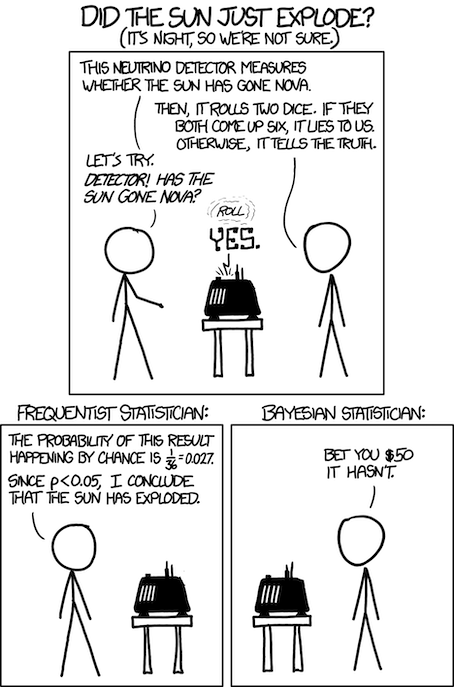
\includegraphics{images/frequentists_vs_bayesians.png}
\end{center}

\setlength{\abovedisplayskip}{-5pt}
\setlength{\abovedisplayshortskip}{-5pt}

{
\hypersetup{linkcolor=}
\setcounter{tocdepth}{2}
\tableofcontents
}
\listoffigures
\listoftables
\hypertarget{prefazione}{%
\chapter*{Prefazione}\label{prefazione}}


\emph{Data Science per psicologi} contiene il materiale delle lezioni dell'insegnamento di \emph{Psicometria B000286} (A.A. 2021/2022) rivolto agli studenti del primo anno del Corso di Laurea in Scienze e Tecniche Psicologiche dell'Università degli Studi di Firenze. \emph{Psicometria} si propone di fornire agli studenti un'introduzione all'analisi dei dati in psicologia. Le conoscenze/competenze che verranno sviluppate in questo insegnamento sono quelle della Data science, ovvero un insieme di conoscenze/competenze che si pongono all'intersezione tra statistica (ovvero, richiedono la capacità di comprendere teoremi statistici) e informatica (ovvero, richiedono la capacità di sapere utilizzare un software).

\hypertarget{la-psicologia-e-la-data-science}{%
\section*{La psicologia e la Data science}\label{la-psicologia-e-la-data-science}}


Sembra sensato spendere due parole su un tema che è importante per gli studenti: quello indicato dal titolo di questo Capitolo. È ovvio che agli studenti di psicologia la statistica non piace. Se piacesse, forse studierebbero Data science e non psicologia; ma non lo fanno. Di conseguenza, gli studenti di psicologia si chiedono: ``perché dobbiamo perdere tanto tempo a studiare queste cose quando in realtà quello che ci interessa è tutt'altro?'' Questa è una bella domanda.

C'è una ragione molto semplice che dovrebbe farci capire perché la Data science è così importante per la psicologia. Infatti, a ben pensarci, la psicologia è una disciplina intrinsecamente statistica, se per statistica intendiamo quella disciplina che studia la variazione delle caratteristiche degli individui nella popolazione. La psicologia studia \emph{gli individui} ed è proprio la variabilità inter- e intra-individuale ciò che vogliamo descrivere e, in certi casi, predire. In questo senso, la psicologia è molto diversa dall'ingegneria, per esempio. Le proprietà di un determinato ponte sotto certe condizioni, ad esempio, sono molto simili a quelle di un altro ponte, sotto le medesime condizioni. Quindi, per un ingegnere la statistica è poco importante: le proprietà dei materiali sono unicamente dipendenti dalla loro composizione e restano costanti. Ma lo stesso non può dirsi degli individui: ogni individuo è unico e cambia nel tempo. E le variazioni tra gli individui, e di un individuo nel tempo, sono l'oggetto di studio proprio della psicologia: è dunque chiaro che i problemi che la psicologia si pone sono molto diversi da quelli affrontati, per esempio, dagli ingegneri. Questa è la ragione per cui abbiamo tanto bisogno della Data science in psicologia: perché la Data science ci consente di descrivere la variazione e il cambiamento. E queste sono appunto le caratteristiche di base dei fenomeni psicologici.

Sono sicuro che, leggendo queste righe, a molti studenti sarà venuta in mente la seguente domanda: perché non chiediamo a qualche esperto di fare il ``lavoro sporco'' (ovvero le analisi statistiche) per noi, mentre noi (gli psicologi) ci occupiamo solo di ciò che ci interessa, ovvero dei problemi psicologici slegati dai dettagli ``tecnici'' della Data science? La risposta a questa domanda è che non è possibile progettare uno studio psicologico sensato senza avere almeno una comprensione rudimentale della Data science. Le tematiche della Data science non possono essere ignorate né dai ricercatori in psicologia né da coloro che svolgono la professione di psicologo al di fuori dell'Università. Infatti, anche i professionisti al di fuori dall'università non possono fare a meno di leggere la letteratura psicologica più recente: il continuo aggiornamento delle conoscenze è infatti richiesto dalla deontologia della professione. Ma per potere fare questo è necessario conoscere un bel po' di Data science! Basta aprire a caso una rivista specialistica di psicologia per rendersi conto di quanto ciò sia vero: gli articoli che riportano i risultati delle ricerche psicologiche sono zeppi di analisi statistiche e di modelli formali. E la comprensione della letteratura psicologica rappresenta un requisito minimo nel bagaglio professionale dello psicologo.

Le considerazioni precedenti cercano di chiarire il seguente punto: la Data science non è qualcosa da studiare a malincuore, in un singolo insegnamento universitario, per poi poterla tranquillamente dimenticare. Nel bene e nel male, gli psicologi usano gli strumenti della Data science in tantissimi ambiti della loro attività professionale: in particolare quando costruiscono, somministrano e interpretano i test psicometrici. È dunque chiaro che possedere delle solide basi di Data science è un tassello imprescindibile del bagaglio professionale dello psicologo. In questo insegnamento verrano trattati i temi base della Data science e verrà adottato un punto di vista bayesiano, che corrisponde all'approccio più recente e sempre più diffuso in psicologia.

\hypertarget{come-studiare}{%
\section*{Come studiare}\label{come-studiare}}


Il giusto metodo di studio per prepararsi all'esame di Psicometria è quello di seguire attivamente le lezioni, assimilare i concetti via via che essi vengono presentati e verificare in autonomia le procedure presentate a lezione. Incoraggio gli studenti a farmi domande per chiarire ciò che non è stato capito appieno. Incoraggio gli studenti a utilizzare i forum attivi su Moodle e, soprattutto, a svolgere gli esercizi proposti su Moodle. I problemi forniti su Moodle rappresentano il livello di difficoltà richiesto per superare l'esame e consentono allo studente di comprendere se le competenze sviluppate fino a quel punto sono sufficienti rispetto alle richieste dell'esame.

La prima fase dello studio, che è sicuramente individuale, è quella in cui è necessario acquisire le conoscenze teoriche relative ai problemi che saranno presentati all'esame. La seconda fase di studio, che può essere facilitata da scambi con altri e da incontri di gruppo, porta ad acquisire la capacità di applicare le conoscenze: è necessario capire come usare un software (\(\textsf{R}\)) per applicare i concetti statistici alla specifica situazione del problema che si vuole risolvere. Le due fasi non sono però separate: il saper fare molto spesso ci aiuta a capire meglio.

\hypertarget{sviluppare-un-metodo-di-studio-efficace}{%
\section*{Sviluppare un metodo di studio efficace}\label{sviluppare-un-metodo-di-studio-efficace}}


Avendo insegnato molte volte in passato un corso introduttivo di analisi dei dati ho notato nel corso degli anni che gli studenti con l'atteggiamento mentale che descriverò qui sotto generalmente ottengono ottimi risultati. Alcuni studenti sviluppano naturalmente questo approccio allo studio, ma altri hanno bisogno di fare uno sforzo per maturarlo. Fornisco qui sotto una breve descrizione del ``metodo di studio'' che, nella mia esperienza, è il più efficace per affrontare le richieste di questo insegnamento.

\begin{itemize}
\tightlist
\item
  Dedicate un tempo sufficiente al materiale di base, apparentemente facile; assicuratevi di averlo capito bene. Cercate le lacune nella vostra comprensione. Leggere presentazioni diverse dello stesso materiale (in libri o articoli diversi) può fornire nuove intuizioni.
\item
  Gli errori che facciamo sono i nostri migliori maestri. Istintivamente cerchiamo di dimenticare subito i nostri errori. Ma il miglior modo di imparare è apprendere dagli errori che commettiamo. In questo senso, una soluzione corretta è meno utile di una soluzione sbagliata. Quando commettiamo un errore questo ci fornisce un'informazione importante: ci fa capire qual è il materiale di studio sul quale dobbiamo ritornare e che dobbiamo capire meglio.
\item
  C'è ovviamente un aspetto ``psicologico'' nello studio. Quando un esercizio o problema ci sembra incomprensibile, la cosa migliore da fare è dire: ``mi arrendo'', ``non ho idea di cosa fare!''. Questo ci rilassa: ci siamo già arresi, quindi non abbiamo niente da perdere, non dobbiamo più preoccuparci. Ma non dobbiamo fermarci qui. Le cose ``migliori'' che faccio (se ci sono) le faccio quando non ho voglia di lavorare. Alle volte, quando c'è qualcosa che non so fare e non ho idea di come affontare, mi dico: ``oggi non ho proprio voglia di fare fatica'', non ho voglia di mettermi nello stato mentale per cui ``in 10 minuti devo risolvere il problema perché dopo devo fare altre cose''. Però ho voglia di \emph{divertirmi} con quel problema e allora mi dedico a qualche aspetto ``marginale'' del problema, che so come affrontare, oppure considero l'aspetto più difficile del problema, quello che non so come risolvere, ma invece di cercare di risolverlo, guardo come altre persone hanno affrontato problemi simili, opppure lo stesso problema in un altro contesto. Non mi pongo l'obiettivo ``risolvi il problema in 10 minuti'', ma invece quello di farmi un'idea ``generale'' del problema, o quello di capire un caso più specifico e più semplice del problema. Senza nessuna pressione. Infatti, in quel momento ho deciso di non lavorare (ovvero, di non fare fatica). Va benissimo se ``parto per la tangente'', ovvero se mi metto a leggere del materiale che sembra avere poco a che fare con il problema centrale (le nostre intuizioni e la nostra curiosità solitamente ci indirizzano sulla strada giusta). Quando faccio così, molto spesso trovo la soluzione del problema che mi ero posto e, paradossalmente, la trovo in un tempo minore di quello che, in precedenza, avevo dedicato a ``lavorare'' al problema. Allora perché non faccio sempre così? C'è ovviamente l'aspetto dei ``10 minuti'' che non è sempre facile da dimenticare. Sotto pressione, possiamo solo agire in maniera automatica, ovvero possiamo solo applicare qualcosa che già sappiamo fare. Ma se dobbiamo imparare qualcosa di nuovo, la pressione è un impedimento.
\item
  È utile farsi da soli delle domande sugli argomenti trattati, senza limitarsi a cercare di risolvere gli esercizi che vengono assegnati. Quando studio qualcosa mi viene in mente: ``se questo è vero, allora deve succedere quest'altra cosa''. Allora verifico se questo è vero, di solito con una simulazione. Se i risultati della simulazione sono quelli che mi aspetto, allora vuol dire che ho capito. Se i risultati sono diversi da quelli che mi aspettavo, allora mi rendo conto di non avere capito e ritorno indietro a studiare con più attenzione la teoria che pensavo di avere capito -- e ovviamente mi rendo conto che c'era un aspetto che avevo frainteso. Questo tipo di verifica è qualcosa che dobbiamo fare da soli, in prima persona: nessun altro può fare questo al posto nostro.
\item
  Non aspettatevi di capire tutto la prima volta che incontrate un argomento nuovo.\footnote{Ricordatevi inoltre che gli individui tendono a sottostimare la propria capacità di apprendere \citep{horn2021underestimating}.} È utile farsi una nota mentalmente delle lacune nella vostra comprensione e tornare su di esse in seguito per carcare di colmarle. L'atteggiamento naturale, quando non capiamo i dettagli di qualcosa, è quello di pensare: ``non importa, ho capito in maniera approssimativa questo punto, non devo preoccuparmi del resto''. Ma in realtà non è vero: se la nostra comprensione è superficiale, quando il problema verrà presentato in una nuova forma, non riusciremo a risolverlo. Per cui i dubbi che ci vengono quando studiamo qualcosa sono il nostro alleato più prezioso: ci dicono esattamente quali sono gli aspetti che dobbiamo approfondire per potere migliorare la nostra preparazione.
\item
  È utile sviluppare una visione d'insieme degli argomenti trattati, capire l'obiettivo generale che si vuole raggiungere e avere chiaro il contributo che i vari pezzi di informazione forniscono al raggiungimento di tale obiettivo. Questa organizzazione mentale del materiale di studio facilita la comprensione. È estremamente utile creare degli schemi di ciò che si sta studiando. Non aspettate che sia io a fornirvi un riepilogo di ciò che dovete imparare: sviluppate da soli tali schemi e tali riassunti.
\item
  Tutti noi dobbiamo imparare l'arte di trovare le informazioni, non solo nel caso di questo insegnamento. Quando vi trovate di fronte a qualcosa che non capite, o ottenete un oscuro messaggio di errore da un software, ricordatevi: ``Google is your friend''!
\end{itemize}

\begin{flushright}
Corrado Caudek\\
Marzo 2022 \end{flushright}

\mainmatter

\hypertarget{part-il-calcolo-delle-probabilituxe0}{%
\part{Il calcolo delle probabilità}\label{part-il-calcolo-delle-probabilituxe0}}

\hypertarget{intro-prob-1}{%
\chapter{La logica dell'incerto}\label{intro-prob-1}}

In questa parte della dispensa verrà introdotta la teoria delle probabilità. Prima di entrare nei dettagli, cerchiamo di capire perché la probabilità sia cruciale per la ricerca scientifica.

La teoria delle probabilità è cruciale per la scienza perché la ricerca procede mediante l'inferenza induttiva. Non siamo mai completamente sicuri della verità di una proposizione (ipotesi, teoria): al valore di verità di una proposizione possiamo solo assegnare un giudizio probabilistico. L'approccio bayesiano è una scuola di pensiero che usa la probabilità per quantificare il grado di fiducia che può essere attribuito ad una proposizione. L'inferenza statistica bayesiana è un tipo di inferenza induttiva che ha lo scopo di quantificare la fiducia che si ha nell'ipotesi \(H\) dopo il verificarsi del dato d'evidenza \(E\). Per quantificare un tale grado di fiducia l'inferenza statistica bayesiana utilizza la teoria delle probabilità. Una comprensione dell'inferenza statistica bayesiana richiede dunque, preliminarmente, la conoscenze della teoria delle probabilità.

\hypertarget{che-cosuxe8-la-probabilituxe0}{%
\section{Che cos'è la probabilità?}\label{che-cosuxe8-la-probabilituxe0}}

La definizione della probabilità è un problema estremamente dibattuto ed aperto. Sono state fornite due possibili soluzioni al problema di definire il concetto di probabilità.

\begin{enumerate}
\def\labelenumi{(\alph{enumi})}
\item
  La natura della probabilità è ``ontologica'' (ovvero, basata sulla metafisica): la probabilità è una proprietà della della realtà, del mondo, di come sono le cose, indipendentemente dalla nostra esperienza. È una visione che qualcuno chiama ``oggettiva''.
\item
  La natura della probabilità è ``epistemica'' (ovvero, basata sulla conoscenza): la probabilità si riferisce alla conoscenza che abbiamo del mondo, non al mondo in sé. Di conseguenza è detta, in contrapposizione alla precedente definizione, ``soggettiva''.
\end{enumerate}

In termini epistemici, la probabilità fornisce una misura della nostra incertezza sul verificarsi di un fenomeno, alla luce delle informazioni disponibili. Potremmo dire che c'è una ``scala'' naturale che ha per estremi il vero (1: evento certo) da una parte ed il falso (0: evento impossibile) dall'altra. La probabilità è la quantificazione di questa scala: descrive lo stato della nostra incertezza rispetto al contenuto di verità di una proposizione.

Nell'interpretazione frequentista, la probabilità \(P(E)\) rappresenta la frequenza relativa a lungo termine di un grande numero di ripetizioni di un esperimento casuale sotto le medesime condizioni. Viene stressata qui l'idea che ciò di cui parliamo è qualcosa che emerge nel momento in cui è possibile ripetere l'esperimento casuale tante volte sotto le medesime condizioni -- sono invece esclusi gli eventi unici e irripetibili.

L'interpretazione bayesiana della probabilità fa invece ricorso ad una concezione più ampia, non legata al solo evento in sé ma che include anche il soggetto assegnante la funzione di probabilità. In pratica l'assegnazione di probabilità bayesiana viene effettuata dal decisore, in base alle proprie conoscenze a priori integrate con tutto il generico bagaglio culturale personale. In questo modo, la probabilità non sarà obbligatoriamente la stessa per tutti i soggetti, ma variarierà a seconda delle informazioni a disposizione, dell'esperienza personale e soprattutto del punto di vista proprio di ogni decisore ed è dunque assimilabile al ``grado di fiducia'' -- in inglese \emph{degree of belief} -- di un dato soggetto, in un dato istante e con un dato insieme d'informazioni, circa l'accadere dell'evento \(E\). ``{[}N{]}essuna scienza ci permetterà di dire: il tale fatto accadrà, andrà così e così, perché ciò è conseguenza di tale legge, e tale legge è una verità assoluta, ma tanto meno ci condurrà a concludere scetticamente: la verità assoluta non esiste, e quindi tale fatto può accadere e può non accadere, può andare così e può andare in tutt'altro modo, nulla io ne so. Quel che si potrà dire è questo: io prevedo che il tale fatto avverrà, e avverrà nel tal modo, perché l'esperienza del passato e l'elaborazione scientifica cui il pensiero dell'uomo l'ha sottoposta mi fanno sembrare ragionevole questa previsione'' \citep{definetti1931prob}.

L'impostazione bayesiana, sviluppata da Ramsey e de Finetti, riconduce l'assegnazione di probabilità allo scommettere sul verificarsi di un evento: la probabilità di un evento \(E\) è la quota \(p(E)\) che un individuo reputa di dover pagare ad un banco per ricevere ``1'' ovvero ``0'' verificandosi o non verificandosi \(E\).

Secondo De Finetti, le valutazioni di probabilità degli eventi devono rispondere ai principi di equità e coerenza. Una scommessa risponde al principio di \emph{equità} se il ruolo di banco e giocatore sono scambiabili in ogni momento del gioco e sempre alle stesse condizioni. Una scommessa risponde al principio di \emph{coerenza} se non vi sono combinazioni di scommesse che consentano (sia al banco che al giocatore) di realizzare perdite o vincite certe.

L'approccio definettiano dell'impostazione della scommessa si basa dunque sulle assunzioni di razionalità e coerenza del decisore, al quale è fatto esplicito divieto di effettuare scommesse a perdita o guadagno certo. Il decisore, proponendo la scommessa, deve essere disposto a scambiare il posto dello scommettitore con quello del banco.

Il metodo della scommessa, oltre che una definizione, fornisce un mezzo operativo di assegnazione della probabilità. Sulla base di questa definizione operativa, che si può ritenere ragionevolmente soddisfatta dal comportamento di un qualunque individuo che agisca in modo razionale in condizioni di incertezza, possono essere agevolmente dimostrate tutte le proprietà classiche della probabilità: essa non può assumere valori negativi, né può essere superiore all'unità; se \(E\) è un evento certo, la sua probabilità è 1; se invece \(E\) è un evento impossibile, la sua probabilità è 0.

I problemi posti dall'approccio definettiano riguardano l'arbitrarietà dell'assegnazione soggettività di probabilità la quale sembra negare la validità dell'intero costrutto teorico. In risposta a tale critica, i bayesiani sostengono che gli approcci oggettivisti alla probabilità nascondono scelte arbitrarie preliminari e sono basate su assunzioni implausibili. È molto più onesto esplicitare subito tutte le scelte arbitrarie effettuate nel corso dell'analisi in modo da controllarne coerenza e razionalità.

\hypertarget{variabili-casuali-e-probabilituxe0-di-un-evento}{%
\section{Variabili casuali e probabilità di un evento}\label{variabili-casuali-e-probabilituxe0-di-un-evento}}

Esaminiamo qui di seguito alcuni concetti di base della teoria delle probabilità.

\hypertarget{eventi-e-probabilituxe0}{%
\subsection{Eventi e probabilità}\label{eventi-e-probabilituxe0}}

Nella teoria delle probabilità il risultato ``testa'' nel lancio di una moneta è chiamato \emph{evento}.\footnote{Per un ripasso delle nozioni di base della teoria degli insiemi, si veda l'Appendice \ref{insiemistica}.} Ad esempio, \(Y\) = 1 denota l'evento in cui il lancio di una moneta produce come risultato testa. Il funzionale \(P(·)\) definisce la probabilità di un evento. Ad esempio, per il lancio di una moneta equilibrata, la probabilità dell'evento ``il risultato del lancio della moneta è testa'' è scritta come \(P(Y = 1) = 0.5.\)

Se la moneta è equilibrata dobbiamo anche avere \(P(Y = 0) = 0.5\). I due eventi \emph{Y} = 1 e \(Y\) = 0 sono \emph{mutuamente esclusivi} nel senso che non possono entrambi verificarsi contemporaneamente: \(P(Y = 1\; e \; Y = 0) = 0.\) Gli eventi \(Y\) = 1 e \(Y\) = 0 di dicono \emph{esaustivi}, nel senso che almeno uno di essi deve verificarsi e nessun altro tipo di evento è possibile. Nella notazione probabilistica, \(P(Y = 1\; o \; Y = 0) = 1.\)

Il connettivo logico ``o'' specifica eventi \emph{disgiunti}, ovvero eventi che non possono verificarsi contemporaneamente (eventi \emph{incompatibili}) e per i quali, perciò, la probabilità della loro congiunzione è \(P(A \; e \; B) = 0\). Il connettivo logico ``e'', invece, specifica eventi \emph{congiunti}, ovvero eventi che possono verificarsi contemporaneamente (eventi \emph{compatibili}) e per i quali, perciò, la probabilità della loro congiunzione è \(P(A \; e \; B) > 0\).

\hypertarget{spazio-campione-e-risultati-possibili}{%
\subsection{Spazio campione e risultati possibili}\label{spazio-campione-e-risultati-possibili}}

Anche se il lancio di una moneta produce sempre uno specifico risultato nel mondo reale, possiamo anche immaginare i possibili risultati alternativi che si sarebbero potuti osservare. Quindi, anche se in uno specifico lancio la moneta dà testa (\(Y\) = 1), possiamo immaginare la possibilità che il lancio possa avere prodotto croce (\(Y\) = 0). Tale ragionamento controfattuale è la chiave per comprendere la teoria delle probabilità e l'inferenza statistica.

I risultati possibili che si possono osservare come conseguenza del lancio di una moneta determinano i valori possibili che la variabile casuale può assumere. L'insieme \(\Omega\) di tutti i risultati possibili è chiamato \emph{spazio campione} (\emph{sample space}). Lo spazio campione può essere concettualizzato come un'urna contenente una pallina per ogni possibile risultato del lancio della moneta. Su ogni pallina è scritto il valore della variabile casuale. Uno specifico lancio di una moneta -- ovvero, l'osservazione di uno specifico valore di una variabile casuale -- è chiamato \emph{esperimento casuale}.

Il lancio di un dado ci fornisce l'esempio di un altro esperimento casuale. Supponiamo di essere interessati all'evento ``il lancio del dado produce un numero dispari''. Un \emph{evento} seleziona un sottoinsieme dello spazio campione: in questo caso, l'insieme dei risultati \(\{1, 3, 5\}\). Se esce 3, per esempio, diciamo che si è verificato l'evento ``dispari'' (ma l'evento ``dispari'' si sarebbe anche verificato anche se fosse uscito 1 o 5).

\hypertarget{variabili-casuali}{%
\section{Variabili casuali}\label{variabili-casuali}}

Sia \(Y\) il risultato del lancio di moneta equilibrata, non di un generico lancio di una moneta, ma un'istanza specifica del lancio di una specifica moneta in un dato momento. Definita in questo modo, \(Y\) è una \emph{variabile casuale}, ovvero una variabile i cui valori non possono essere previsti con esattezza. Se la moneta è equilibrata, c'è una probabilità del 50\% che il lancio della moneta dia come risultato ``testa'' e una probabilità del 50\% che dia come risultato ``croce''. Per facilitare la trattazione, le variabili casuali assumono solo valori numerici. Per lo specifico lancio della moneta in questione, diciamo, ad esempio, che la variabile casuale \(Y\) assume il valore 1 se esce testa e il valore 0 se esce croce.

Una variabile casuale può essere \emph{discreta} o \emph{continua}. Una variabile casuale discreta può assumere un numero finito di valori \(x_1, \dots ,x_n\), in corrispondenza degli eventi \(E_i, \dots, E_n\) che si verificano con le rispettive probabilità \(p_1, \dots, p_n\). Un esempio è il punteggio totale di un test psicometrico costituito da item su scala Likert. Invece un esempio di una variabile casuale continua è la distanza tra due punti, che può assumere infiniti valori all'interno di un certo intervallo. L'insieme \(S\) dei valori che la variabile casuale può assumere è detto \emph{spazio dei valori} o \emph{spazio degli stati}. La caratteristica fondamentale di una variabile casuale è data dall'insieme delle probabilità dei suoi valori, detta \emph{distribuzione di probabilità}. Nel seguito useremo la notazione \(P(\cdot)\) per fare riferimento alle distribuzioni di probabilità delle variabili casuali discrete e \(p(\cdot)\) per fare riferimento alla densità di probabilità delle variabili casuali continue. In questo contesto, l'insieme dei valori che la variabile casuale può assumere è detto \emph{supporto} della sua distribuzione di probabilità. Il supporto di una variabile casuale può essere finito (come nel caso di una variabile casuale uniforme di supporto \([a, b]\)) o infinito (nel caso di una variabile causale gaussiana il cui supporto coincide con la retta reale).

\hypertarget{usare-la-simulazione-per-stimare-le-probabilituxe0}{%
\section{Usare la simulazione per stimare le probabilità}\label{usare-la-simulazione-per-stimare-le-probabilituxe0}}

I metodi basati sulla simulazione consentono di stimare le probabilità degli eventi in un modo diretto, se siamo in grado di generare molteplici e casuali realizzazioni delle variabili casuali coinvolte nelle definizioni degli eventi. Per simulare il lancio di una moneta equilibrata in \(\R\) iniziamo a definire un vettore che contiene i possibili risultati del lancio della moneta (ovvero i possibili valori della variabile casuale \(Y\)):

\begin{Shaded}
\begin{Highlighting}[]
\NormalTok{coin }\OtherTok{\textless{}{-}} \FunctionTok{c}\NormalTok{(}\DecValTok{0}\NormalTok{, }\DecValTok{1}\NormalTok{)}
\end{Highlighting}
\end{Shaded}

\noindent L'estrazione casuale di uno di questi due possibili valori (ovvero, la simulazione di uno specifico lancio di una moneta) si realizza con la funzione \texttt{sample()}:

\begin{Shaded}
\begin{Highlighting}[]
\FunctionTok{sample}\NormalTok{(coin, }\AttributeTok{size =} \DecValTok{1}\NormalTok{)}
\CommentTok{\#\textgreater{} [1] 0}
\end{Highlighting}
\end{Shaded}

\noindent In maniera equivalente, la stessa operazione si può realizzare mediante l'istruzione

\begin{Shaded}
\begin{Highlighting}[]
\FunctionTok{rbinom}\NormalTok{(}\DecValTok{1}\NormalTok{, }\DecValTok{1}\NormalTok{, }\FloatTok{0.5}\NormalTok{)}
\CommentTok{\#\textgreater{} [1] 1}
\end{Highlighting}
\end{Shaded}

Supponiamo di ripetere questo esperimento casuale 100 volte e di registrare i risultati così ottenuti. La stima della probabilità dell'evento \(P(Y = 1)\) è data dalla frequenza relativa del numero di volte in cui abbiamo osservato l'evento di interesse (\(Y = 1\)):

\begin{Shaded}
\begin{Highlighting}[]
\NormalTok{M }\OtherTok{\textless{}{-}} \DecValTok{100}
\NormalTok{y }\OtherTok{\textless{}{-}} \FunctionTok{rep}\NormalTok{(}\ConstantTok{NA}\NormalTok{, M)}
\ControlFlowTok{for}\NormalTok{ (m }\ControlFlowTok{in} \DecValTok{1}\SpecialCharTok{:}\NormalTok{M) \{}
\NormalTok{  y[m] }\OtherTok{\textless{}{-}} \FunctionTok{rbinom}\NormalTok{(}\DecValTok{1}\NormalTok{, }\DecValTok{1}\NormalTok{, }\FloatTok{0.5}\NormalTok{)}
\NormalTok{\}}
\NormalTok{estimate }\OtherTok{\textless{}{-}} \FunctionTok{sum}\NormalTok{(y) }\SpecialCharTok{/}\NormalTok{ M}

\FunctionTok{cat}\NormalTok{(}\StringTok{"estimated Pr[Y = 1] ="}\NormalTok{, estimate)}
\CommentTok{\#\textgreater{} estimated Pr[Y = 1] = 0.53}
\end{Highlighting}
\end{Shaded}

Ripetiamo questa procedura 10 volte.

\begin{Shaded}
\begin{Highlighting}[]
\NormalTok{flip\_coin }\OtherTok{\textless{}{-}} \ControlFlowTok{function}\NormalTok{(M) \{}
\NormalTok{  y }\OtherTok{\textless{}{-}} \FunctionTok{rep}\NormalTok{(}\ConstantTok{NA}\NormalTok{, M)}
  \ControlFlowTok{for}\NormalTok{ (m }\ControlFlowTok{in} \DecValTok{1}\SpecialCharTok{:}\NormalTok{M) \{}
\NormalTok{    y[m] }\OtherTok{\textless{}{-}} \FunctionTok{rbinom}\NormalTok{(}\DecValTok{1}\NormalTok{, }\DecValTok{1}\NormalTok{, }\FloatTok{0.5}\NormalTok{)}
\NormalTok{  \}}
\NormalTok{  estimate }\OtherTok{\textless{}{-}} \FunctionTok{sum}\NormalTok{(y) }\SpecialCharTok{/}\NormalTok{ M}
  \FunctionTok{cat}\NormalTok{(}\StringTok{"estimated Pr[Y = 1] ="}\NormalTok{, estimate, }\StringTok{"}\SpecialCharTok{\textbackslash{}n}\StringTok{"}\NormalTok{)}
\NormalTok{\}}
\end{Highlighting}
\end{Shaded}

\begin{Shaded}
\begin{Highlighting}[]
\ControlFlowTok{for}\NormalTok{ (i }\ControlFlowTok{in} \DecValTok{1}\SpecialCharTok{:}\DecValTok{10}\NormalTok{) \{}
  \FunctionTok{flip\_coin}\NormalTok{(}\DecValTok{100}\NormalTok{)}
\NormalTok{\}}
\CommentTok{\#\textgreater{} estimated Pr[Y = 1] = 0.44 }
\CommentTok{\#\textgreater{} estimated Pr[Y = 1] = 0.52 }
\CommentTok{\#\textgreater{} estimated Pr[Y = 1] = 0.46 }
\CommentTok{\#\textgreater{} estimated Pr[Y = 1] = 0.57 }
\CommentTok{\#\textgreater{} estimated Pr[Y = 1] = 0.47 }
\CommentTok{\#\textgreater{} estimated Pr[Y = 1] = 0.46 }
\CommentTok{\#\textgreater{} estimated Pr[Y = 1] = 0.48 }
\CommentTok{\#\textgreater{} estimated Pr[Y = 1] = 0.49 }
\CommentTok{\#\textgreater{} estimated Pr[Y = 1] = 0.47 }
\CommentTok{\#\textgreater{} estimated Pr[Y = 1] = 0.62}
\end{Highlighting}
\end{Shaded}

Dato che la moneta è equilibrata, la stima delle probabilità dell'evento \(Pr[Y = 1]\) è simile a al valore che ci aspettiamo (\(P(Y = 1)\) = 0.5), ma il risultato ottenuto nelle varie simulazioni non è sempre esatto. Proviamo ad aumentare il numero di lanci in ciascuna simulazione:

\begin{Shaded}
\begin{Highlighting}[]
\ControlFlowTok{for}\NormalTok{ (i }\ControlFlowTok{in} \DecValTok{1}\SpecialCharTok{:}\DecValTok{10}\NormalTok{) \{}
  \FunctionTok{flip\_coin}\NormalTok{(}\DecValTok{1000}\NormalTok{)}
\NormalTok{\}}
\CommentTok{\#\textgreater{} estimated Pr[Y = 1] = 0.497 }
\CommentTok{\#\textgreater{} estimated Pr[Y = 1] = 0.529 }
\CommentTok{\#\textgreater{} estimated Pr[Y = 1] = 0.493 }
\CommentTok{\#\textgreater{} estimated Pr[Y = 1] = 0.511 }
\CommentTok{\#\textgreater{} estimated Pr[Y = 1] = 0.506 }
\CommentTok{\#\textgreater{} estimated Pr[Y = 1] = 0.52 }
\CommentTok{\#\textgreater{} estimated Pr[Y = 1] = 0.49 }
\CommentTok{\#\textgreater{} estimated Pr[Y = 1] = 0.495 }
\CommentTok{\#\textgreater{} estimated Pr[Y = 1] = 0.489 }
\CommentTok{\#\textgreater{} estimated Pr[Y = 1] = 0.496}
\end{Highlighting}
\end{Shaded}

In questo secondo caso, gli errori tendono ad essere più piccoli della simulazione precedente. Cosa succede se in ciascuna simulazione esaminiamo i risultati di 10,000 lanci della moneta?

\begin{Shaded}
\begin{Highlighting}[]
\ControlFlowTok{for}\NormalTok{ (i }\ControlFlowTok{in} \DecValTok{1}\SpecialCharTok{:}\DecValTok{10}\NormalTok{) \{}
  \FunctionTok{flip\_coin}\NormalTok{(}\FloatTok{1e4}\NormalTok{)}
\NormalTok{\}}
\CommentTok{\#\textgreater{} estimated Pr[Y = 1] = 0.4885 }
\CommentTok{\#\textgreater{} estimated Pr[Y = 1] = 0.4957 }
\CommentTok{\#\textgreater{} estimated Pr[Y = 1] = 0.4902 }
\CommentTok{\#\textgreater{} estimated Pr[Y = 1] = 0.5032 }
\CommentTok{\#\textgreater{} estimated Pr[Y = 1] = 0.5048 }
\CommentTok{\#\textgreater{} estimated Pr[Y = 1] = 0.4931 }
\CommentTok{\#\textgreater{} estimated Pr[Y = 1] = 0.4965 }
\CommentTok{\#\textgreater{} estimated Pr[Y = 1] = 0.499 }
\CommentTok{\#\textgreater{} estimated Pr[Y = 1] = 0.4979 }
\CommentTok{\#\textgreater{} estimated Pr[Y = 1] = 0.4973}
\end{Highlighting}
\end{Shaded}

Ora le stime ottenute sono molto vicine alla vera probabilità che vogliamo stimare (cioè 0.5, perché la moneta è equilibrata). I risultati delle simulazioni precedenti pongono dunque il problema di determinare quale sia il numero di lanci di cui abbiamo bisogno per assicurarci che le stime siano accurate (ovvero, vicine al valore corretto della probabilità)

\hypertarget{la-legge-dei-grandi-numeri}{%
\section{La legge dei grandi numeri}\label{la-legge-dei-grandi-numeri}}

La visualizzazione mediante grafici contribuisce alla comprensione dei concetti della statistica e della teoria delle probabilità. Un modo per descrivere qjello che accade all'aumentare del numero \(M\) di ripetizioni del lancio della moneta consiste nel registrare la stima della probabilità dell'evento \(P(Y = 1)\) in funzione del numero di ripetizioni dell'esperimento casuale per ogni \(m \in 1:M\). Possiamo ottenere un grafico dell'andamento della stima di \(P(Y = 1)\) in funzione di \(m\) come:

\begin{Shaded}
\begin{Highlighting}[]
\NormalTok{nrep }\OtherTok{\textless{}{-}} \FloatTok{1e4}
\NormalTok{estimate }\OtherTok{\textless{}{-}} \FunctionTok{rep}\NormalTok{(}\ConstantTok{NA}\NormalTok{, nrep)}
\NormalTok{flip\_coin }\OtherTok{\textless{}{-}} \ControlFlowTok{function}\NormalTok{(m) \{}
\NormalTok{  y }\OtherTok{\textless{}{-}} \FunctionTok{rbinom}\NormalTok{(m, }\DecValTok{1}\NormalTok{, }\FloatTok{0.5}\NormalTok{)}
\NormalTok{  phat }\OtherTok{\textless{}{-}} \FunctionTok{sum}\NormalTok{(y) }\SpecialCharTok{/}\NormalTok{ m}
\NormalTok{  phat}
\NormalTok{\}}
\ControlFlowTok{for}\NormalTok{ (i }\ControlFlowTok{in} \DecValTok{1}\SpecialCharTok{:}\NormalTok{nrep) \{}
\NormalTok{  estimate[i] }\OtherTok{\textless{}{-}} \FunctionTok{flip\_coin}\NormalTok{(i)}
\NormalTok{\}}
\NormalTok{d }\OtherTok{\textless{}{-}} \FunctionTok{tibble}\NormalTok{(}
  \AttributeTok{n =} \DecValTok{1}\SpecialCharTok{:}\NormalTok{nrep,}
\NormalTok{  estimate}
\NormalTok{)}
\NormalTok{d }\SpecialCharTok{\%\textgreater{}\%}
  \FunctionTok{ggplot}\NormalTok{(}
    \FunctionTok{aes}\NormalTok{(}\AttributeTok{x =}\NormalTok{ n, }\AttributeTok{y =}\NormalTok{ estimate)}
\NormalTok{  ) }\SpecialCharTok{+}
  \FunctionTok{geom\_line}\NormalTok{() }\SpecialCharTok{+}
  \FunctionTok{theme}\NormalTok{(}\AttributeTok{legend.title =} \FunctionTok{element\_blank}\NormalTok{()) }\SpecialCharTok{+}
  \FunctionTok{labs}\NormalTok{(}
    \AttributeTok{x =} \StringTok{"Numero di lanci della moneta"}\NormalTok{,}
    \AttributeTok{y =} \StringTok{"Stima Pr[Y = 1]"}
\NormalTok{  )}
\end{Highlighting}
\end{Shaded}

\begin{figure}

{\centering 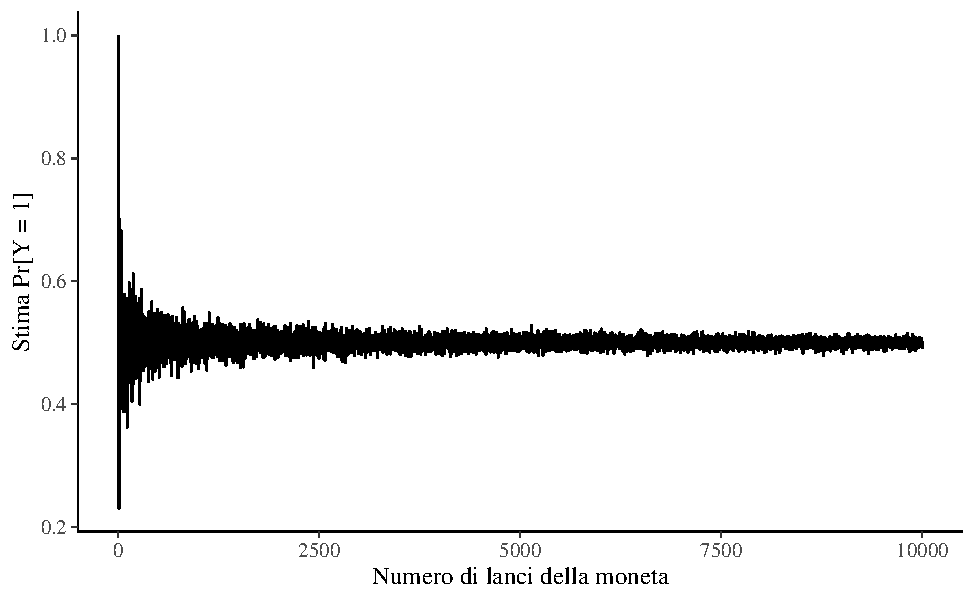
\includegraphics{ds4psy_files/figure-latex/legge-grandi-n-1-1} 

}

\caption{Stima della probabilità di successo in funzione del numero di lanci di una moneta.}\label{fig:legge-grandi-n-1}
\end{figure}

Dato che il grafico \ref{fig:legge-grandi-n-1} espresso su una scala lineare non rivela chiaramente l'andamento della simulazione, imponiamo una scala logaritmica sull'asse delle ascisse (\(x\)). Su scala logaritmica, i valori tra 1 e 10 vengono tracciati all'incirca con la stessa ampiezza che si osserva tra i valori 50 e 700, eccetera.

\begin{Shaded}
\begin{Highlighting}[]
\NormalTok{d }\SpecialCharTok{\%\textgreater{}\%}
  \FunctionTok{ggplot}\NormalTok{(}
    \FunctionTok{aes}\NormalTok{(}\AttributeTok{x =}\NormalTok{ n, }\AttributeTok{y =}\NormalTok{ estimate)}
\NormalTok{  ) }\SpecialCharTok{+}
  \FunctionTok{geom\_line}\NormalTok{() }\SpecialCharTok{+}
  \FunctionTok{scale\_x\_log10}\NormalTok{(}
    \AttributeTok{breaks =} \FunctionTok{c}\NormalTok{(}
      \DecValTok{1}\NormalTok{, }\DecValTok{3}\NormalTok{, }\DecValTok{10}\NormalTok{, }\DecValTok{50}\NormalTok{, }\DecValTok{200}\NormalTok{,}
      \DecValTok{700}\NormalTok{, }\DecValTok{2500}\NormalTok{, }\DecValTok{10000}
\NormalTok{    )}
\NormalTok{  ) }\SpecialCharTok{+}
  \FunctionTok{theme}\NormalTok{(}\AttributeTok{legend.title =} \FunctionTok{element\_blank}\NormalTok{()) }\SpecialCharTok{+}
  \FunctionTok{labs}\NormalTok{(}
    \AttributeTok{x =} \StringTok{"Numero di lanci della moneta"}\NormalTok{,}
    \AttributeTok{y =} \StringTok{"Stima Pr[Y = 1]"}
\NormalTok{  )}
\end{Highlighting}
\end{Shaded}

\begin{figure}

{\centering 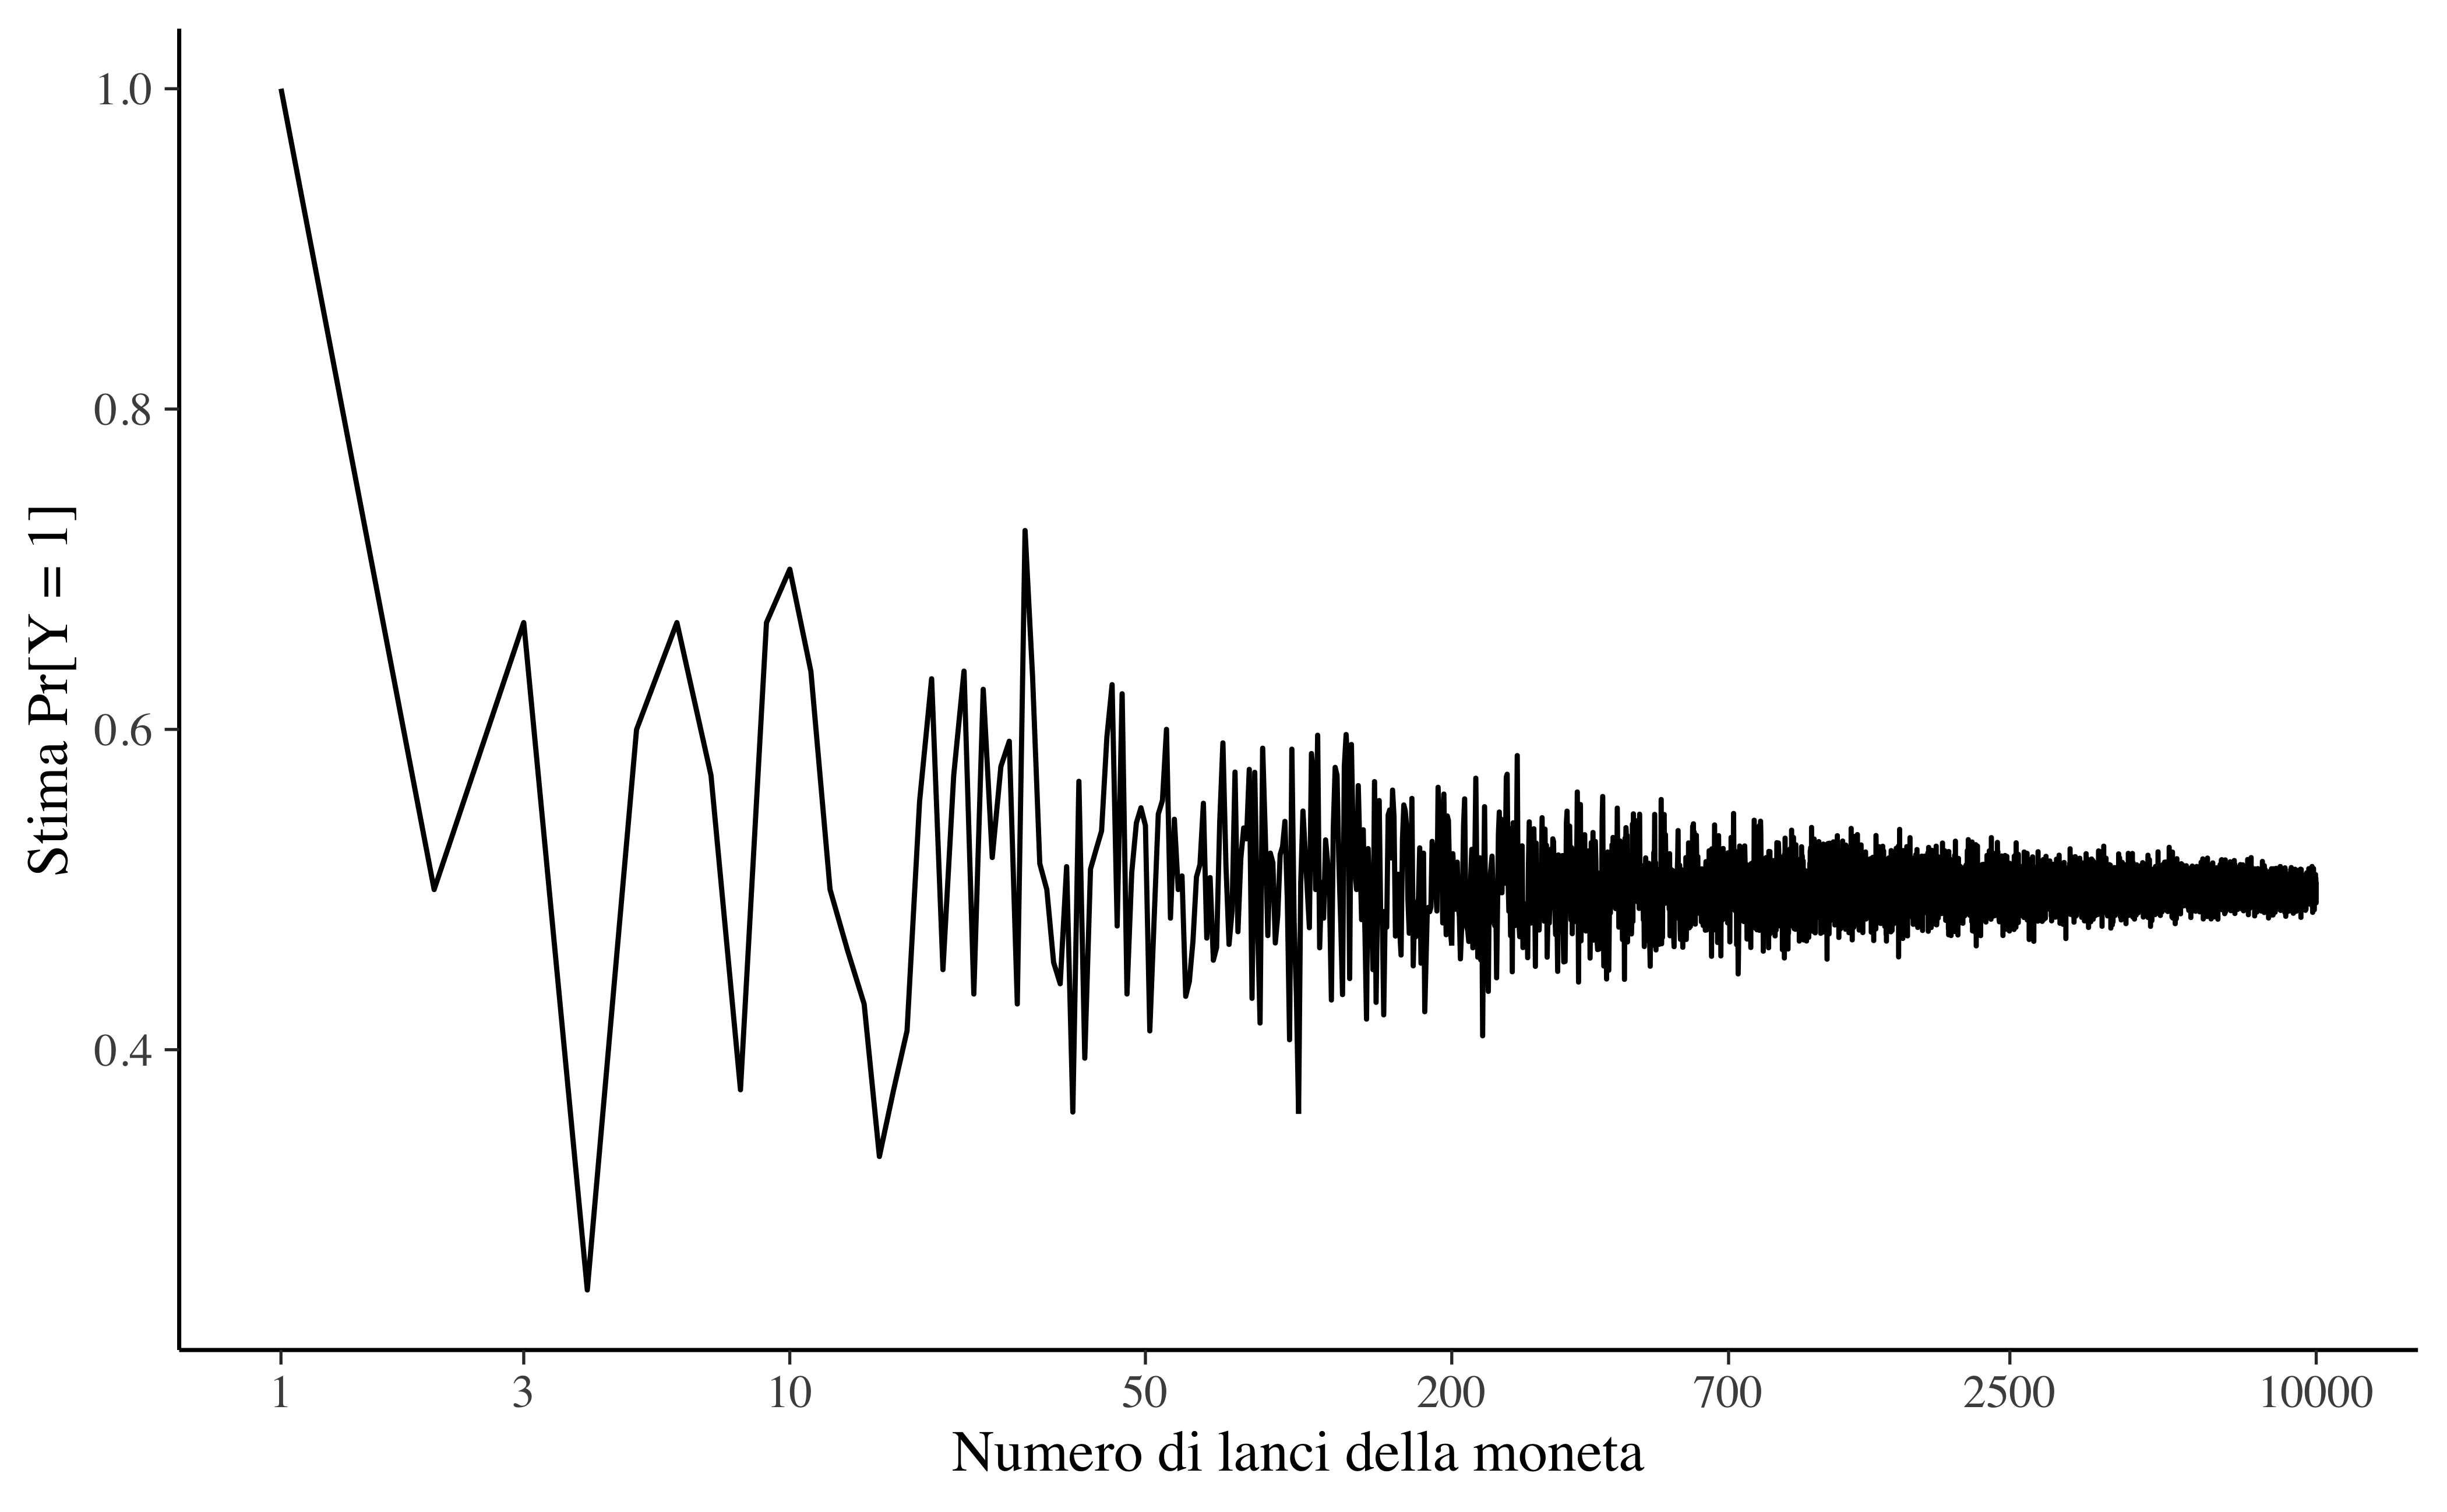
\includegraphics{ds4psy_files/figure-latex/legge-grandi-n-2-1} 

}

\caption{Stima della probabilità di successo in funzione del numero di lanci di una moneta -- scala logaritmica.}\label{fig:legge-grandi-n-2}
\end{figure}

La \emph{legge dei grandi numeri} ci dice che, all'aumentare del numero di ripetizioni dell'esperimento casuale, la media dei risultati ottenuti tende al valore atteso, man mano che vengono eseguite più prove. Nella figura \ref{fig:legge-grandi-n-2} vediamo infatti che, all'aumentare del numero \emph{M} di lanci della moneta, la stima di \(P(Y = 1)\) converge al valore 0.5.

\hypertarget{variabili-casuali-multiple}{%
\section{Variabili casuali multiple}\label{variabili-casuali-multiple}}

Le variabili casuali non esistono isolatamente. Abbiamo iniziato con una singola variabile casuale \emph{Y} che rappresenta il risultato di un singolo, specifico lancio di una moneta equlibrata. Ma supponiamo ora di lanciare la moneta tre volte. I risultati di ciascuno dei tre lanci possono essere rappresentati da una diversa variabile casuale, ad esempio, \(Y_1 , Y_2 , Y_3\). Possiamo assumere che ogni lancio sia indipendente, ovvero che non dipenda dal risultato degli altri lanci. Ognuna di queste variabili \(Y_n\) per \(n \in 1:3\) ha \(P(Y_n =1)=0.5\) e \(P(Y_n =0)=0.5\).

È possibile combinare più variabili casuali usando le operazioni aritmetiche. Se \(Y_1 , Y_2, Y_3\) sono variabili casuali che rappresentano tre lanci di una moneta equilibrata (o un lancio di tre monete equilibrate), possiamo definire la somma di tali variabili casuali come

\[
Z = Y_1 + Y_2 + Y_3.
\]

Possiamo simulare i valori assunti dalla variabile casuale \emph{Z} simulando i valori di \(Y_1, Y_2, Y_3\) per poi sommarli.

\begin{Shaded}
\begin{Highlighting}[]
\NormalTok{y1 }\OtherTok{\textless{}{-}} \FunctionTok{rbinom}\NormalTok{(}\DecValTok{1}\NormalTok{, }\DecValTok{1}\NormalTok{, }\FloatTok{0.5}\NormalTok{)}
\NormalTok{y2 }\OtherTok{\textless{}{-}} \FunctionTok{rbinom}\NormalTok{(}\DecValTok{1}\NormalTok{, }\DecValTok{1}\NormalTok{, }\FloatTok{0.5}\NormalTok{)}
\NormalTok{y3 }\OtherTok{\textless{}{-}} \FunctionTok{rbinom}\NormalTok{(}\DecValTok{1}\NormalTok{, }\DecValTok{1}\NormalTok{, }\FloatTok{0.5}\NormalTok{)}
\FunctionTok{c}\NormalTok{(y1, y2, y3)}
\CommentTok{\#\textgreater{} [1] 1 0 1}
\NormalTok{z }\OtherTok{\textless{}{-}} \FunctionTok{sum}\NormalTok{(}\FunctionTok{c}\NormalTok{(y1, y2, y3))}
\FunctionTok{cat}\NormalTok{(}\StringTok{"z ="}\NormalTok{, z, }\StringTok{"}\SpecialCharTok{\textbackslash{}n}\StringTok{"}\NormalTok{)}
\CommentTok{\#\textgreater{} z = 2}
\end{Highlighting}
\end{Shaded}

ovvero,

\begin{Shaded}
\begin{Highlighting}[]
\NormalTok{y }\OtherTok{\textless{}{-}} \FunctionTok{rep}\NormalTok{(}\ConstantTok{NA}\NormalTok{, }\DecValTok{3}\NormalTok{)}
\ControlFlowTok{for}\NormalTok{ (i }\ControlFlowTok{in} \DecValTok{1}\SpecialCharTok{:}\DecValTok{3}\NormalTok{) \{}
\NormalTok{  y[i] }\OtherTok{\textless{}{-}} \FunctionTok{rbinom}\NormalTok{(}\DecValTok{1}\NormalTok{, }\DecValTok{1}\NormalTok{, }\FloatTok{0.5}\NormalTok{)}
\NormalTok{\}}
\NormalTok{y}
\CommentTok{\#\textgreater{} [1] 0 1 1}
\NormalTok{z }\OtherTok{\textless{}{-}} \FunctionTok{sum}\NormalTok{(y)}
\FunctionTok{cat}\NormalTok{(}\StringTok{"z ="}\NormalTok{, z, }\StringTok{"}\SpecialCharTok{\textbackslash{}n}\StringTok{"}\NormalTok{)}
\CommentTok{\#\textgreater{} z = 2}
\end{Highlighting}
\end{Shaded}

oppure, ancora più semplicemente:

\begin{Shaded}
\begin{Highlighting}[]
\NormalTok{y }\OtherTok{\textless{}{-}} \FunctionTok{rbinom}\NormalTok{(}\DecValTok{3}\NormalTok{, }\DecValTok{1}\NormalTok{, }\FloatTok{0.5}\NormalTok{)}
\NormalTok{y}
\CommentTok{\#\textgreater{} [1] 1 0 1}
\NormalTok{z }\OtherTok{\textless{}{-}} \FunctionTok{sum}\NormalTok{(y)}
\FunctionTok{cat}\NormalTok{(}\StringTok{"z ="}\NormalTok{, z, }\StringTok{"}\SpecialCharTok{\textbackslash{}n}\StringTok{"}\NormalTok{)}
\CommentTok{\#\textgreater{} z = 2}
\end{Highlighting}
\end{Shaded}

Possiamo ripetere questa simulazione \(M = 1e5\) volte:

\begin{Shaded}
\begin{Highlighting}[]
\NormalTok{M }\OtherTok{\textless{}{-}} \FloatTok{1e5}
\NormalTok{z }\OtherTok{\textless{}{-}} \FunctionTok{rep}\NormalTok{(}\ConstantTok{NA}\NormalTok{, M)}
\ControlFlowTok{for}\NormalTok{ (i }\ControlFlowTok{in} \DecValTok{1}\SpecialCharTok{:}\NormalTok{M) \{}
\NormalTok{  y }\OtherTok{\textless{}{-}} \FunctionTok{rbinom}\NormalTok{(}\DecValTok{3}\NormalTok{, }\DecValTok{1}\NormalTok{, }\FloatTok{0.5}\NormalTok{)}
\NormalTok{  z[i] }\OtherTok{\textless{}{-}} \FunctionTok{sum}\NormalTok{(y)}
\NormalTok{\}}
\end{Highlighting}
\end{Shaded}

e calcolare una stima della probabilità che la variabile casuale \(Z\) assuma i valori 0, 1, 2, 3:

\begin{Shaded}
\begin{Highlighting}[]
\FunctionTok{table}\NormalTok{(z) }\SpecialCharTok{/}\NormalTok{ M}
\CommentTok{\#\textgreater{} z}
\CommentTok{\#\textgreater{}      0      1      2      3 }
\CommentTok{\#\textgreater{} 0.1258 0.3750 0.3748 0.1244}
\end{Highlighting}
\end{Shaded}

Nel caso di 4 monete equilibrate, avremo:

\begin{Shaded}
\begin{Highlighting}[]
\NormalTok{M }\OtherTok{\textless{}{-}} \FloatTok{1e5}
\NormalTok{z }\OtherTok{\textless{}{-}} \FunctionTok{rep}\NormalTok{(}\ConstantTok{NA}\NormalTok{, M)}
\ControlFlowTok{for}\NormalTok{ (i }\ControlFlowTok{in} \DecValTok{1}\SpecialCharTok{:}\NormalTok{M) \{}
\NormalTok{  y }\OtherTok{\textless{}{-}} \FunctionTok{rbinom}\NormalTok{(}\DecValTok{4}\NormalTok{, }\DecValTok{1}\NormalTok{, }\FloatTok{0.5}\NormalTok{)}
\NormalTok{  z[i] }\OtherTok{\textless{}{-}} \FunctionTok{sum}\NormalTok{(y)}
\NormalTok{\}}
\FunctionTok{table}\NormalTok{(z) }\SpecialCharTok{/}\NormalTok{ M}
\CommentTok{\#\textgreater{} z}
\CommentTok{\#\textgreater{}       0       1       2       3       4 }
\CommentTok{\#\textgreater{} 0.06340 0.24917 0.37360 0.25022 0.06361}
\end{Highlighting}
\end{Shaded}

Una variabile casuale le cui modalità possono essere costituite solo da numeri interi è detta \emph{variabile casuale discreta}:

\[
\mathbb{Z} = \dots, -2, -1, 0, 1, 2, \dots
\]

\hypertarget{sec:fun-mass-prob}{%
\section{Funzione di massa di probabilità}\label{sec:fun-mass-prob}}

È conveniente avere una funzione che associa ogni possibile valore di una variabile casuale alla sua probabilità. In generale, ciò è possibile se e solo se la variabile casuale è discreta, così com'è stata definita nel Paragrafo precedente.

Ad esempio, se consideriamo \(Z = Y_1 + \dots + Y_4\) come il numero di risultati ``testa'' in 4 lanci della moneta, allora possiamo definire la seguente funzione:

\[
\begin{array}{rclll}
p_Z(0) & = & 1/16 & & \mathrm{TTTT}
\\
p_Z(1) & = & 4/16 & & \mathrm{HTTT, THTT, TTHT, TTTH}
\\
p_Z(2) & = & 6/16 & & \mathrm{HHTT, HTHT, HTTH, THHT, THTH, TTTH}
\\
p_Z(3) & = & 4/16 & & \mathrm{HHHT, HHTH, HTHH, THHH}
\\
p_Z(4) & = & 1/16 & & \mathrm{HHHH}
\end{array}
\]

Il lancio di quattro monete può produrre sedici possibili risultati. Dato che i lanci sono indipendenti e le monete sono equilibrate, ogni possibile risultato è ugualmente probabile. Nella tabella in alto, le sequenze dei risultati possibili del lancio delle 4 monete sono riportate nella colonna più a destra. Le probabilità si ottengono dividendo il numero di sequenze che producono lo stesso numero di eventi testa per il numero dei risultati possibili.

La funzione \(p_Z\) è stata costruita per mappare un valore \(u\) per \(Z\) alla probabilità dell'evento \(Z = u\). Convenzionalmente, queste probabilità sono scritte come

\[
P_Z(z) = \mbox{P}(Z = z).
\]

La parte a destra dell'uguale si può leggere come: ``la probabilità che la variabile casuale \(Z\) assuma il valore \(z\)''.

Una funzione definita come sopra è detta \emph{funzione di massa di probabilità} della variabile casuale \(Z\). Ad ogni variabile casuale discreta è associata un'unica funzione di massa di probabilità.

Una rappresentazione grafica della stima della funzione di massa di probabilità per l'esperimento casuale del lancio di quattro monete equilibrate è fornita nella figura \ref{fig:barplot-mdf-4coins}.

\begin{Shaded}
\begin{Highlighting}[]
\FunctionTok{set.seed}\NormalTok{(}\DecValTok{1234}\NormalTok{)}
\NormalTok{M }\OtherTok{\textless{}{-}} \FloatTok{1e5}
\NormalTok{nflips }\OtherTok{\textless{}{-}} \DecValTok{4}
\NormalTok{u }\OtherTok{\textless{}{-}} \FunctionTok{rbinom}\NormalTok{(M, nflips, }\FloatTok{0.5}\NormalTok{)}
\NormalTok{x }\OtherTok{\textless{}{-}} \DecValTok{0}\SpecialCharTok{:}\NormalTok{nflips}
\NormalTok{y }\OtherTok{\textless{}{-}} \FunctionTok{rep}\NormalTok{(}\ConstantTok{NA}\NormalTok{, nflips }\SpecialCharTok{+} \DecValTok{1}\NormalTok{)}
\ControlFlowTok{for}\NormalTok{ (n }\ControlFlowTok{in} \DecValTok{0}\SpecialCharTok{:}\NormalTok{nflips) \{}
\NormalTok{  y[n }\SpecialCharTok{+} \DecValTok{1}\NormalTok{] }\OtherTok{\textless{}{-}} \FunctionTok{sum}\NormalTok{(u }\SpecialCharTok{==}\NormalTok{ n) }\SpecialCharTok{/}\NormalTok{ M}
\NormalTok{\}}
\NormalTok{bar\_plot }\OtherTok{\textless{}{-}}
  \FunctionTok{data.frame}\NormalTok{(}\AttributeTok{Z =}\NormalTok{ x, }\AttributeTok{count =}\NormalTok{ y) }\SpecialCharTok{\%\textgreater{}\%}
  \FunctionTok{ggplot}\NormalTok{(}
    \FunctionTok{aes}\NormalTok{(}\AttributeTok{x =}\NormalTok{ Z, }\AttributeTok{y =}\NormalTok{ count)}
\NormalTok{  ) }\SpecialCharTok{+}
  \FunctionTok{geom\_bar}\NormalTok{(}\AttributeTok{stat =} \StringTok{"identity"}\NormalTok{) }\SpecialCharTok{+}
  \FunctionTok{scale\_x\_continuous}\NormalTok{(}
    \AttributeTok{breaks =} \DecValTok{0}\SpecialCharTok{:}\DecValTok{4}\NormalTok{,}
    \AttributeTok{labels =} \FunctionTok{c}\NormalTok{(}\DecValTok{0}\NormalTok{, }\DecValTok{1}\NormalTok{, }\DecValTok{2}\NormalTok{, }\DecValTok{3}\NormalTok{, }\DecValTok{4}\NormalTok{)}
\NormalTok{  ) }\SpecialCharTok{+}
  \FunctionTok{labs}\NormalTok{(}
    \AttributeTok{y =} \StringTok{"Probabilità stimata Pr[Z = z]"}
\NormalTok{  )}
\NormalTok{bar\_plot}
\end{Highlighting}
\end{Shaded}

\begin{figure}

{\centering 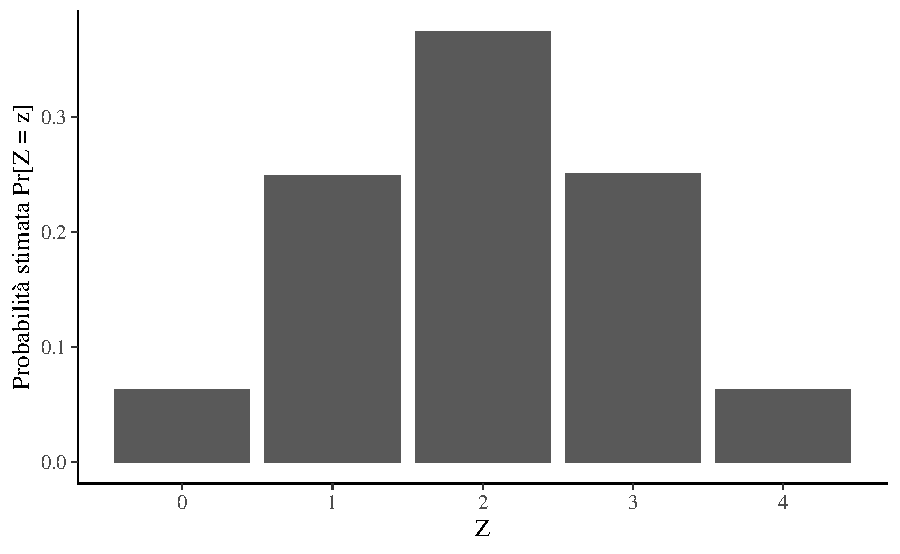
\includegraphics{ds4psy_files/figure-latex/barplot-mdf-4coins-1} 

}

\caption{Grafico di $M = 100\,000$ simulazioni della funzione di massa di probabilità di una variabile casuale definita come il numero di teste in quattro lanci di una moneta equilibrata.}\label{fig:barplot-mdf-4coins}
\end{figure}

Se \(A\) è un sottoinsieme della variabile casuale \(Z\), allora denotiamo con \(P_{z}(A)\) la probabilità assegnata ad \(A\) dalla distribuzione \(P_{z}\). Mediante una distribuzione di probabilità \(P_{z}\) è dunque possibile determinare la probabilità di ciascun sottoinsieme \(A \subset Z\) come

\[
P_{z}(A) = \sum_{z \in A} P_{z}(Z).
\]

\begin{example}
Nel caso dell'esempio discusso nella Sezione \ref{sec:fun-mass-prob}, la probabilità che la variabile casuale \(Z\) sia un numero dispari è

\[
P(\text{Z è un numero dispari}) = P_{z}(Z = 1) + P_{z}(Z = 3) = \frac{4}{16} + \frac{4}{16} = \frac{1}{2}.
\]
\end{example}

\hypertarget{commenti-e-considerazioni-finali}{%
\section*{Commenti e considerazioni finali}\label{commenti-e-considerazioni-finali}}


In questo capitolo abbiamo visto come si costruisce lo spazio campione di un esperimento casuale, quali sono le proprietà di base della probabilità e come si assegnano le probabilità agli eventi definiti sopra uno spazio campione discreto. Abbiamo anche introdotto le nozioni di ``variabile casuale'', ovvero di una variabile che prende i suoi valori casualmente. E abbiamo descritto il modo di specificare la probabilità con cui sono presi i differenti valori, ovvero la funzione di distribuzione probabilistica \(F(X) = P(X < x)\), e la funzione di massa di probabilità. Le procedure di analisi dei dati psicologici che discuteremo in seguito faranno un grande uso di questi concetti e della notazione qui introdotta.

\hypertarget{chapter-prob-cond}{%
\chapter{Probabilità condizionata}\label{chapter-prob-cond}}

Il fondamento della statistica bayesiana è il teorema di Bayes e il teorema di Bayes è una semplice ridescrizione della probabilità condizionata. Esaminiamo dunque la probabilità condizionata.

\hypertarget{sec:bayes-cancer}{%
\section{Probabilità condizionata su altri eventi}\label{sec:bayes-cancer}}

L'attribuzione di una probabilità ad un evento è sempre condizionata dalle conoscenze che abbiamo a disposizione. Per un determinato stato di conoscenze, attribuiamo ad un dato evento una certa probabilità di verificarsi; ma se il nostro stato di conoscenze cambia, allora cambierà anche la probabilità che attribuiremo all'evento in questione. Infatti, si può pensare che tutte le probabilità siano probabilità condizionate, anche se l'evento condizionante non è sempre esplicitamente menzionato.

Per introdurre la probabilità condizionata, \citet{albert2019probability} utilizzando il famoso paradosso delle tre carte. ``Ci sono tre carte, delle quali la prima (A) è rossa su entrambi i lati, la seconda (B) su un lato è rossa e sull'altro è bianca e la terza (C) è bianca su entrambi i lati. Ponendo su un tavolo una delle tre carte, scelta a caso, ottengo che il lato visibile è di colore rosso. Qual è la probabilità che anche il lato non visibile sia di colore rosso? La risposta intuitiva porta solitamente a rispondere che la probabilità ricercata sia pari al 50\%, in quanto solo due carte (la A e la B) possono mostrare il colore rosso e solo una di queste (la A) può mostrare anche sull'altro lato il colore rosso; tuttavia si dimostra che la risposta giusta è 2/3.'' (da Wikipedia)

\citet{albert2019probability} propongono di risolvere il problema con una simulazione in \(\textsf{R}\): prima di tutto si sceglie una carta a caso, e poi si sceglie un lato della carta. Ci sono tre carte possibili, che chiamiamo ``c\_rossa'', ``c\_bianca'', e ``c\_entrambi''. Per la carta rossa, ci sono due lati rossi; per la carta bianca ci sono due lati bianchi e la carta ``entrambi'' ha un lato rosso e un lato bianco. Ripetiamo l'esperimento 1,000 volte e classifichiamo i risultati per tipo di carta e lato:

\begin{Shaded}
\begin{Highlighting}[]
\FunctionTok{set.seed}\NormalTok{(}\DecValTok{84735}\NormalTok{)}
\NormalTok{df }\OtherTok{\textless{}{-}} \FunctionTok{tibble}\NormalTok{(}
  \AttributeTok{Carta =} \FunctionTok{c}\NormalTok{(}
    \StringTok{"c\_rossa"}\NormalTok{, }\StringTok{"c\_rossa"}\NormalTok{, }\StringTok{"c\_bianca"}\NormalTok{, }\StringTok{"c\_bianca"}\NormalTok{, }\StringTok{"c\_entrambi"}\NormalTok{,}
    \StringTok{"c\_entrambi"}
\NormalTok{  ),}
  \AttributeTok{Lato =} \FunctionTok{c}\NormalTok{(}
    \StringTok{"rosso"}\NormalTok{, }\StringTok{"rosso"}\NormalTok{, }\StringTok{"bianco"}\NormalTok{, }\StringTok{"bianco"}\NormalTok{, }\StringTok{"rosso"}\NormalTok{, }\StringTok{"bianco"}
\NormalTok{  )}
\NormalTok{)}
\NormalTok{df}
\CommentTok{\#\textgreater{} \# A tibble: 6 x 2}
\CommentTok{\#\textgreater{}   Carta      Lato  }
\CommentTok{\#\textgreater{}   \textless{}chr\textgreater{}      \textless{}chr\textgreater{} }
\CommentTok{\#\textgreater{} 1 c\_rossa    rosso }
\CommentTok{\#\textgreater{} 2 c\_rossa    rosso }
\CommentTok{\#\textgreater{} 3 c\_bianca   bianco}
\CommentTok{\#\textgreater{} 4 c\_bianca   bianco}
\CommentTok{\#\textgreater{} 5 c\_entrambi rosso }
\CommentTok{\#\textgreater{} 6 c\_entrambi bianco}
\NormalTok{carte }\OtherTok{\textless{}{-}} \FunctionTok{sample\_n}\NormalTok{(df, }\DecValTok{1000}\NormalTok{, }\AttributeTok{replace =} \ConstantTok{TRUE}\NormalTok{)}
\FunctionTok{table}\NormalTok{(carte}\SpecialCharTok{$}\NormalTok{Carta, carte}\SpecialCharTok{$}\NormalTok{Lato)}
\CommentTok{\#\textgreater{}             }
\CommentTok{\#\textgreater{}              bianco rosso}
\CommentTok{\#\textgreater{}   c\_bianca      353     0}
\CommentTok{\#\textgreater{}   c\_entrambi    143   160}
\CommentTok{\#\textgreater{}   c\_rossa         0   344}
\end{Highlighting}
\end{Shaded}

Se si osserva il colore rosso (seconda colonna nella tabella precedente), questo risultato è dovuto ad una carta rossa in 344 casi e ad una carta ``entrambi'' in 160 casi. Quindi, nella simulazione il colore rosso (344 + 160) è associato ad una carta rossa in circa 2/3 dei casi -- ciò significa che, se i lato visibile è di colore rosso, allora c'è una probabilità di 2/3 che anche il lato non visibile sia di colore rosso. Questo esempio dimostra come le nostre intuizioni a proposito della probabilità condizionata non sono sempre corrette. Consideriamo un altro problema più articolato.

\begin{exercise}

Supponiamo che lo screening per la diagnosi precoce del tumore mammario si avvalga di test che sono accurati al 90\%, nel senso che il 90\% delle donne con cancro e il 90\% delle donne senza cancro saranno classificate correttamente. Supponiamo che l'1\% delle donne sottoposte allo screening abbia effettivamente il cancro al seno. Ci chiediamo: qual è la probabilità che una donna scelta casualmente abbia una mammografia positiva e, se ce l'ha, qual è la probabilità che abbia davvero il cancro?

Per risolvere questo problema, supponiamo che il test in questione venga somministrato ad un grande campione di donne, diciamo a 1000 donne. Di queste 1000 donne, 10 (ovvero, l'1\%) hanno il cancro al seno. Per queste 10 donne, il test darà un risultato positivo in 9 casi (ovvero, nel 90\% dei casi). Per le rimanenti 990 donne che non hanno il cancro al seno, il test darà un risultato positivo in 99 casi (se la probabilità di un vero positivo è del 90\%, la probabilità di un falso positivo è del 10\%). Questa situazione è rappresentata nella figura \ref{fig:mammografia}.

Combinando i due risultati precedenti, vediamo che il test dà un risultato positivo per 9 donne che hanno effettivamente il cancro al seno e per 99 donne che non ce l'hanno, per un totale di 108 risultati positivi. Dunque, la probabilità di ottenere un risultato positivo al test è \(\frac{108}{1000}\) = 11\%. Ma delle 108 donne che hanno ottenuto un risultato positivo al test, solo 9 hanno il cancro al seno. Dunque, la probabilità di avere il cancro, dato un risultato positivo al test, è pari a \(\frac{9}{108}\) = 8\%.

\begin{figure}

{\centering 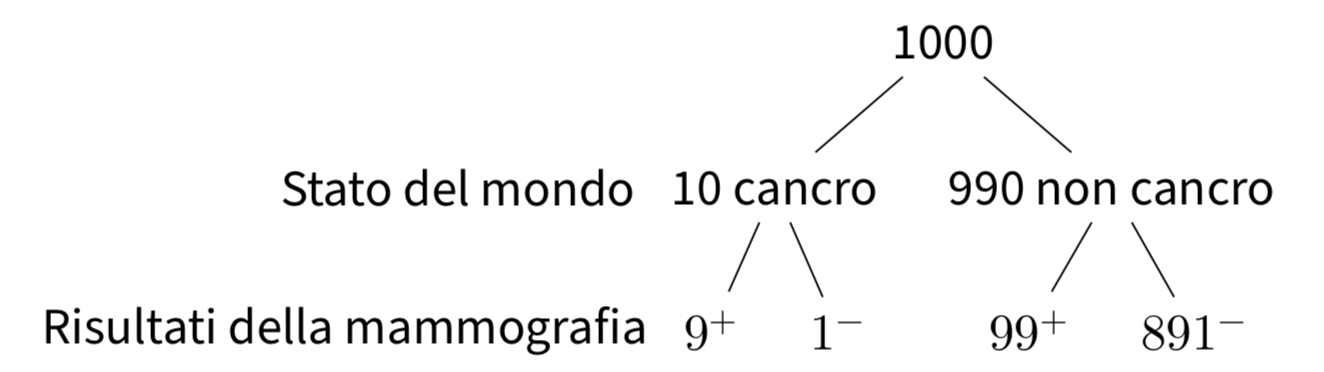
\includegraphics[width=0.77\linewidth]{images/mammografia} 

}

\caption{Rappresentazione ad albero che riporta le frequenze attese dei risultati di una mammografia in un campione di 1,000 donne.}\label{fig:mammografia}
\end{figure}

\end{exercise}

Nell'esercizio precedente, la probabilità dell'evento ``ottenere un risultato positivo al test'' è una probabilità non condizionata, mentre la probabilità dell'evento ``avere il cancro al seno, dato che il test ha prodotto un risultato positivo'' è una probabilità condizionata.

In termini generali, la probabilità condizionata \(P(A \mid B)\) rappresenta la probabilità che si verifichi l'evento \(A\) sapendo che si è verificato l'evento \(B\). Ciò ci conduce alla seguente definizione.

\begin{definition}
Dato un qualsiasi evento \(A\), si chiama \emph{probabilità condizionata} di \(A\) dato \(B\) il numero

\begin{equation}
P(A \mid B) = \frac{P(A \cap B)}{P(B)}, \quad \text{con}\, P(B) > 0,
\label{eq:probcond}
\end{equation}

dove \(P(A\cap B)\) è la \emph{probabilità congiunta} dei due eventi, ovvero la probabilità che si verifichino entrambi.
\end{definition}

Concludiamo con un problema veramente semplice per consolidare la nostra comprensione del concetto di probabilità condizionata.

\begin{exercise}
Da un mazzo di 52 carte (13 carte per ciascuno dei 4 semi) ne viene estratta una in modo casuale. Qual è la probabilità che esca una figura di cuori? Sapendo che la carta estratta ha il seme di cuori, qual è la probabilità che il valore numerico della carta sia 7, 8 o 9?

Ci sono 13 carte di cuori, dunque la risposta alla prima domanda è 1/4 (probabilità non condizionata). Per rispondere alla seconda domanda consideriamo solo le 13 carte di cuori; la probabilità cercata è dunque 3/13 (probabilità condizionata).
\end{exercise}

\hypertarget{la-regola-moltiplicativa}{%
\section{La regola moltiplicativa}\label{la-regola-moltiplicativa}}

Dalla definizione di probabilità condizionata è possibile esprimere la probabilità congiunta tramite le condizionate. La regola moltiplicativa (o legge delle probabilità composte, o regola della catena) afferma che la probabilità che si verifichino due eventi \(A\) e \(B\) è pari alla probabilità di uno dei due eventi moltiplicato con la probabilità dell'altro evento condizionato al verificarsi del primo:

\begin{equation}
P(A \cap B) = P(B)P(A \mid B) = P(A)P(B \mid A).
\label{eq:probcondinv}
\end{equation}

La \eqref{eq:probcondinv} si estende al caso di \(n\) eventi \(A_1, \dots, A_n\) nella forma seguente:

\begin{equation}
P\left( \bigcap_{k=1}^n A_k \right) = \prod_{k=1}^n \left(  A_k  \ \Biggl\lvert \ \bigcap_{j=1}^{k-1} A_j \right)
\label{eq:probcomposte}
\end{equation}

Per esempio, nel caso di quattro eventi abbiamo

\begin{equation}
\begin{split}
P(A_1 \cap A_2 \cap A_3 \cap A_4) = {}& P(A_1) \cdot P(A_2 \mid A_1) \cdot  P(A_3 \mid A_1 \cap A_2) \cdot \\
 & P(A_4 \mid A_1 \cap A_2 \cap A_{3}).\notag
\end{split}
\end{equation}

\begin{exercise}
Da un'urna contenente 6 palline bianche e 4 nere si estrae una pallina per volta, senza reintrodurla nell'urna. Indichiamo con \(B_i\) l'evento: ``esce una pallina bianca alla \(i\)-esima estrazione'' e con \(N_i\) l'estrazione di una pallina nera. L'evento: ``escono due palline bianche nelle prime due estrazioni'' è rappresentato dalla intersezione \(\{B_1 \cap B_2\}\) e la sua probabilità vale, per la \eqref{eq:probcondinv}

\[
P(B_1 \cap B_2) = P(B_1)P(B_2 \mid B_1).
\]

\(P(B_1)\) vale 6/10, perché nella prima estrazione \(\Omega\) è costituito da 10 elementi: 6 palline bianche e 4 nere. La probabilità condizionata \(P(B_2 \mid B_1)\) vale 5/9, perché nella seconda estrazione, se è verificato l'evento \(B_1\), lo spazio campionario consiste di 5 palline bianche e 4 nere. Si ricava pertanto:

\[
P(B_1 \cap B_2) = \frac{6}{10} \cdot \frac{5}{9} = \frac{1}{3}.
\]

In modo analogo si ha che

\[
P(N_1 \cap N_2) = P(N_1)P(N_2 \mid N_1) = \frac{4}{10} \cdot \frac{3}{9} = \frac{4}{30}.
\]

Se l'esperimento consiste nell'estrazione successiva di 3 palline, la probabilità che queste siano tutte bianche vale, per la \eqref{eq:probcomposte}:

\[
P(B_1 \cap B_2 \cap B_3)=P(B_1)P(B_2 \mid B_1)P(B_3 \mid B_1 \cap B_2),
\]

dove la probabilità \(P(B_3 \mid B_1 \cap B_2)\) si calcola supponendo che si sia verificato l'evento condizionante \(\{B_1 \cap B_2\}\). Lo spazio campionario per questa probabilità condizionata è costituito da 4 palline bianche e 4 nere, per cui \(P(B_3 \mid B_1 \cap B_2) = 1/2\) e quindi:

\[
P (B_1 \cap B_2 \cap B_3) = \frac{6}{10}\cdot\frac{5}{9} \cdot\frac{4}{8}  = \frac{1}{6}.
\]

La probabilità dell'estrazione di tre palline nere è invece:

\[
\begin{aligned}
P(N_1 \cap N_2 \cap N_3) &= P(N_1)P(N_2 \mid N_1)P(N_3 \mid N_1 \cap N_2)\notag\\ 
&= \frac{4}{10} \cdot \frac{3}{9} \cdot \frac{2}{8} = \frac{1}{30}.\notag
\end{aligned}
\]
\end{exercise}

\hypertarget{lindipendendenza-stocastica}{%
\section{L'indipendendenza stocastica}\label{lindipendendenza-stocastica}}

Un concetto molto importante per le applicazioni statistiche della probabilità è quello dell'indipendenza stocastica. La definizione \eqref{eq:probcond} consente di esprimere il concetto di indipendenza di un evento da un altro in forma intuitiva: se \(A\) e \(B\) sono eventi indipendenti, allora il verificarsi di \(A\) non influisce sulla probabilità del verificarsi di \(B\), ovvero non la condiziona, e il verificarsi di \(B\) non influisce sulla probabilità del verificarsi di \(A\). Infatti, per la \eqref{eq:probcond}, si ha che, se \(A\) e \(B\) sono due eventi indipendenti, risulta:

\[
P(A \mid B) = \frac{P(A)P(B)}{P(B)} = P(A),
\]

\[
P(B \mid A) = \frac{P(A)P(B)}{P(A)} = P(B).
\]

Possiamo dunque dire che due eventi \(A\) e \(B\) sono indipendenti se

\begin{equation}
\begin{split}
P(A \mid B) &= P(A), \\
P(B \mid A) &= P(B).
\end{split}
\end{equation}

\hypertarget{il-teorema-della-probabilituxe0-totale}{%
\section{Il teorema della probabilità totale}\label{il-teorema-della-probabilituxe0-totale}}

Dato un insieme finito \(A_i\) di eventi, nel calcolo della probabilità dell'unione di tutti gli eventi, se gli eventi considerati non sono a due a due incompatibili, si deve tenere conto delle loro intersezioni. In particolare, la probabilità dell'unione di due eventi \(A\) e \(B\) è pari alla somma delle singole probabilità \(P(A)\) e \(P(B)\) diminuita della probabilità della loro intersezione:

\begin{equation}
P(A \cup B) = P(A) + P(B) - P(A \cap B).
\label{eq:probunione}
\end{equation}

Nel caso di tre eventi, si ha

\[
\begin{split}
P(A \cup B \cup C) &= P(A)+P(B)+P(C)-P(A\cap B)-P(A\cap C) - \\
& \qquad P(B\cap C) + P(A\cap B\cap C).
\end{split}
\]

La formula per il caso di \(n\) eventi si ricava per induzione.

Per il caso di due soli eventi, se \(A\) e \(B\) sono indipendenti, la \eqref{eq:probunione} si modifica nella relazione seguente:

\begin{equation}
P(A \cup B) = P(A) + P(B) - P(A)P(B).
\end{equation}

Nel caso di due eventi \(A\) e \(B\) incompatibili, se cioè \(P(A \cap B) = \varnothing\), si ha che

\[
A\cap B=\varnothing \Rightarrow P(A\cup B)=P(A)+P(B).
\]

Si può dimostrare per induzione che ciò vale anche per un insieme finito di eventi \(A_{n}\) a due a due incompatibili, ovvero che:

\[
A_i\cap A_j=\varnothing, i\neq j \Rightarrow P\left(\bigcup_{i=1}^n A_i\right)=\sum_{i=1}^nP(A_i).
\]

\begin{exercise}
Nel lancio di due dadi non truccati, si considerino gli eventi: \emph{A} = \{esce un 1 o un 2 nel primo lancio\} e \emph{B} = \{il punteggio totale è 8\}. Gli eventi \emph{A} e \emph{B} sono indipendenti?

Rappresentiamo qui sotto lo spazio campionario dell'esperimento casuale.

\begin{figure}

{\centering 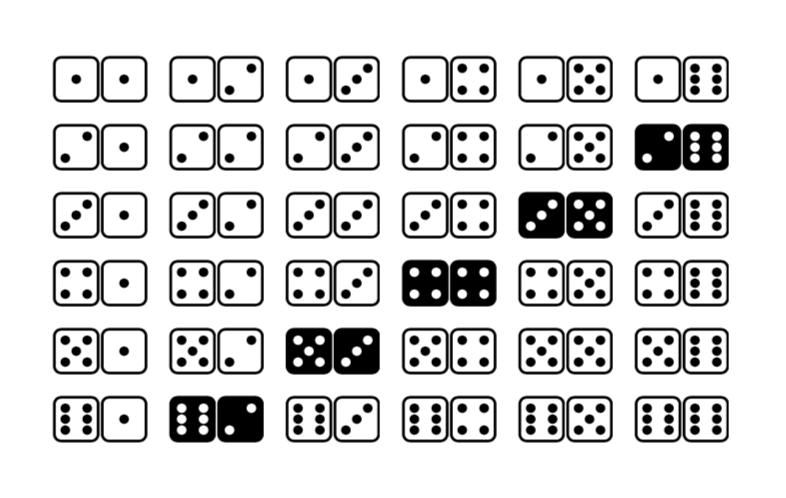
\includegraphics[width=0.7\linewidth]{images/sampling-space-dice} 

}

\caption{Rappresentazione dello spazio campionario dei risultati dell'esperimento casuale corrispondente al lancio di due dadi bilanciati. Sono evidenziati gli eventi elementari che costituiscono l'evento A: esce un 1 o un 2 nel primo lancio.}\label{fig:sampling-space-dice}
\end{figure}

Gli eventi \emph{A} e \emph{B} non sono statisticamente indipendenti. Infatti, le loro probabilità valgono \emph{P}(A) = 12/36 e \emph{P}(B) = 5/36 e la probabilità della loro intersezione è

\[
P(A \cap B) = 1/36 = 3/108 \neq P(A)P(B) = 5/108.
\]
\end{exercise}

\begin{remark}
Il concetto di indipendenza è del tutto differente da quello di incompatibilità. Si noti infatti che due eventi \emph{A} e \emph{B} incompatibili (per i quali si ha \(A \cap B = \emptyset\)) sono statisticamente dipendenti, poiché il verificarsi dell'uno esclude il verificarsi dell'altro: \(P(A \cap B)=0 \neq P(A)P(B)\).
\end{remark}

\hypertarget{il-teorema-della-probabilituxe0-assoluta}{%
\section{Il teorema della probabilità assoluta}\label{il-teorema-della-probabilituxe0-assoluta}}

Il teorema della probabilità assoluta consente di calcolare la probabilità di un evento \(E\) di cui sono note le probabilità condizionate rispetto ad altri eventi \((H_i)_{i\geq 1}\), a condizione che essi costituiscano una partizione dell'evento certo \(\Omega\), ovvero

\begin{enumerate}
\def\labelenumi{\arabic{enumi}.}
\tightlist
\item
  \(\bigcup_{i=1}^\infty H_i = \Omega\);
\item
  \(H_j \cap H_j = \emptyset, i\neq j\);
\item
  \(P(H_i) > 0, i = 1, \dots, \infty\).
\end{enumerate}

Nel caso di una partizione dello spazio campione in \(n\) sottoinsiemi abbiamo

\begin{equation}
{\mbox{P}}(E)=\sum _{{i=1}}^{n}{\mbox{P}}(H_{i}\cap E)=\sum _{{i=1}}^{n}{\mbox{P}}(H_{i}){\mbox{P}}(E \mid H_{i}).
\end{equation}

Consideriamo, ad esempio, una partizione dell'evento certo in tre soli sottoinsiemi.

\begin{figure}

{\centering 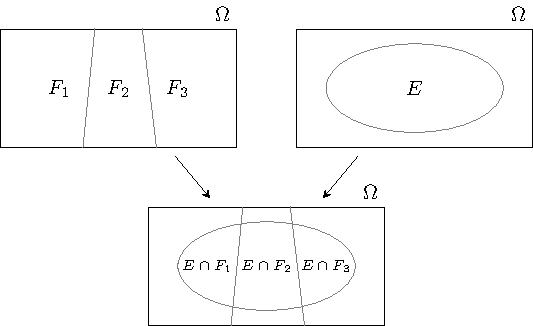
\includegraphics{ds4psy_files/figure-latex/tikz-prob-tot-1} 

}

\caption{Partizione dell'evento certo $\Omega$ in tre sottoinsiemi sui quali viene definito l'evento $E$.}\label{fig:tikz-prob-tot}
\end{figure}

In tali circostanze si ha che

\begin{equation}
{\mbox{P}}(E) = {\mbox{P}}(E \cap H_1) + {\mbox{P}}(E \cap H_2) + {\mbox{P}}(E \cap H_3), \notag
\label{eq:prob-total-1a}
\end{equation}

ovvero

\begin{equation}
{\mbox{P}}(E) = {\mbox{P}}(E \mid H_1) {\mbox{P}}(H_1) + {\mbox{P}}(E \mid H_2) {\mbox{P}}(H_2) + {\mbox{P}}(E \mid H_3) {\mbox{P}}(H_3).
\label{eq:prob-total-1b}
\end{equation}

In base al teorema della probabilità assoluta, dunque, se l'evento \(E\) è costituito da tutti gli eventi elementari in \(E \cap H_1\), \(E \cap H_2\) e \(E \cap H_3\), allora la sua probabilità è data dalla somma delle probabilità condizionate \(P(E \mid H_i)\), ciascuna delle quali pesata per la probabilità dell'evento condizionante \(H_i\).

\begin{exercise}
Si considerino tre urne, ciascuna delle quali contiene 100 palline:

\begin{itemize}
\tightlist
\item
  Urna 1: 75 palline rosse e 25 palline blu,
\item
  Urna 2: 60 palline rosse e 40 palline blu,
\item
  Urna 3: 45 palline rosse e 55 palline blu.
\end{itemize}

\noindent Una pallina viene estratta a caso da un'urna anch'essa scelta a caso. Qual è la probabilità che la pallina estratta sia di colore rosso?

Sia \(R\) l'evento ``la pallina estratta è rossa'' e sia \(U_i\) l'evento che corrisponde alla scelta dell'\(i\)-esima urna. Sappiamo che

\[
{\mbox{P}}(R \mid U_1) = 0.75, \quad {\mbox{P}}(R \mid U_2) = 0.60, \quad {\mbox{P}}(R \mid U_3) = 0.45.
\]

Gli eventi \(U_1\), \(U_2\) e \(U_3\) costituiscono una partizione dello spazio campionario in quanto \(U_1\), \(U_2\) e \(U_3\) sono eventi mutualmente esclusivi ed esaustivi, \({\mbox{P}}(U_1 \cup U_2 \cup U_3) = 1.0\). In base al teorema della probabilità assoluta, la probabilità di estrarre una pallina rossa è dunque

\[
\begin{split}
{\mbox{P}}(R) &= {\mbox{P}}(R \mid U_1){\mbox{P}}(U_1)+{\mbox{P}}(R \mid U_2){\mbox{P}}(U_2)+{\mbox{P}}(R \mid U_3){\mbox{P}}(U_3) \\
&= 0.75 \cdot \frac{1}{3}+0.60 \cdot \frac{1}{3}+0.45 \cdot \frac{1}{3} \\
&=0.60.
\end{split}
\]
\end{exercise}

\hypertarget{indipendenza-condizionale}{%
\section{Indipendenza condizionale}\label{indipendenza-condizionale}}

Aggiungo qui delle considerazioni sul concetto di indipendenza condizionale a cui si farà riferimento nell'ultima parte della dispensa. L'indipendenza condizionale descrive situazioni in cui un'osservazione è irrilevante o ridondante quando si valuta la certezza di un'ipotesi. L'indipendenza condizionale è solitamente formulata nei termini della probabilità condizionata, come un caso speciale in cui la probabilità dell'ipotesi data un'osservazione non informativa è uguale alla probabilità senza tale osservazione non informativa.

Se \(A\) è l'ipotesi e \(B\) e \(C\) sono osservazioni, l'indipendenza condizionale può essere espressa come l'uguaglianza:

\[
P(A \mid B,C)=P(A \mid C).
\]

Dato che \(P(A \mid B,C)\) è uguale a \(P(A \mid C)\), questa uguaglianza corrisponde all'affermazione che \(B\) non fornisce alcun contributo alla certezza di \(A\). In questo caso si dice che \(A\) e \(B\) condizionalmente indipendente dato \(C\), scritto simbolicamente come: \((A \perp\!\!\!\!\perp B \mid C)\).

In maniera equivalente, l'indipendenza condizionale \((A \perp\!\!\!\!\perp B \mid C)\) si verifica se:

\[
P(A, B \mid C) = P(A \mid C) P(B \mid C).
\]

Un esempio è il seguente (da Wikipedia). Siano due eventi le probabilità che le persone A e B tornino a casa in tempo per la cena, e il terzo evento è il fatto che una tempesta di neve ha colpito la città. Mentre sia A che B hanno una probabilità più piccola di tornare a casa in tempo per cena (di quando non c'è la neve), tali probabilità sono comunque indipendenti l'una dall'altra. Cioè, sapere che A è in ritardo non ci dice nulla sul fatto che B sia in ritardo o meno. (A e B potrebbero vivere in quartieri diversi, percorrere distanze diverse e utilizzare mezzi di trasporto diversi.) Tuttavia, se sapessimo che A e B vivono nello stesso quartiere, usano lo stesso mezzo di trasporto e lavorano nello stesso luogo, allora i due eventi non sarebbero condizionatamente indipendenti.

\hypertarget{commenti-e-considerazioni-finali-1}{%
\section*{Commenti e considerazioni finali}\label{commenti-e-considerazioni-finali-1}}


La probabilità condizionata è importante perché ci fornisce uno strumento per precisare il concetto di indipendenza statistica. Una delle domande più importanti delle analisi statistiche è infatti quella che si chiede se due variabili sono associate tra loro oppure no. In questo Capitolo abbiamo discusso il concetto di indipendenza (come contrapposto al concetto di associazione -- si veda il Capitolo \ref{chapter-descript}). In seguito vedremo come sia possibile fare inferenza sull'associazione tra variabili.

\hypertarget{chapter-teo-bayes}{%
\chapter{Il teorema di Bayes}\label{chapter-teo-bayes}}

Il teorema di Bayes assume un ruolo fondamentale nell'interpretazione soggettivista della probabilità perché descrive l'aggiornamento della fiducia che si aveva nel verificarsi di una determinata ipotesi \(H\) (identificata con la probabilità assegnata all'ipotesi stessa) in conseguenza del verificarsi dell'evidenza \(E\).

\hypertarget{il-teorema-di-bayes}{%
\section{Il teorema di Bayes}\label{il-teorema-di-bayes}}

\begin{theorem}
Sia \((H_i)_{i\geq 1}\) una partizione dell'evento certo \(\Omega\) e sia \(E \subseteq \Omega\) un evento tale che \(p(E) > 0\), allora, per \(i = 1, \dots, \infty\):

\begin{equation}
{\mbox{P}}(H_i \mid E) = \frac{{\mbox{P}}(E \mid H_i){\mbox{P}}(H_i)}{\sum_{j=1}^{\infty}{\mbox{P}}(H_j)P(E \mid H_j)}.
\label{eq:bayes2}
\end{equation}
\end{theorem}

La formula di Bayes contiene tre concetti fondamentali. I primi due distinguono il grado di fiducia precedente al verificarsi dell'evidenza \(E\) da quello successivo al verificarsi dell'evidenza \(E\). Pertanto, dati gli eventi \(H, E \subseteq \Omega\)

\begin{itemize}
\tightlist
\item
  si definisce \emph{probabilità a priori} la probabilità che viene attribuita al verificarsi di \(H\) prima di sapere che si è verificato l'evento \(E\), seguendo l'approccio bayesiano, ovvero tenendo conto delle caratteristiche cognitive del decisore (esperienza, modo di pensare, ecc.);
\item
  si definisce \emph{probabilità a posteriori} la probabilità assegnata ad \(H\), una volta che sia noto \(E\), ovvero l'aggiornamento della probabilità a priori alla luce della nuova evidenza \(E\).
\end{itemize}

Il terzo concetto definisce la probabilità che ha l'evento \(E\) di verificarsi quando è vera l'ipotesi \(H\), ovvero la probabilità dell'evidenza in base all'ipotesi. Pertanto, dati gli eventi \(H, E \subseteq \Omega\)

\begin{itemize}
\tightlist
\item
  si definisce \emph{verosimiglianza} di \(H\) dato \(E\), la probabilità condizionata che si verifichi \(E\), se è vera \(H\): \(P (E \mid H)\).
\end{itemize}

Si noti che per il calcolo della quantità a denominatore si ricorre al teorema della probabilità assoluta.

Per fare un esempio concreto, considerando una partizione dell'evento certo \(\Omega\) in due soli eventi che chiamiamo ipotesi \(H_1\) e \(H_2\). Supponiamo conosciute le probabilità a priori \(P(H_1)\) e \(P(H_2)\). Consideriamo un terzo evento \(E \subseteq \Omega\) con probabilità non nulla di cui si conosce la verosimiglianza, ovvero si conoscono le probabilità condizionate \({\mbox{P}}(E \mid H_1)\) e \(P(E \mid H_2)\). Supponendo che si sia verificato l'evento \(E\), vogliamo conoscere le probabilità a posteriori delle ipotesi, ovvero \(P(H_1 \mid E)\) e \(P(H_2 \mid E)\).

\begin{figure}

{\centering 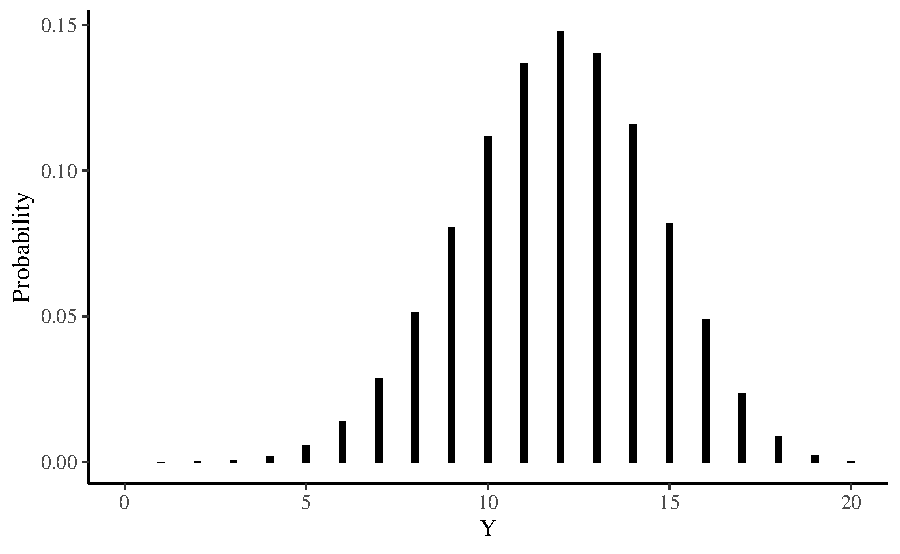
\includegraphics[width=0.45\linewidth]{ds4psy_files/figure-latex/unnamed-chunk-18-1} 

}

\end{figure}

Per trovare le probabilità cercate scriviamo:

\[
\begin{split}
{\mbox{P}}(H_1 \mid E) &= \frac{{\mbox{P}}(E \cap H_1)}{{\mbox{P}}(E)}\notag\\
              &= \frac{{\mbox{P}}(E \mid H_1){\mbox{P}}(H_1)}{{\mbox{P}}(E)}.
\end{split}
\]

Sapendo che \(E = (E \cap H_1) \cup (E \cap H_2)\) e che \(H_1\) e \(H_2\) sono eventi disgiunti, ovvero \(H_1 \cap H_2 = \emptyset\), ne segue che possiamo calcolare \({\mbox{P}}(E)\) utilizzando il teorema della probabilità assoluta:

\[
\begin{split}
{\mbox{P}}(E) &= {\mbox{P}}(E \cap H_1) + {\mbox{P}}(E \cap H_2)\notag\\
     &= {\mbox{P}}(E \mid H_1)P(H_1) + {\mbox{P}}(E \mid H_2){\mbox{P}}(H_2).
\end{split}
\]

\noindent Sostituendo tale risultato nella formula precedente otteniamo:

\begin{equation}
{\mbox{P}}(H_1 \mid E) = \frac{{\mbox{P}}(E \mid H_1){\mbox{P}}(H_1)}{{\mbox{P}}(E \mid H_1){\mbox{P}}(H_1) + {\mbox{P}}(E \mid H_2)P(H_2)}.
\label{eq:bayes1}
\end{equation}

Un lettore attento si sarà reso conto che, in precedenza, abbiamo già applicato il teorema di Bayes quando abbiamo risolto l'esercizio riportato nella Sezione \ref{sec:bayes-cancer}. In quel caso, le due ipotesi erano ``malattia presente'', che possiamo denotare con \(M\), e ``malattia assente'', \(M^\complement\). L'evidenza \(E\) è costituita dal risultato positivo al test, ovvero \(+\). Con questa nuova notazione la \eqref{eq:bayes1} diventa:

\begin{equation}
{\mbox{P}}(M \mid +) = \frac{{\mbox{P}}(+ \mid M) {\mbox{P}}(M)}{{\mbox{P}}(+ \mid M) {\mbox{P}}(M) + {\mbox{P}}(+ \mid M^\complement) {\mbox{P}}(M^\complement)}\notag
\end{equation}

Inserendo i dati nella formula, otteniamo

\begin{align}
{\mbox{P}}(M \mid +) &= \frac{0.9 \cdot 10/1000}{0.9 \cdot 10/1000 + 99 / 990 \cdot 990 / 1000} \notag\\
&= \frac{9}{108}.\notag
\end{align}

\hypertarget{commenti-e-considerazioni-finali-2}{%
\section*{Commenti e considerazioni finali}\label{commenti-e-considerazioni-finali-2}}


Il teorema di Bayes rende esplicito il motivo per cui la probabilità non possa essere pensata come uno stato oggettivo, quanto piuttosto come un'inferenza soggettiva e condizionata. Il denominatore del membro di destra della \eqref{eq:bayes2} è un semplice fattore di normalizzazione. Nel numeratore compaiono invece due quantità: \({\mbox{P}}(H_i\)) e \({\mbox{P}}(E \mid H_i)\). La probabilità \({\mbox{P}}(H_i\)) è la probabilità \emph{probabilità a priori} (\emph{prior}) dell'ipotesi \(H_i\) e rappresenta l'informazione che l'agente bayesiano possiede a proposito dell'ipotesi \(H_i\). Diremo che \({\mbox{P}}(H_i)\) codifica il grado di fiducia che l'agente ripone in \(H_i\) precedentemente al verificarsi dell'evidenza \(E\). Nell'interpretazione bayesiana, \({\mbox{P}}(H_i)\) rappresenta un giudizio personale dell'agente e non esistono criteri esterni che possano determinare se tale giudizio sia coretto o meno. La probabilità condizionata \({\mbox{P}}(E \mid H_i)\) rappresenta invece la verosimiglianza di \(H_i\) dato \(E\) e descrive la plausibilità che si verifichi l'evento \(E\) se è vera l'ipotesi \(H_i\). Il teorema di Bayes descrive la regola che l'agente deve seguire per aggiornare il suo grado di fiducia nell'ipotesi \(H_i\) alla luce del verificarsi dell'evento \(E\). La \({\mbox{P}}(H_i \mid E)\) è chiamata probabilità a posteriori dato che rappresenta la nuova probabilità che l'agente assegna all'ipotesi \(H_i\) affinché rimanga consistente con le nuove informazioni fornitegli da \(E\).

La probabilità a posteriori dipende sia dall'evidenza \(E\), sia dalla conoscenza a priori dell'agente \({\mbox{P}}(H_i)\). È dunque chiaro come non abbia senso parlare di una probabilità oggettiva: per il teorema di Bayes la probabilità è definita condizionatamente alla probabilità a priori, la quale a sua volta, per definizione, è un'assegnazione soggettiva. Ne segue pertanto che ogni probabilità deve essere considerata come una rappresentazione del grado di fiducia soggettiva dell'agente. Dato che ogni assegnazione probabilistica rappresenta uno stato di conoscenza e che ciascun particolare stato di conoscenza è arbitrario, un accordo tra agenti diversi non è richiesto. Tuttavia, la teoria delle probabilità ci fornisce uno strumento che, alla luce di nuove evidenze, consente di aggiornare in un modo razionale il grado di fiducia che attribuiamo ad un'ipotesi, via via che nuove evidenze vengono raccolte, in modo tale da formulare un'ipotesi a posteriori la quale non è mai definitiva, ma può sempre essere aggiornata in base alle nuove evidenze disponibili. Questo processo si chiama \emph{aggiornamento bayesiano}. Vedremo nel Capitolo \ref{ch:intro-bayes-inference} come estendere la \eqref{eq:bayes2} al caso continuo.

\hypertarget{chapter-prob-congiunta}{%
\chapter{Probabilità congiunta}\label{chapter-prob-congiunta}}

La probabilità congiunta è la probabilità che due o più eventi si verifichino contemporaneamente. In questo Capitolo verrà esaminato in dettaglio il caso discreto.

\hypertarget{funzione-di-probabilituxe0-congiunta}{%
\section{Funzione di probabilità congiunta}\label{funzione-di-probabilituxe0-congiunta}}

Dopo aver trattato della distribuzione di probabilità di una variabile casuale, la quale associa ad ogni evento elementare dello spazio campionario uno ed un solo numero reale, è naturale estendere questo concetto al caso di due o più variabili casuali.

Iniziamo a descrivere il caso discreto con un esempio. Consideriamo l'esperimento casuale corrispondente al lancio di tre monete equilibrate. Lo spazio campionario è

\[
\Omega = \{TTT, TTC, TCT, CTT, CCT, CTC, TCC, CCC\}.
\]

Dato che i tre lanci sono tra loro indipendenti, non c'è ragione di aspettarsi che uno degli otto risultati possibili dell'esperimento sia più probabile degli altri, dunque possiamo associare a ciascuno degli otto eventi elementari dello spazio campionario la stessa probabilità, ovvero 1/8.

Siano \(X \in \{0, 1, 2, 3\}\) = ``numero di realizzazioni con il risultato testa nei tre lanci'' e \(Y \in \{0, 1\}\) = ``numero di realizzazioni con il risultato testa nel primo lancio'' due variabili casuali definite sullo spazio campionario \(\Omega\). Indicando con T = `testa' e C = `croce', si ottiene la situazione riportata nella tabella \ref{tab:tre-monete-distr-cong-1}.

\begin{longtable}[]{@{}cccc@{}}
\caption{\label{tab:tre-monete-distr-cong-1} Spazio campionario dell'esperimento consistente nel lancio di tre monete equilibrate su cui sono state definite le variabili aleatorie \(X\) e \(Y\).}\tabularnewline
\toprule
\(\omega\) & \(X\) & \(Y\) & \(P(\omega)\) \\
\midrule
\endfirsthead
\toprule
\(\omega\) & \(X\) & \(Y\) & \(P(\omega)\) \\
\midrule
\endhead
\(\omega_1\) = TTT & 3 & 1 & 1/8 \\
\(\omega_2\) = TTC & 2 & 1 & 1/8 \\
\(\omega_3\) = TCT & 2 & 1 & 1/8 \\
\(\omega_4\) = CTT & 2 & 0 & 1/8 \\
\(\omega_5\) = CCT & 1 & 0 & 1/8 \\
\(\omega_6\) = CTC & 1 & 0 & 1/8 \\
\(\omega_7\) = TCC & 1 & 1 & 1/8 \\
\(\omega_8\) = CCC & 0 & 0 & 1/8 \\
\bottomrule
\end{longtable}

Ci poniamo il problema di associare un livello di probabilità ad ogni coppia \((x, y)\) definita su \(\Omega\). La coppia \((X = 0, Y = 0)\) si realizza in corrispondenza di un solo evento elementare, ovvero CCC; avrà dunque una probabilità pari a \(P(X=0, Y=0) = P(CCC) = 1/8\). Nel caso della coppia \((X = 1, Y = 0)\) ci sono due eventi elementari che danno luogo al risultato considerato, ovvero, CCT e CTC; la probabilità \(P(X=1, Y=0)\) sarà dunque data dalla probabilità dell'unione dei due eventi elementari, cioé \(P(X=1, Y=0) = P(CCT \:\cup\: CTC) = 1/8 + 1/8 = 1/4\). Sono riportati qui sotto i calcoli per tutti i possibili valori di \(X\) e \(Y\).

\begin{align}
P(X = 0, Y = 0) &= P(\omega_8 = CCC) = 1/8; \notag\\
P(X = 1, Y = 0) &= P(\omega_5 = CCT) + P(\omega_6 = CTC) = 2/8; \notag\\
P(X = 1, Y = 1) &= P(\omega_7 = TCC) = 1/8; \notag\\
P(X = 2, Y = 0) &= P(\omega_4 = CTT) = 1/8; \notag\\
P(X = 2, Y = 1) &= P(\omega_3 = TCT) + P(\omega_2 = TTC) = 2/8; \notag\\
P(X = 3, Y = 1) &= P(\omega_1 = TTT) = 1/8; \notag
\end{align}

Le probabilità così trovate sono riportate nella tabella \ref{tab:ditr-cong-biv-1} la quale descrive la distribuzione di probabilità congiunta delle variabili casuali \(X\) = ``numero di realizzazioni con il risultato testa nei tre lanci'' e \(Y\) = ``numero di realizzazioni con il risultato testa nel primo lancio'' per l'esperimento casuale consistente nel lancio di tre monete equilibrate.

\begin{longtable}[]{@{}ccc@{}}
\caption{\label{tab:ditr-cong-biv-1} Distribuzione di probabilità congiunta per i risultati dell'esperimento consistente nel lancio di tre monete equilibrate.}\tabularnewline
\toprule
\(x / y\) & 0 & 1 \\
\midrule
\endfirsthead
\toprule
\(x / y\) & 0 & 1 \\
\midrule
\endhead
0 & 1/8 & 0 \\
1 & 2/8 & 1/8 \\
2 & 1/8 & 2/8 \\
3 & 0 & 1/8 \\
\bottomrule
\end{longtable}

In generale, possiamo dire che, dato uno spazio campionario discreto \(\Omega\), è possibile associare ad ogni evento elementare \(\omega_i\) dello spazio campionario una coppia di numeri reali \((x, y)\), essendo \(x = X(\omega)\) e \(y = Y(\omega)\), il che ci conduce alla seguente definizione.

\begin{definition}
Siano \(X\) e \(Y\) due variabili casuali. La funzione che associa ad ogni coppia \((x, y)\) un livello di probabilità prende il nome di funzione di probabilità congiunta:

\[
P(x, y) = P(X = x, Y = y).
\]
\end{definition}

Il termine ``congiunta'' deriva dal fatto che questa probabilità è legata al verificarsi di una coppia di valori, il primo associato alla variabile casuale \(X\) ed il secondo alla variabile casuale \(Y\). Nel caso di due sole variabili casuali si parla di distribuzione bivariata, mentre nel caso di più variabili casuali si parla di distribuzione multivariata.

La regola della catena, \(P(A \cap B) = P(A)P(B \mid A)\), permette il calcolo di qualsiasi membro della distribuzione congiunta di un insieme di variabili casuali utilizzando solo le probabilità condizionate. Nel caso di 4 eventi, per esempio, la regola della catena diventa

\[
P(A_1, A_2, A_3, A_4) = P(A_1) P(A_2 \mid A_1) P(A_3 \mid A_1, A_2) P(A_4 \mid A_1, A_2, A_3).
\]

\hypertarget{proprietuxe0}{%
\subsection{Proprietà}\label{proprietuxe0}}

Una distribuzione di massa di probabilità congiunta bivariata deve soddisfare due proprietà:

\begin{enumerate}
\def\labelenumi{\arabic{enumi}.}
\item
  \(0 \leq P(x_i, y_j) \leq 1\);
\item
  la probabilità totale deve essere uguale a \(1.0\). Tale proprietà può essere espressa nel modo seguente
\end{enumerate}

\[
\sum_{i} \sum_{j} P(x_i, y_j) = 1.0.
\]

\hypertarget{eventi}{%
\subsection{Eventi}\label{eventi}}

Si noti che dalla probabilità congiunta possiamo calcolare la probabilità di qualsiasi evento definito in base alle variabili aleatorie \(X\) e \(Y\). Per capire come questo possa essere fatto, consideriamo nuovamente l'esperimento casuale discusso in precedenza.

\begin{exercise}
Per la distribuzione di massa di probabilità congiunta riportata nella tabella precedente si trovi la probabilità dell'evento \(X+Y \leq 1\).

Per trovare la probabilità richiesta dobbiamo semplicemente sommare le probabilità associate a tutte le coppie \((x,y)\) che soddisfano la condizione \(X+Y \leq 1\), ovvero

\begin{equation}
P_{XY}(X+Y \leq 1) = P_{XY}(0, 0) + P_{XY}(1, 0)= 3/8.\notag
\end{equation}
\end{exercise}

\hypertarget{sec:marg-distr-discr}{%
\subsection{Funzioni di probabilità marginali}\label{sec:marg-distr-discr}}

Nel caso di due variabili casuali discrete \(X\) e \(Y\) di cui conosciamo la distribuzione congiunta, la distribuzione marginale di \(X\) è calcolata sommando la distribuzione di probabilità congiunta sopra la variabile da ``scartare'', in questo caso la \(Y\). La funzione di massa di probabilità marginale \(P(X=x)\) è

\begin{equation}
P(X = x) = \sum_y P(X, Y = y) = \sum_y P(X \mid Y = y) P(Y = y),
\end{equation}

dove \(P(X = x,Y = y)\) è la distribuzione congiunta di \(X, Y\), mentre \(P(X = x \mid Y = y)\) è la distribuzione condizionata di \(X\) dato \(Y\). Se esaminiamo \(P(X=x)\), diciamo che la variabile \(Y\) è stata marginalizzata. Le probabilità bivariate marginali e congiunte per variabili casuali discrete sono spesso mostrate come tabelle di contingenza.

Si noti che \(P(X = x)\) e \(P(Y = y)\) sono normalizzate:

\[
\sum_x P(X=x) = 1.0, \quad \sum_y P(Y=y) = 1.0.
\]

Nel caso continuo si sostituisce l'integrazione alla somma -- si veda la Sezione \ref{sec:margin-vc-cont}.

\begin{exercise}

Per l'esperimento casuale consistente nel lancio di tre monete equilibrate, si calcolino le probabilità marginali di \(X\) e \(Y\).

Nell'ultima colonna a destra e nell'ultima riga in basso della tabella \ref{tab:ditr-cong-biv} sono riportate le distribuzioni di probabilità marginali di \(X\) e \(Y\). \(P_X\) si ottiene sommando su ciascuna riga fissata la colonna \(j\), \(P_X(X = j) = \sum_y p_{xy}(x = j, y)\). \(P_Y\) si trova sommando su ciascuna colonna fissata la riga \(i,\) \(P_Y (Y = i) = \sum_x p_{xy}(x, y = i)\).

\begin{longtable}[]{@{}cccc@{}}
\caption{\label{tab:ditr-cong-biv} Distribuzione di probabilità congiunta \(p(x,y)\) per i risultati dell'esperimento consistente nel lancio di tre monete equilibrate e probabilità marginali \(P(x)\) e \(P(y)\).}\tabularnewline
\toprule
\(x / y\) & 0 & 1 & \(P(x)\) \\
\midrule
\endfirsthead
\toprule
\(x / y\) & 0 & 1 & \(P(x)\) \\
\midrule
\endhead
0 & 1/8 & 0 & 1/8 \\
1 & 2/8 & 1/8 & 3/8 \\
2 & 1/8 & 2/8 & 3/8 \\
3 & 0 & 1/8 & 1/8 \\
\(P(y)\) & 4/8 & 4/8 & 1.0 \\
\bottomrule
\end{longtable}

\end{exercise}

\hypertarget{indipendenza-stocastica-incondizionata}{%
\section{Indipendenza stocastica incondizionata}\label{indipendenza-stocastica-incondizionata}}

In precedenza abbiamo visto come l'indipendenza stocastica di due eventi \(A\) e \(B\) si ha quando il verificarsi di uno non modifica la probabilità di verificarsi dell'altro, ovvero quando \(P(A \mid B = P(A)\) e \(P(B \mid A) = P(B)\). Queste due condizioni si possono sintetizzare con la formula \(P(A \cap B) = P(A) P(B)\).

Analogamente, quando si afferma che due variabili casuali \(X\) e \(Y\) definite sullo stesso spazio campionario \(\Omega\) sono indipendenti si afferma che conoscere qualcosa riguardo al valore di una di esse non apporta alcuna informazione circa il valore dell'altra. Formalmente, questo si verifica quando

\begin{equation}
P(X, Y)\, = P_X(x)P_Y(y).
\end{equation}

Nel caso discreto, dunque, l'indipendenza implica che la probabilità riportata in ciascuna cella della tabella di probabilità congiunta deve essere uguale al prodotto delle probabilità marginali di riga e di colonna:

\[
P(x_i, y_i)\, = P_X(x_i) P_Y(y_i).
\]

\begin{exercise}
Per la situazione rappresentata nella tabella \ref{tab:ditr-cong-biv} le variabili casuali \(X\) e \(Y\) sono indipendenti?

Nella tabella le variabili casuali \(X\) e \(Y\) non sono indipendenti: le probabilità congiunte non sono ricavabili dal prodotto delle marginali. Per esempio, nessuna delle probabilità marginali è uguale a \(0\) per cui nessuno dei valori dentro la tabella (probabilità congiunte) che risulta essere uguale a \(0\) può essere il prodotto delle probabilità marginali.
\end{exercise}

\hypertarget{indipendenza-condizionata-tra-eventi}{%
\section{Indipendenza condizionata tra eventi}\label{indipendenza-condizionata-tra-eventi}}

Sebbene l'indipendenza incondizionata sia una proprietà utile, non capita spesso di incontrare due eventi indipendenti. Una situazione più comune è quando due eventi sono indipendenti dato un terzo evento. Ad esempio, supponiamo di voler ragionare sulla possibilità che uno studente che è in possesso di un titolo di laurea triennale venga accettato al Corso di Laurea Magistrale (CdL) \(A\) o al CdL Magistrale \(B\). Nella maggior parte dei casi, questi due eventi non sono indipendenti. Se apprendiamo che lo studente è stato accettato al CdL \(A\), la nostra stima della sua probabilità che venga accettato al CdL \(B\) è ora più alta, poiché è aumentata la nostra credenza che lo studente in questione sia uno studente ``promettente''.

Ora, supponiamo che entrambi i CdL basino le loro decisioni unicamente sul voto di laurea triennale (chiamiamolo \(C\)) dello studente e supponiamo di sapere che, per lo studente in questione, \(C = 105/110\). In questo caso, apprendere che lo studente è stato ammesso al CdL \(A\) non cambia la probabilità che venga ammesso al CdL \(B\): il suo voto di laurea \(V\) fornisce tutte le informazioni rilevanti circa la possibilità che lo studente venga ammesso al CdL \(A\); sapere che è stato ammesso al CdL \(B\) non aggiunge niente a tutto ciò. Formalmente, possiamo scrivere

\begin{equation}
P(A \mid B \cap C) = P(A \mid B)
\end{equation}

Se la condizione precedente si verifica, gli eventi \(A\) e \(B\) si dicono condizionatamente indipendenti dall'evento \(C\).

Alternativamente, possiamo dire che gli eventi \(A\) e \(B\) sono condizionatamente indipendenti dall'evento \(C\) se e solo se

\begin{equation}
P(A \mid B \cap C) = P(A \mid C) P(B \mid C),
\end{equation}

oppure, maniera equivalente se

\[
P(A \mid B, C)= P(A \mid C).
\]

Poiché la probabilità di \(A\) dato \(C\) è uguale alla probabilità di \(A\) dati sia \(B\) che \(C\), questa uguaglianza esprime il fatto che \(B\) non aggiunge nulla alla nostra conoscenza della probabilità di \(A\).

Solitamente, l'indipendenza condizionata viene indicata utilizzando la notazione \((A \indep B \mid C)\).

\hypertarget{indipendenza-di-variabili-casuali}{%
\section{Indipendenza di variabili casuali}\label{indipendenza-di-variabili-casuali}}

Siano \(X, Y, Z\) tre variabili casuali. Diciamo che \(X\) è condizionatamente indipendente da \(Y\) data \(Z\) in una distribuzione \(P\) se \(P\) soddisfa \((X=x \indep Y=y \mid Z=z)\) per tutti i valori \(x \in X\), \(y \in Y\) e \(z \in Z\). Se l'insieme \(Z\) è vuoto, invece di scrivere \((X \indep Y \mid \emptyset)\), scriviamo \((X \mid Y)\) e diciamo che \(X\) e \(Y\) sono \emph{marginalmente indipendenti}.

Da ciò segue la seguente definizione alternativa di indipendenza condizionata.

\begin{definition}
La distribuzione \(P\) soddisfa \((X \indep Y \mid Z)\) se e solo se

\[
P(X, Y \mid Z) = (X \mid Z)P(Y \mid Z).
\]
\end{definition}

\hypertarget{sec:margin-vc-cont}{%
\section{Marginalizzazione di variabili casuali continue}\label{sec:margin-vc-cont}}

Nella trattazione della statistca bayesiana useremo spesso il concetto di ``marginalizzazione'' e vedremo equazioni come la seguente:

\begin{equation}
p(y) = \int_{\theta} p(y, \theta) = \int_{\theta} p(y \mid \theta) p(\theta),
\label{eq:ex-marg-cont}
\end{equation}

laddove \(y\) e \(\theta\) sono due variabili casuali continue -- nello specifico, con \(y\) denoteremo i dati e con \(\theta\) i parametri di un modello statistico. Per ora, possiamo pensare a \(y\) e \(\theta\) come a due variabili casuali qualsiasi. La \eqref{eq:ex-marg-cont} descrive la distribuzione marginale di \(y\).

Per meglio comprendere la \eqref{eq:ex-marg-cont} possiamo esaminare il corrispondente caso discreto nel quale sostituiamo semplicemente l'integrale con una somma, il che ci riporta alla situazione descritta nella Sezione \ref{sec:marg-distr-discr}. Possiamo dunque scrivere:

\begin{equation}
p(y) = \sum_{\theta} p(y, \theta) = \sum_{\theta} p(y \mid \theta) p(\theta).
\label{eq:ex-marginalization}
\end{equation}

Esaminiamo un semplice esempio numerico. Siano \(y\) e \(\theta\) due variabili discrete aventi la distribuzione di massa di probabilità congiunta riportata nella tabella \ref{tab:ex-marg}.

\begin{longtable}[]{@{}cccl@{}}
\caption{\label{tab:ex-marg} Distribuzione di probabilità congiunta \(p(y, \theta)\) per due variabili casuali discrete.}\tabularnewline
\toprule
\(y / \theta\) & 0 & 1 & \(p(y)\) \\
\midrule
\endfirsthead
\toprule
\(y / \theta\) & 0 & 1 & \(p(y)\) \\
\midrule
\endhead
0 & 0.1 & 0.2 & 0.3 \\
1 & 0.3 & 0.4 & 0.7 \\
\(p(\theta)\) & 0.4 & 0.6 & 1.0 \\
\bottomrule
\end{longtable}

Applicando la \eqref{eq:ex-marginalization}, la distribuzione marginale \(p(y) = \{0.3, 0.7\}\) può essere trovata nel modo seguente:

\[
\begin{pmatrix}
    0.1 / 0.4 \\
    0.3 / 0.4
\end{pmatrix} \cdot 0.4 +
\begin{pmatrix}
    0.2 / 0.6 \\
    0.4 / 0.6
\end{pmatrix} \cdot 0.6 =
\begin{pmatrix}
    0.3 \\
   0.7
\end{pmatrix}.
\]

È possibiile pensare al caso continuo indicato nella \eqref{eq:ex-marg-cont} come all'estensione dell'esempio presente ad un numero infinito di valori \(\theta\).

\hypertarget{commenti-e-considerazioni-finali-3}{%
\section*{Commenti e considerazioni finali}\label{commenti-e-considerazioni-finali-3}}


La funzione di probabilità congiunta tiene simultaneamente conto del comportamento di due variabili casuali \(X\) e \(Y\) e di come esse si influenzano reciprocamente. In particolare, si osserva che se le due variabili discrete \(X\) e \(Y\) non si influenzano, cioè se sono statisticamente indipendenti, allora la distribuzione di massa di probabilità congiunta si ottiene come prodotto delle funzioni di probabilità marginali di \(X\) e \(Y\): \(P_{X, Y}(x, y) = P_X(x) P_Y(y)\).

\hypertarget{chapter-intro-density-function}{%
\chapter{La densità di probabilità}\label{chapter-intro-density-function}}

Finora abbiamo considerato solo variabili casuali discrete, cioè variabili che assumono solo valori interi. Ma cosa succede se vogliamo usare variabili casuali per rappresentare lunghezze o volumi o distanze una qualsiasi delle altre proprietà continue nel mondo fisico (o psicologico)? È necessario generalizzare l'approccio usato finora.

Le variabili casuali continue assumono valori reali. L'insieme dei numeri reali è \emph{non numerabile} perché è più grande dell'insieme degli interi.\footnote{Georg Cantor dimostrò che era impossibile mappare uno a uno i reali negli interi, dimostrando così che l'insieme dei reali è non numerabile.} Le leggi della probabilità sono le stessa per le variabili casuali discrete e quelle continue. La nozione di funzione di massa di probabilità, invece, deve essere sostituita dal suo equivalente continuo, ovvero dalla funzione di densità di probabilità. Lo scopo di questo Capitolo è quello di chiarire il significato di questa nozione, usando un approccio basato sulle simulazioni.

\hypertarget{spinner-e-variabili-casuali-continue-uniformi}{%
\section{Spinner e variabili casuali continue uniformi}\label{spinner-e-variabili-casuali-continue-uniformi}}

Consideriamo il seguente esperimento casuale. Facciamo ruotare ad alta velocità uno spinner simmetrico imperniato su un goniometro e osserviamo la posizione in cui si ferma (individuata dall'angolo acuto con segno tra il suo asse e l'asse orizzontale del goniometro). Chiamiamo \(\Theta\) la variabile casuale ``pendenza dello spinner''. Nella trattazione seguente useremo i gradi e, di conseguenza, \(\Theta \in [0, 360]\).

\begin{figure}

{\centering 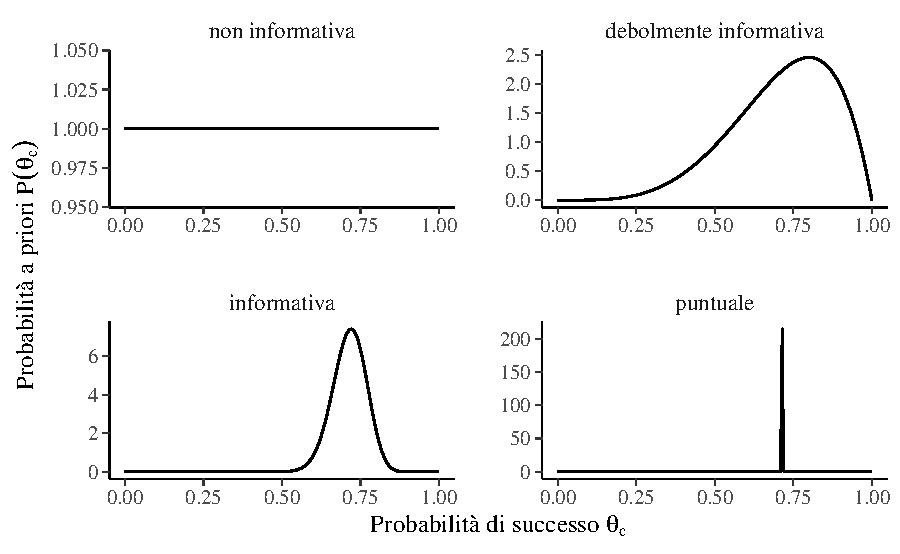
\includegraphics[width=1\linewidth]{ds4psy_files/figure-latex/unnamed-chunk-19-1} 

}

\caption{Uno spinner che riposa a 36 gradi, o il dieci percento del percorso intorno al cerchio. La pendenza dello spinner può assumere qualunque valore tra 0 e 360 gradi.}\label{fig:unnamed-chunk-19}
\end{figure}

Cosa implica per \(\Theta\) dire che lo spinner è simmetrico? Possiamo dire che, in ciascuna prova, la rotazione dello spinner produce un angolo qualunque da 0 a 360 gradi. In altri termini, un valore \(\Theta\) compreso tra 0 e 36 gradi ha la stessa probabilità di essere osservato di un valore \(\Theta\) compreso tra 200 e 236 gradi. Inoltre, poiché 36 gradi è un decimo del percorso intorno al cerchio, la probabilità di ottenere un qualsiasi intervallo di 36 gradi sarà sempre uguale al 10\%. Ovvero \(\mbox{P}[0 \leq \Theta \leq 36] \ = \ \frac{1}{10}\) e \(\mbox{P}[200 \leq \Theta \leq 236] \ = \ \frac{1}{10}\).

È importante notare che le considerazioni precedenti non si riferiscono al fatto che \(\Theta\) può assumere uno specifico valore, ma piuttosto alla probabilità di osservare \(\Theta\) in un particolare intervallo di valori. In generale, la probabilità che la pendenza \(\Theta\) dello spinner cada in intervallo è la frazione del cerchio rappresentata dall'intervallo, cioè,

\[
\mbox{P}[\theta_1 \leq \Theta \leq \theta_2] = \frac{\theta_2 - \theta_1}{360}, \qquad 0 \leq \theta_1 \leq \theta_2 \leq 360.
\]

La ragione di questo è che le variabili casuali continue non hanno una massa di probabilità. Invece, una massa di probabilità viene assegnata alla realizzazione della variabile casuale in un intervallo di valori.

\hypertarget{il-paradosso-delle-variabili-casuali-continue}{%
\subsection{Il paradosso delle variabili casuali continue}\label{il-paradosso-delle-variabili-casuali-continue}}

Nel nostro esempio, la pendenza dello spinner è esattamente 36 gradi; ma avrebbe potuto anche essere 36.0376531 gradi o qualunque altro valore in quell'intorno. Qual è la probabilità che la pendenza dello spinner sia esattamente 36? Paradossalmente, la risposta è zero:

\[
\mbox{P}[\Theta = 36] = 0.
\]

Infatti, se la probabilità di un qualunque valore fosse maggiore di zero, ogni altro possibile valore dovrebbe avere la stessa probabilità, dato che abbiamo assumiamo che tutti i valori \(\Theta\) sono egualmente probabili. Ma se poi andiamo a sommare tutte queste probabilità il totale diventerà maggiore di uno, il che non è possibile.

Nel caso delle variabili casuali continue dobbiamo dunque rinunciare a qualcosa, e quel qualcosa è l'idea che, in una distribuzione continua, ciascun valore puntuale della variabile casuale possa avere una massa di probabilità maggiore di zero. Il paradosso sorge perché una realizzazione della variabile casuale conrtinua produce sempre un qualche numero, ma ciscuno di tali numeri ha probabilità nulla.

\hypertarget{la-funzione-di-ripartizione-per-una-variabile-casuale-continua}{%
\section{La funzione di ripartizione per una variabile casuale continua}\label{la-funzione-di-ripartizione-per-una-variabile-casuale-continua}}

Supponiamo che \(\Theta \sim \mbox{uniform}(0, 360)\) sia la pendenza dello spinner. La funzione di ripartizione (ovvero, la distribuzione cumulativa) è definita esattamente come nel caso delle variabili casuali discrete:

\[
F_{\Theta}(\theta) = \mbox{P}[\Theta \leq \theta].
\]

Cioè, è la probabilità che la variabile casuale \(\Theta\) assuma un valore minore di o uguale a \(\theta\). In questo caso, poiché si presume che lo spinner sia simmetrico, la funzione di distribuzione cumulativa è

\[
F_{\Theta}(\theta) = \frac{\theta}{360}.
\]

Questa è una funzione lineare di \(\theta\), cioè \(\frac{1}{360} \times \theta\), come indicato dal grafico della figura \ref{fig:spinner-cdf}.

\begin{figure}

{\centering 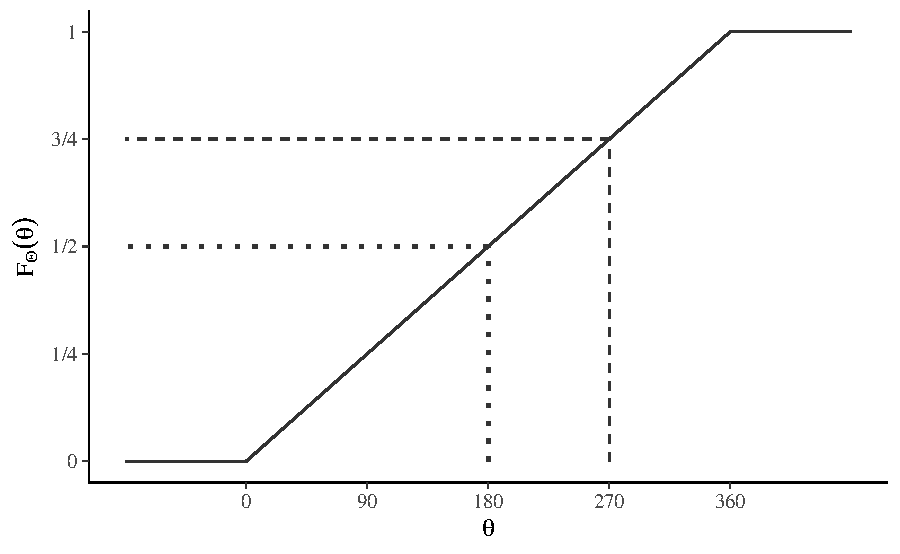
\includegraphics{ds4psy_files/figure-latex/spinner-cdf-1} 

}

\caption{Funzione di distribuzione cumulativa per l'angolo $\theta$ (in gradi) risultante da una rotazione di uno spinner simmetrico. La linea tratteggiata mostra il valore a 180 gradi, che corrisponde ad una probabilità di 0.5, e la linea tratteggiata a 270 gradi, che corrisponde ad una probabilità di 0.75.}\label{fig:spinner-cdf}
\end{figure}

Possiamo verificare questo risultato mediante simulazione. Per stimare la funzione di ripartizione, simuliamo \(M\) valori \(\theta^{(m)}\) e poi li ordiniamo in ordine crescente.

\begin{Shaded}
\begin{Highlighting}[]
\NormalTok{M }\OtherTok{\textless{}{-}} \DecValTok{1000}
\NormalTok{theta }\OtherTok{\textless{}{-}} \FunctionTok{runif}\NormalTok{(M, }\DecValTok{0}\NormalTok{, }\DecValTok{360}\NormalTok{)}
\NormalTok{theta\_asc }\OtherTok{\textless{}{-}} \FunctionTok{sort}\NormalTok{(theta)}
\NormalTok{prob }\OtherTok{\textless{}{-}}\NormalTok{ (}\DecValTok{1}\SpecialCharTok{:}\NormalTok{M) }\SpecialCharTok{/}\NormalTok{ M}
\NormalTok{unif\_cdf\_df }\OtherTok{\textless{}{-}} \FunctionTok{data.frame}\NormalTok{(}
  \AttributeTok{theta =}\NormalTok{ theta\_asc,}
  \AttributeTok{prob =}\NormalTok{ prob}
\NormalTok{)}
\NormalTok{unif\_cdf\_plot }\OtherTok{\textless{}{-}}
\NormalTok{  unif\_cdf\_df }\SpecialCharTok{\%\textgreater{}\%}
  \FunctionTok{ggplot}\NormalTok{(}\FunctionTok{aes}\NormalTok{(}\AttributeTok{x =}\NormalTok{ theta, }\AttributeTok{y =}\NormalTok{ prob)) }\SpecialCharTok{+}
  \FunctionTok{geom\_line}\NormalTok{() }\SpecialCharTok{+}
  \FunctionTok{scale\_x\_continuous}\NormalTok{(}\AttributeTok{breaks =} \FunctionTok{c}\NormalTok{(}\DecValTok{0}\NormalTok{, }\DecValTok{90}\NormalTok{, }\DecValTok{180}\NormalTok{, }\DecValTok{270}\NormalTok{, }\DecValTok{360}\NormalTok{)) }\SpecialCharTok{+}
  \FunctionTok{scale\_y\_continuous}\NormalTok{(}\AttributeTok{breaks =} \FunctionTok{c}\NormalTok{(}\DecValTok{0}\NormalTok{, }\FloatTok{0.25}\NormalTok{, }\FloatTok{0.5}\NormalTok{, }\FloatTok{0.75}\NormalTok{, }\FloatTok{1.0}\NormalTok{)) }\SpecialCharTok{+}
  \FunctionTok{xlab}\NormalTok{(}\FunctionTok{expression}\NormalTok{(theta)) }\SpecialCharTok{+}
  \FunctionTok{ylab}\NormalTok{(}\FunctionTok{expression}\NormalTok{(F[Theta](theta)))}
\NormalTok{unif\_cdf\_plot}
\end{Highlighting}
\end{Shaded}

\begin{figure}

{\centering 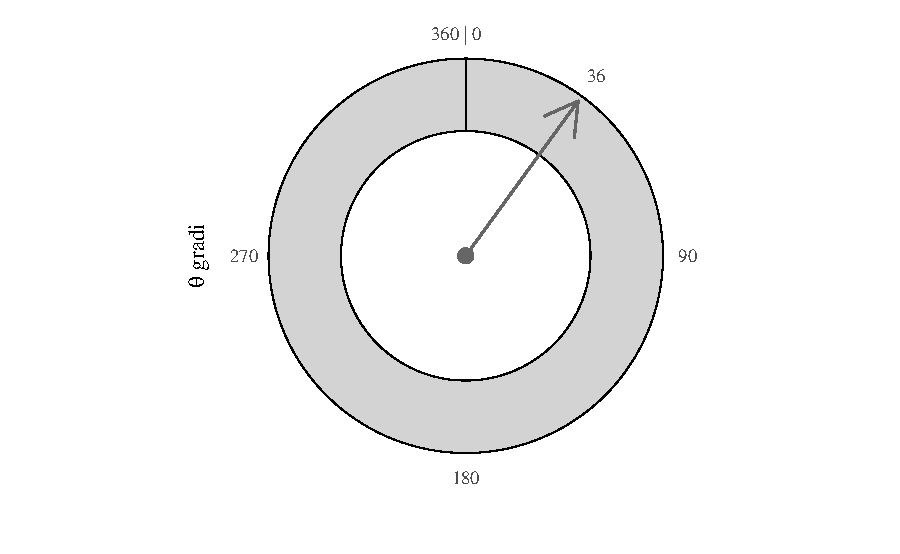
\includegraphics{ds4psy_files/figure-latex/unnamed-chunk-20-1} 

}

\caption{Grafico della funzione di ripartizione di una variabile casuale $\Theta$ che rappresenta il risultato di una rotazione di uno spinner simmetrico. Come previsto, tale funzione è una semplice funzione lineare perché la variabile sottostante $\Theta$ ha una distribuzione uniforme.}\label{fig:unnamed-chunk-20}
\end{figure}

Anche con \emph{M} = 1000, tale grafico è praticamente indistinguibile da quello prodotto per via analitica.

Come nel caso delle variabili casuali discrete, la funzione di ripartizione può essere utilizzata per calcolare le probabilità che la variabile casuale assuma valori in un intervallo. Ad esempio

\begin{align}
\mbox{P}[180 < \Theta \leq 270] &= \mbox{P}[\Theta \leq 270] \ - \ \mbox{P}[\Theta \leq 180] \notag\\
&= F_{\Theta}(270) - F_{\Theta}(180)\notag\\
&= \frac{3}{4} - \frac{1}{2} \notag\\
&= \frac{1}{4}.\noindent
\end{align}

\hypertarget{la-distribuzione-uniforme}{%
\section{La distribuzione uniforme}\label{la-distribuzione-uniforme}}

Dopo avere visto come generare numeri casuali uniformi da 0 a 360, consideriamo ora una variabile casuale che assume valori nell'intervallo da 0 a 1. Chiamiamo tale variabile casuale \(\Theta\) e assumiamo che abbia una distribuzione continua uniforme sull'intervallo {[}0, 1{]}:

\[
\Theta \sim Uniform(0, 1).
\]

Poiché le probabilità assumono valori nell'intervallo {[}0, 1{]}, possiamo pensare a \(\Theta\) come ad un valore di probabilità preso a caso in ciascuna realizzazione dell'esperimento casuale.

La distribuzione uniforme è la più semplice delle distribuzioni di densità di probabilità. Per chiarire le proprietà di tale distribuzione, iniziamo con una simulazione e generiamo 10,000 valori casuali di \(\Theta\). I primi 10 di tali valori sono stampati qui di seguito:

\begin{Shaded}
\begin{Highlighting}[]
\FunctionTok{set.seed}\NormalTok{(}\DecValTok{1234}\NormalTok{)}
\NormalTok{M }\OtherTok{\textless{}{-}} \DecValTok{10000}
\NormalTok{logit }\OtherTok{\textless{}{-}} \ControlFlowTok{function}\NormalTok{(x) }\FunctionTok{log}\NormalTok{(x }\SpecialCharTok{/}\NormalTok{ (}\DecValTok{1} \SpecialCharTok{{-}}\NormalTok{ x))}
\NormalTok{theta }\OtherTok{\textless{}{-}} \FunctionTok{runif}\NormalTok{(M)}
\NormalTok{alpha }\OtherTok{\textless{}{-}} \FunctionTok{logit}\NormalTok{(theta)}
\ControlFlowTok{for}\NormalTok{ (m }\ControlFlowTok{in} \DecValTok{1}\SpecialCharTok{:}\DecValTok{10}\NormalTok{) \{}
  \FunctionTok{print}\NormalTok{(alpha[m])}
\NormalTok{\}}
\CommentTok{\#\textgreater{} [1] {-}2.053}
\CommentTok{\#\textgreater{} [1] 0.4993}
\CommentTok{\#\textgreater{} [1] 0.4443}
\CommentTok{\#\textgreater{} [1] 0.5039}
\CommentTok{\#\textgreater{} [1] 1.823}
\CommentTok{\#\textgreater{} [1] 0.5767}
\CommentTok{\#\textgreater{} [1] {-}4.647}
\CommentTok{\#\textgreater{} [1] {-}1.194}
\CommentTok{\#\textgreater{} [1] 0.6905}
\CommentTok{\#\textgreater{} [1] 0.05702}
\end{Highlighting}
\end{Shaded}

Creaiamo ora un istogramma che descrive la distribuzione delle 10,000 realizzazioni \(\Theta\) che abbiamo trovato:

\begin{Shaded}
\begin{Highlighting}[]
\NormalTok{df\_prob\_unif }\OtherTok{\textless{}{-}} \FunctionTok{data.frame}\NormalTok{(}\AttributeTok{theta =}\NormalTok{ theta)}
\NormalTok{unif\_prob\_plot }\OtherTok{\textless{}{-}}
  \FunctionTok{ggplot}\NormalTok{(df\_prob\_unif, }\FunctionTok{aes}\NormalTok{(theta)) }\SpecialCharTok{+}
  \FunctionTok{geom\_histogram}\NormalTok{(}
    \AttributeTok{binwidth =} \DecValTok{1} \SpecialCharTok{/} \DecValTok{34}\NormalTok{, }\AttributeTok{center =} \DecValTok{1} \SpecialCharTok{/} \DecValTok{68}\NormalTok{, }\AttributeTok{color =} \StringTok{"black"}\NormalTok{,}
    \AttributeTok{size =} \FloatTok{0.25}
\NormalTok{  ) }\SpecialCharTok{+}
  \FunctionTok{scale\_x\_continuous}\NormalTok{(}\AttributeTok{breaks =} \FunctionTok{c}\NormalTok{(}\DecValTok{0}\NormalTok{, }\FloatTok{0.25}\NormalTok{, }\FloatTok{0.5}\NormalTok{, }\FloatTok{0.75}\NormalTok{, }\DecValTok{1}\NormalTok{)) }\SpecialCharTok{+}
  \FunctionTok{scale\_y\_continuous}\NormalTok{(}\AttributeTok{lim =} \FunctionTok{c}\NormalTok{(}\DecValTok{0}\NormalTok{, }\DecValTok{1300}\NormalTok{), }\AttributeTok{breaks =} \FunctionTok{c}\NormalTok{(}\DecValTok{500}\NormalTok{, }\DecValTok{1000}\NormalTok{)) }\SpecialCharTok{+}
  \FunctionTok{xlab}\NormalTok{(}\FunctionTok{expression}\NormalTok{(}\FunctionTok{paste}\NormalTok{(Theta, }\StringTok{" \textasciitilde{} Uniform(0, 1)"}\NormalTok{)))}
\NormalTok{unif\_prob\_plot}
\end{Highlighting}
\end{Shaded}

\begin{figure}

{\centering 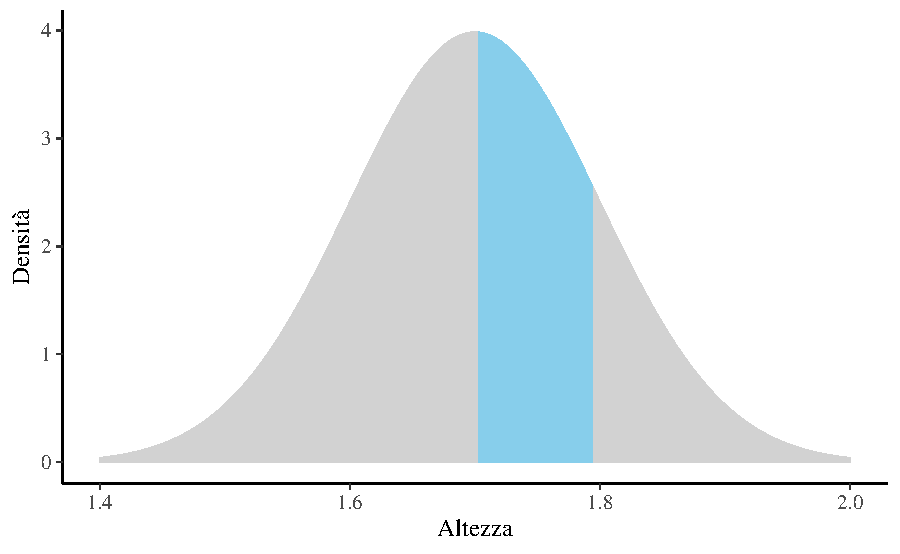
\includegraphics{ds4psy_files/figure-latex/unnamed-chunk-22-1} 

}

\caption{Istogramma di $10\,000$ realizzazioni $\Theta \sim \mbox{Uniform}(0, 1)$. }\label{fig:unnamed-chunk-22}
\end{figure}

È chiaro che, all'aumentare del numero delle realizzazioni \(\Theta\), il profilo dell'istogramma tenderà a diventare una linea retta. Ciò significa che la funzione di densità di una variabile casuale uniforme continua è una costante. Cioè, se \(\Theta \sim \mbox{Uniform} (a, b)\), allora \(p_{\Theta}(\theta) = c\), dove \(c\) è una costante.

\begin{Shaded}
\begin{Highlighting}[]
\NormalTok{uniform\_pdf\_df }\OtherTok{\textless{}{-}} \FunctionTok{data.frame}\NormalTok{(}\AttributeTok{y =} \FunctionTok{c}\NormalTok{(}\DecValTok{0}\NormalTok{, }\DecValTok{1}\NormalTok{), }\AttributeTok{p\_y =} \FunctionTok{c}\NormalTok{(}\DecValTok{1}\NormalTok{, }\DecValTok{1}\NormalTok{))}
\NormalTok{uniform\_pdf\_plot }\OtherTok{\textless{}{-}}
  \FunctionTok{ggplot}\NormalTok{(uniform\_pdf\_df, }\FunctionTok{aes}\NormalTok{(}\AttributeTok{x =}\NormalTok{ y, }\AttributeTok{y =}\NormalTok{ p\_y)) }\SpecialCharTok{+}
  \FunctionTok{geom\_line}\NormalTok{(}\AttributeTok{size =} \FloatTok{0.5}\NormalTok{, }\AttributeTok{color =} \StringTok{"\#333333"}\NormalTok{) }\SpecialCharTok{+}
  \FunctionTok{geom\_point}\NormalTok{(}\AttributeTok{size =} \FloatTok{1.5}\NormalTok{, }\AttributeTok{color =} \StringTok{"\#333333"}\NormalTok{) }\SpecialCharTok{+}
  \FunctionTok{scale\_x\_continuous}\NormalTok{(}\AttributeTok{breaks =} \FunctionTok{c}\NormalTok{(}\DecValTok{0}\NormalTok{, }\DecValTok{1}\NormalTok{), }\AttributeTok{labels =} \FunctionTok{c}\NormalTok{(}\StringTok{"a"}\NormalTok{, }\StringTok{"b"}\NormalTok{)) }\SpecialCharTok{+}
  \FunctionTok{scale\_y\_continuous}\NormalTok{(}
    \AttributeTok{lim =} \FunctionTok{c}\NormalTok{(}\DecValTok{0}\NormalTok{, }\DecValTok{1}\NormalTok{), }\AttributeTok{breaks =} \FunctionTok{c}\NormalTok{(}\DecValTok{0}\NormalTok{, }\DecValTok{1}\NormalTok{),}
    \AttributeTok{labels =} \FunctionTok{c}\NormalTok{(}\StringTok{"0"}\NormalTok{, }\StringTok{"c"}\NormalTok{)}
\NormalTok{  ) }\SpecialCharTok{+}
  \FunctionTok{xlab}\NormalTok{(}\FunctionTok{expression}\NormalTok{(theta)) }\SpecialCharTok{+}
  \FunctionTok{ylab}\NormalTok{(}\FunctionTok{expression}\NormalTok{(}\FunctionTok{paste}\NormalTok{(p[Theta], }\StringTok{"("}\NormalTok{, theta, }\StringTok{" | a, b)"}\NormalTok{))) }\SpecialCharTok{+}
  \FunctionTok{geom\_segment}\NormalTok{(}\FunctionTok{aes}\NormalTok{(}\AttributeTok{x =} \DecValTok{0}\NormalTok{, }\AttributeTok{y =} \DecValTok{0}\NormalTok{, }\AttributeTok{xend =} \DecValTok{0}\NormalTok{, }\AttributeTok{yend =} \DecValTok{1}\NormalTok{),}
    \AttributeTok{linetype =} \StringTok{"dotted"}
\NormalTok{  ) }\SpecialCharTok{+}
  \FunctionTok{geom\_segment}\NormalTok{(}\FunctionTok{aes}\NormalTok{(}\AttributeTok{x =} \DecValTok{1}\NormalTok{, }\AttributeTok{y =} \DecValTok{0}\NormalTok{, }\AttributeTok{xend =} \DecValTok{1}\NormalTok{, }\AttributeTok{yend =} \DecValTok{1}\NormalTok{),}
    \AttributeTok{linetype =} \StringTok{"dotted"}
\NormalTok{  ) }\SpecialCharTok{+}
  \FunctionTok{geom\_segment}\NormalTok{(}\FunctionTok{aes}\NormalTok{(}\AttributeTok{x =} \DecValTok{0}\NormalTok{, }\AttributeTok{y =} \DecValTok{0}\NormalTok{, }\AttributeTok{xend =} \DecValTok{1}\NormalTok{, }\AttributeTok{yend =} \DecValTok{0}\NormalTok{),}
    \AttributeTok{linetype =} \StringTok{"dotted"}
\NormalTok{  ) }\SpecialCharTok{+}
  \FunctionTok{geom\_segment}\NormalTok{(}\FunctionTok{aes}\NormalTok{(}\AttributeTok{x =} \SpecialCharTok{{-}}\FloatTok{0.25}\NormalTok{, }\AttributeTok{y =} \DecValTok{0}\NormalTok{, }\AttributeTok{xend =} \DecValTok{0}\NormalTok{, }\AttributeTok{yend =} \DecValTok{0}\NormalTok{)) }\SpecialCharTok{+}
  \FunctionTok{geom\_segment}\NormalTok{(}\FunctionTok{aes}\NormalTok{(}\AttributeTok{x =} \DecValTok{1}\NormalTok{, }\AttributeTok{y =} \DecValTok{0}\NormalTok{, }\AttributeTok{xend =} \FloatTok{1.25}\NormalTok{, }\AttributeTok{yend =} \DecValTok{0}\NormalTok{)) }\SpecialCharTok{+}
  \FunctionTok{geom\_point}\NormalTok{(}\FunctionTok{aes}\NormalTok{(}\AttributeTok{x =} \DecValTok{0}\NormalTok{, }\AttributeTok{y =} \DecValTok{0}\NormalTok{),}
    \AttributeTok{size =} \FloatTok{1.5}\NormalTok{, }\AttributeTok{shape =} \DecValTok{21}\NormalTok{,}
    \AttributeTok{fill =} \StringTok{"\#ffffe6"}
\NormalTok{  ) }\SpecialCharTok{+}
  \FunctionTok{geom\_point}\NormalTok{(}\FunctionTok{aes}\NormalTok{(}\AttributeTok{x =} \DecValTok{1}\NormalTok{, }\AttributeTok{y =} \DecValTok{0}\NormalTok{),}
    \AttributeTok{size =} \FloatTok{1.5}\NormalTok{, }\AttributeTok{shape =} \DecValTok{21}\NormalTok{,}
    \AttributeTok{fill =} \StringTok{"\#ffffe6"}
\NormalTok{  )}
\NormalTok{uniform\_pdf\_plot}
\end{Highlighting}
\end{Shaded}

\begin{center}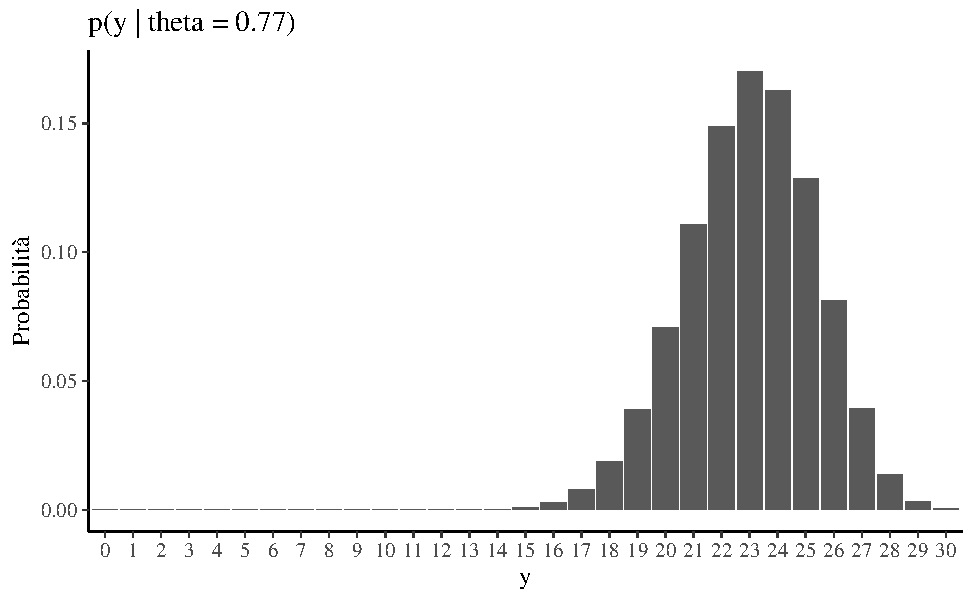
\includegraphics{ds4psy_files/figure-latex/unnamed-chunk-23-1} \end{center}

\noindent Dal grafico vediamo che l'area sottesa alla funzione di densità è \((b - a)\times c\). Dato che tale area deve essere unitaria, ovvero, \((b - a) \times c = 1\), possiamo trovare \(c\) dividendo entrambi i termini per \(b - a\),

\[
c  = \frac{\displaystyle{1}}{\displaystyle b - a}.
\]

Ovvero, se \(\Theta \sim \mbox{Uniform}(a, b)\), allora

\[
p_{\Theta}(\theta) = \mbox{Uniform}(\theta \mid a, b),
\]

laddove

\[
\mbox{Uniform}(\theta \mid a, b) = \frac{1}{b - a}.
\]

In conclusione, la densità di una variabile casuale uniforme continua non dipende da \(\theta\) --- è costante e identica per ogni possibile valore \(\theta\).\footnote{Per comodità, possiamo assumere che i valori impossibili di \(\theta\) abbiano una densità uguale a zero.} Vedremo nel prossimo Paragrafo che, eseguendo una trasformazione su questa variabile casuale uniforme, possiamo creare altre variabili casuali di interesse.

\begin{exercise}
Si consideri una variabile casuale uniforme \(X\) definita sull'intervallo {[}0, 100{]}. Si trovi la probabilità \(P(20 < X < 60)\).

Per trovare la soluzione è sufficiente calcolare l'area di un rettangolo di base \(60 - 20 = 40\) e di altezza 1/100. La probabilità cercata è dunque \(P(20 < X < 60) = 40 \cdot 0.01 = 0.4\).
\end{exercise}

\hypertarget{dagli-istogrammi-alle-densituxe0}{%
\section{Dagli istogrammi alle densità}\label{dagli-istogrammi-alle-densituxe0}}

Non esiste l'equivalente di una funzione di massa di probabilità per le variabili casuali continue. Esiste invece una \emph{funzione di densità di probabilità} la quale, nei termini di una simulazione, può essere concepita nel modo seguente: avendo a disposizione un numero enorme di casi, quando l'intervallo \(\Delta\) di ciascuna classe \(\rightarrow\) 0, la spezzata tende a diventare una curva continua. Tale curva continua \(f(x)\) è detta funzione di densità di probabilità.

Come si trasformano gli istogrammi all'aumentare del numero di osservazioni? Nei grafici seguenti, la numerosità cresce da \(10\) a \(1\,000\,000\).

\begin{Shaded}
\begin{Highlighting}[]
\NormalTok{df\_log\_odds\_growth }\OtherTok{\textless{}{-}} \FunctionTok{data.frame}\NormalTok{()}
\ControlFlowTok{for}\NormalTok{ (log10M }\ControlFlowTok{in} \DecValTok{1}\SpecialCharTok{:}\DecValTok{6}\NormalTok{) \{}
\NormalTok{  M }\OtherTok{\textless{}{-}} \DecValTok{10}\SpecialCharTok{\^{}}\NormalTok{log10M}
\NormalTok{  alpha }\OtherTok{\textless{}{-}} \FunctionTok{logit}\NormalTok{(}\FunctionTok{runif}\NormalTok{(M))}
\NormalTok{  df\_log\_odds\_growth }\OtherTok{\textless{}{-}} \FunctionTok{rbind}\NormalTok{(}
\NormalTok{    df\_log\_odds\_growth,}
    \FunctionTok{data.frame}\NormalTok{(}
      \AttributeTok{alpha =}\NormalTok{ alpha,}
      \AttributeTok{M =} \FunctionTok{rep}\NormalTok{(}\FunctionTok{sprintf}\NormalTok{(}\StringTok{"M = \%d"}\NormalTok{, M), M)}
\NormalTok{    )}
\NormalTok{  )}
\NormalTok{\}}
\NormalTok{log\_odds\_growth\_plot }\OtherTok{\textless{}{-}}
\NormalTok{  df\_log\_odds\_growth }\SpecialCharTok{\%\textgreater{}\%}
  \FunctionTok{ggplot}\NormalTok{(}\FunctionTok{aes}\NormalTok{(alpha)) }\SpecialCharTok{+}
  \FunctionTok{geom\_histogram}\NormalTok{(}\AttributeTok{color =} \StringTok{"black"}\NormalTok{, }\AttributeTok{bins =} \DecValTok{75}\NormalTok{) }\SpecialCharTok{+}
  \FunctionTok{facet\_wrap}\NormalTok{(}\SpecialCharTok{\textasciitilde{}}\NormalTok{M, }\AttributeTok{scales =} \StringTok{"free"}\NormalTok{) }\SpecialCharTok{+}
  \FunctionTok{scale\_x\_continuous}\NormalTok{(}
    \AttributeTok{lim =} \FunctionTok{c}\NormalTok{(}\SpecialCharTok{{-}}\FloatTok{8.5}\NormalTok{, }\FloatTok{8.5}\NormalTok{), }\AttributeTok{breaks =} \FunctionTok{c}\NormalTok{(}\SpecialCharTok{{-}}\DecValTok{5}\NormalTok{, }\DecValTok{0}\NormalTok{, }\DecValTok{5}\NormalTok{)}
\NormalTok{  ) }\SpecialCharTok{+}
  \FunctionTok{xlab}\NormalTok{(}\FunctionTok{expression}\NormalTok{(}\FunctionTok{paste}\NormalTok{(Phi, }\StringTok{" = "}\NormalTok{, }\FunctionTok{logit}\NormalTok{(Theta)))) }\SpecialCharTok{+}
  \FunctionTok{ylab}\NormalTok{(}\StringTok{"proportion of draws"}\NormalTok{) }\SpecialCharTok{+}
  \FunctionTok{theme}\NormalTok{(}
    \AttributeTok{axis.text.y =} \FunctionTok{element\_blank}\NormalTok{(),}
    \AttributeTok{axis.ticks.y =} \FunctionTok{element\_blank}\NormalTok{(),}
    \AttributeTok{panel.spacing.x =} \FunctionTok{unit}\NormalTok{(}\DecValTok{2}\NormalTok{, }\StringTok{"lines"}\NormalTok{),}
    \AttributeTok{panel.spacing.y =} \FunctionTok{unit}\NormalTok{(}\DecValTok{2}\NormalTok{, }\StringTok{"lines"}\NormalTok{)}
\NormalTok{  )}
\NormalTok{log\_odds\_growth\_plot}
\end{Highlighting}
\end{Shaded}

\begin{figure}

{\centering 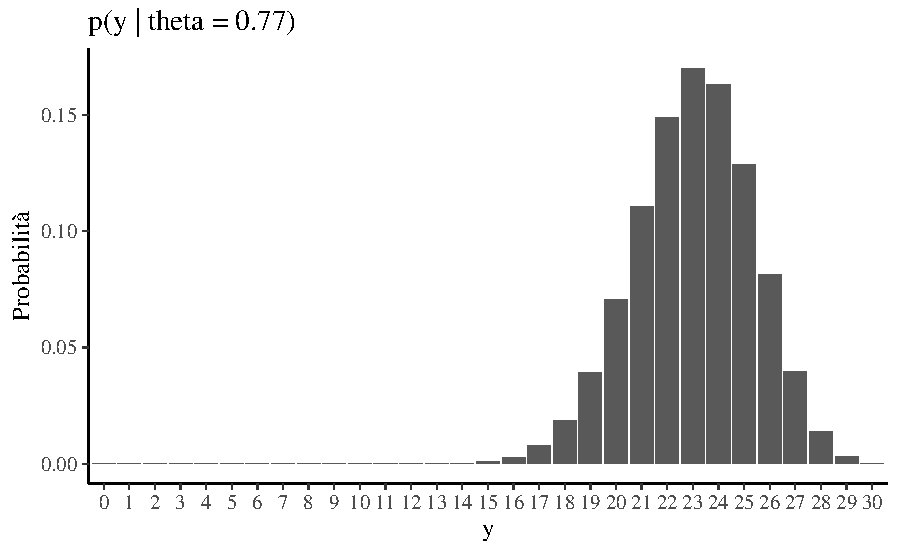
\includegraphics[width=1\linewidth]{ds4psy_files/figure-latex/unnamed-chunk-24-1} 

}

\caption{Istogramma di $M$ campioni casuali $\Theta \sim \mbox{Uniform}(0, 1)$ trasformati in valori $\Phi = \mbox{logit}(\Theta).$ Il profilo limite dell'istogramma è evidenziato nella figura in basso a destra che è stata costruita usando $1\,000\,000$ di osservazioni.}\label{fig:unnamed-chunk-24}
\end{figure}

In un istogramma, l'area di ciascuna barra è proporzionale alla frequenza relativa delle osservazioni in quel'intervallo. Perché tutti gli intervalli hanno la stessa ampiezza, anche l'altezza di ciascuna barra sarà proporzionale alla frequenza relativa delle osservazioni in quel'intervallo.

Nella simulazione, possiamo pensare all'area di ciascuna barra dell'istogramma come alla stima della probabilità che la variabile casuale assuma un valore compreso nell'intervallo considerato. All'aumentare del numero \(M\) di osservazioni, le probabilità stimate si avvicinano sempre di più ai veri valori della probabilità. All'aumentare del numero degli intervalli (quando l'ampiezza \(\Delta\) dell'intervallo \(\rightarrow\) 0), il profilo dell'istogramma tende a diventare una curva continua. Tale curva continua è la funzione di densità di probabilità della variabile casuale. Per l'esempio presente, con \(M =1\,000\,000\), otteniamo il grafico riportato nella figura \ref{fig:hist-dens-example}.

\begin{Shaded}
\begin{Highlighting}[]
\NormalTok{M }\OtherTok{\textless{}{-}} \FloatTok{1e6}
\NormalTok{alpha }\OtherTok{\textless{}{-}} \FunctionTok{logit}\NormalTok{(}\FunctionTok{runif}\NormalTok{(M))}
\NormalTok{density\_limit\_df }\OtherTok{\textless{}{-}} \FunctionTok{data.frame}\NormalTok{(}\AttributeTok{alpha =}\NormalTok{ alpha)}
\NormalTok{density\_limit\_plot }\OtherTok{\textless{}{-}}
\NormalTok{  density\_limit\_df }\SpecialCharTok{\%\textgreater{}\%}
  \FunctionTok{ggplot}\NormalTok{(}\FunctionTok{aes}\NormalTok{(alpha)) }\SpecialCharTok{+}
  \FunctionTok{geom\_histogram}\NormalTok{(}
    \AttributeTok{stat =} \StringTok{"density"}\NormalTok{, }\AttributeTok{n =} \DecValTok{75}\NormalTok{, }\AttributeTok{color =} \StringTok{"black"}\NormalTok{, }\AttributeTok{size =} \FloatTok{0.15}
\NormalTok{  ) }\SpecialCharTok{+}
  \FunctionTok{stat\_function}\NormalTok{(}
    \AttributeTok{fun =}\NormalTok{ dlogis,}
    \AttributeTok{args =} \FunctionTok{list}\NormalTok{(}\AttributeTok{location =} \DecValTok{0}\NormalTok{, }\AttributeTok{scale =} \DecValTok{1}\NormalTok{),}
    \AttributeTok{col =} \StringTok{"black"}\NormalTok{,}
    \AttributeTok{size =} \FloatTok{0.3}
\NormalTok{  ) }\SpecialCharTok{+}
  \FunctionTok{scale\_x\_continuous}\NormalTok{(}
    \AttributeTok{lim =} \FunctionTok{c}\NormalTok{(}\SpecialCharTok{{-}}\DecValTok{9}\NormalTok{, }\DecValTok{9}\NormalTok{),}
    \AttributeTok{breaks =} \FunctionTok{c}\NormalTok{(}\SpecialCharTok{{-}}\DecValTok{6}\NormalTok{, }\SpecialCharTok{{-}}\DecValTok{4}\NormalTok{, }\SpecialCharTok{{-}}\DecValTok{2}\NormalTok{, }\DecValTok{0}\NormalTok{, }\DecValTok{2}\NormalTok{, }\DecValTok{4}\NormalTok{, }\DecValTok{6}\NormalTok{)}
\NormalTok{  ) }\SpecialCharTok{+}
  \FunctionTok{xlab}\NormalTok{(}
    \FunctionTok{expression}\NormalTok{(}\FunctionTok{paste}\NormalTok{(Phi, }\StringTok{" = "}\NormalTok{, }\FunctionTok{logit}\NormalTok{(Theta)))}
\NormalTok{  ) }\SpecialCharTok{+}
  \FunctionTok{ylab}\NormalTok{(}\StringTok{"Frequenza relativa"}\NormalTok{) }\SpecialCharTok{+}
  \FunctionTok{theme}\NormalTok{(}
    \AttributeTok{axis.text.y =} \FunctionTok{element\_blank}\NormalTok{(),}
    \AttributeTok{axis.ticks.y =} \FunctionTok{element\_blank}\NormalTok{()}
\NormalTok{  )}
\NormalTok{density\_limit\_plot}
\end{Highlighting}
\end{Shaded}

\begin{figure}

{\centering 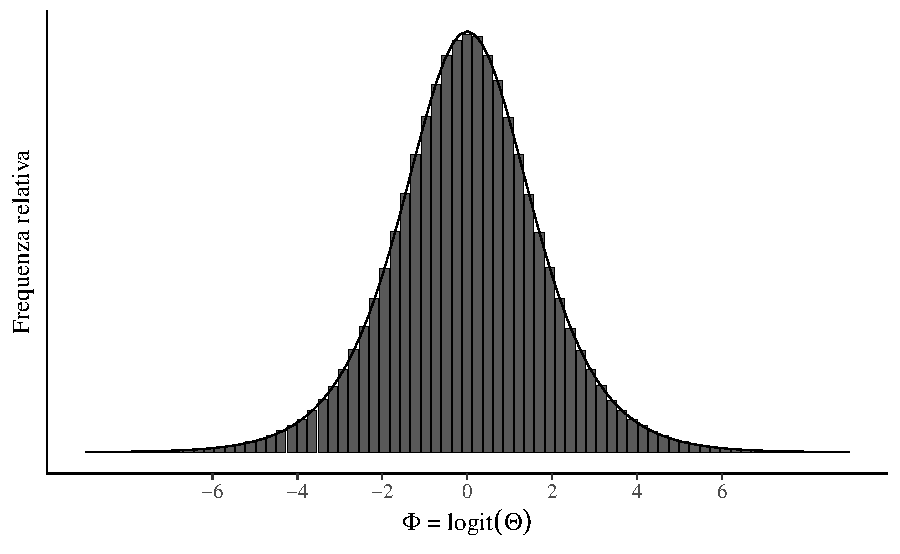
\includegraphics[width=1\linewidth]{ds4psy_files/figure-latex/hist-dens-example-1} 

}

\caption{Istogramma di $M = 1\,000\,000$ campioni casuali $\Theta \sim \mbox{Uniform}(0,1)$ trasformati in valori $\Phi = \mbox{logit}(\Theta)$. La spezzata nera congiunge i punti centrali superiori delle barre dell'istogramma. Nel limite, quando il numero di osservazioni e di barre tende all'infinito, tale spezzata approssima la funzione di densità di probabilità della variabile casuale.}\label{fig:hist-dens-example}
\end{figure}

Nella statistica descrittiva abbiamo già incontrato una rappresentazione che ha lo stesso significato della funzione di densità, ovvero il kernel density plot. La stima della densità del kernel (KDE), infatti, è un modo non parametrico per stimare la funzione di densità di probabilità di una variabile casuale.

\hypertarget{funzione-di-densituxe0-di-probabilituxe0}{%
\section{Funzione di densità di probabilità}\label{funzione-di-densituxe0-di-probabilituxe0}}

Per descrivere le probabilità che possono essere associate ad una variabile casuale continua \(X\) è necessario definire una funzione \(p(X)\) che deve soddisfare le seguenti due proprietà:

\begin{itemize}
\item
  \(p(x) \geq 0, \forall x\), ovvero, l'ordinata della funzione di densità è 0 o positiva;
\item
  \(\int_{-\infty}^{\infty} p(x) \,\operatorname {d}\!x = 1\), ovvero, l'area sottesa dalla \(p(x)\) è unitaria\footnote{Per quel che riguarda la notazione dell'integrale, ovvero \(\int_x \,\operatorname {d}\!x\), rimando alla discussione di S.P. Thompson: \url{https://calculusmadeeasy.org/1.html}};
\item
  \(p(a < x < b) = \int_a^b p(x) \,\operatorname {d}\!x\), se \(a \leq b\), ovvero, l'area sottesa dalla \(p(y)\) tra due punti \(a\) e \(b\) corrisponde alla probabilità che la v.c. \(x\) assuma un valore compresto tra questi due estremi.
\end{itemize}

\emph{Interpretazione.} È possibile che \(p(x) > 1\), quindi una densità di probabilità non può essere interpretata come una probabilità. Piuttosto, la densità \(p(x)\) può essere utilizzata per confrontare la plausibilità relativa di diversi valori \(X\). Considerata una variabile casuale \(X\) di cui è disponibile un insieme di realizzazioni, tanto maggiore è \(p(x_k)\) rispetto a \(p(x_l)\), tanto più grande sarà la nostra certezza che valori nell'intorno di \(x_k\) verranno osservati con maggiore frequenza di valori nell'intorno di \(x_l\).

\hypertarget{la-funzione-di-ripartizione}{%
\section{La funzione di ripartizione}\label{la-funzione-di-ripartizione}}

La funzione di ripartizione \(F(X)\) è quella funzione che associa a ogni valore di una variabile aleatoria \(X\) la probabilità che la variabile assuma valore minore o uguale a un prefissato valore \(x_k\).

La funzione di ripartizione è sempre non negativa, monotona non decrescente tra \(0\) e \(1\), tale che:

\[
\lim_{x \to -\infty} F_x(X) = F_X(-\infty) = 0, \quad \lim_{x \to +\infty} F_X(X) = F_X(+\infty) = 1.
\]

Se \(X\) è una variabile aleatoria discreta, tale funzione può essere espressa nel seguente modo:

\[
F(x_k) = P(X \leq x_k) = \sum_{i=1}^k P(X = x_i),
\]

dove \(P(X = xi)\) rappresenta la probabilità che la variabile aleatoria \(X\) assuma la modalità \(x_i\).

Se \(X\) è una variabile aleatoria continua allora la funzione di ripartizione è:

\[
F(x_k) = P(X \leq x_k) = \int_{-\infty}^{x_k} f(x) \,\operatorname {d}\!x .
\]

\hypertarget{exp-val-and-variance-rv}{%
\chapter{Valore atteso e varianza}\label{exp-val-and-variance-rv}}

Spesso risulta utile fornire una rappresentazione sintetica della distribuzione di una variabile casuale attraverso degli indicatori caratteristici piuttosto che fare riferimento ad una sua rappresentazione completa mediante la funzione di ripartizione, o la funzione di massa o di densità di probabilità. Una descrizione più sintetica di una variabile casuale, tramite pochi valori, ci consente di cogliere le caratteristiche essenziali della distribuzione, quali: la posizione, cioè il baricentro della distribuzione di probabilità; la variabilità, cioè la dispersione della distribuzione di probabilità attorno ad un centro; la forma della distribuzione di probabilità, considerando la simmetria e la curtosi (pesantezza delle code). In questo Capitolo introdurremo quegli indici sintetici che descrivono il centro di una distribuzione di probabilità e la sua variabilità.

\hypertarget{valore-atteso}{%
\section{Valore atteso}\label{valore-atteso}}

Quando vogliamo conoscere il comportamento tipico di una variabile casuale spesso vogliamo sapere qual è il suo ``valore tipico''. La nozione di ``valore tipico'', tuttavia, è ambigua. Infatti, essa può essere definita in almeno tre modi diversi:

\begin{itemize}
\tightlist
\item
  la \emph{media} (somma dei valori divisa per il numero dei valori),
\item
  la \emph{mediana} (il valore centrale della distribuzione, quando la variabile è ordinata in senso crescente o decrescente),
\item
  la \emph{moda} (il valore che ricorre più spesso).
\end{itemize}

Per esempio, la media di \(\{3, 1, 4, 1, 5\}\) è \(\frac{3+1+4+1+5}{5} = 2.8\), la mediana è \(3\) e la moda è \(1\). Tuttavia, la teoria delle probabilità si occupa di variabili casuali piuttosto che di sequenze di numeri. Diventa dunque necessario precisare che cosa intendiamo per ``valore tipico'' quando facciamo riferimento alle variabili casuali. Giungiamo così alla seguente definizione.

\begin{definition}
Sia \(Y\) è una variabile casuale discreta che assume i valori \(y_1, \dots, y_n\) con distribuzione \(p(y)\), ossia

\[
P(Y = y_i) = p(y_i),
\]

per definizione il \emph{valore atteso} di \(Y\), \(\E(Y)\), è

\begin{equation}
\E(Y) = \sum_{i=1}^n y_i \cdot p(y_i).
\label{eq:expval-discr}
\end{equation}
\end{definition}

A parole: il valore atteso (o speranza matematica, o aspettazione, o valor medio) di una variabile casuale è definito come la somma di tutti i valori che la variabile casuale può prendere, ciascuno pesato dalla probabilità con cui il valore è preso.

\begin{exercise}
Calcoliamo il valore atteso della variabile casuale \(Y\) corrispondente al lancio di una moneta equilibrata (testa: \emph{Y} = 1; croce: \emph{Y} = 0).

\[
\E(Y) = \sum_{i=1}^{2} y_i \cdot P(y_i) = 0 \cdot \frac{1}{5} + 1 \cdot \frac{1}{5} = 0.5.
\]
\end{exercise}

\begin{exercise}
Supponiamo ora che \emph{Y} sia il risultato del lancio di un dado equilibrato. Il valore atteso di \emph{Y} diventa:

\[
\E(Y) = \sum_{i=1}^{6} y_i \cdot P(y_i) = 1 \cdot \frac{1}{6} + 2 \cdot \frac{1}{6} + \dots + 6 \cdot \frac{1}{6} = \frac{21}{6} = 3.5.
\]
\end{exercise}

\hypertarget{interpretazione}{%
\subsection{Interpretazione}\label{interpretazione}}

Che interpretazione può essere assegnata alla nozione di valore atteso? Bruno de Finetti adottò lo stesso termine di \emph{previsione} (e lo stesso simbolo) tanto per la probabilità che per la speranza matematica. Si può pertanto dire che, dal punto di vista bayesiano, la speranza matematica è l'estensione naturale della nozione di probabilità soggettiva.

\hypertarget{proprietuxe0-del-valore-atteso}{%
\subsection{Proprietà del valore atteso}\label{proprietuxe0-del-valore-atteso}}

La proprietà più importante del valore atteso è la linearità: il valore atteso di una somma di variabili casuali è uguale alla somma dei lori rispettivi valori attesi:

\begin{equation}
\E(X + Y) = \E(X) + \E(Y).
\label{eq:prop-expval-linearity}
\end{equation}

La \eqref{eq:prop-expval-linearity} sembra ragionevole quando \(X\) e \(Y\) sono indipendenti, ma è anche vera quando \(X\) e \(Y\) sono associati. Abbiamo anche che

\begin{equation}
\E(cY) = c \E(Y).
\label{eq:prop-expval-const}
\end{equation}

La \eqref{eq:prop-expval-const} ci dice che possiamo estrarre una costante dall'operatore di valore atteso. Tale proprietà si estende a qualunque numero di variabili casuali. Infine, se due variabili casuali \(X\) e \(Y\) sono indipendenti, abbiamo che

\begin{equation}
\E(X Y) = \E(X) \E(Y). 
\label{eq:expval-prod-ind-rv}
\end{equation}

\begin{exercise}
Si considerino le seguenti variabili casuali: \(Y\), ovvero il numero che si ottiene dal lancio di un dado equilibrato, e \(Y\), il numero di teste prodotto dal lancio di una moneta equilibrata. Poniamoci il problema di trovare il valore atteso di \(X+Y\).

Per risolvere il problema iniziamo a costruire lo spazio campionario dell'esperimento casuale consistente nel lancio di un dado e di una moneta.

\begin{longtable}[]{@{}ccccccc@{}}
\toprule
\(x/ y\) & 1 & 2 & 3 & 4 & 5 & 6 \\
\midrule
\endhead
0 & (0, 1) & (0, 2) & (0, 3) & (0, 4) & (0, 5) & (0, 6) \\
1 & (1, 1) & (1, 2) & (1, 3) & (1, 4) & (1, 5) & (1, 6) \\
\bottomrule
\end{longtable}

\noindent ovvero

\begin{longtable}[]{@{}ccccccc@{}}
\toprule
\(x/ y\) & 1 & 2 & 3 & 4 & 5 & 6 \\
\midrule
\endhead
0 & 1 & 2 & 3 & 4 & 5 & 6 \\
1 & 2 & 3 & 4 & 5 & 6 & 7 \\
\bottomrule
\end{longtable}

\noindent Il risultato del lancio del dado è indipendente dal risultato del lancio della moneta. Pertanto, ciascun evento elementare dello spazio campionario avrà la stessa probabilità di verificarsi, ovvero \(Pr(\omega) = \frac{1}{12}\). Il valore atteso di \(X+Y\) è dunque uguale a:

\[
\E(X+Y) = 1 \cdot \frac{1}{12} + 2 \cdot \frac{1}{12} + \dots + 7 \cdot \frac{1}{12} = 4.0.
\]

Lo stesso risultato si ottiene nel modo seguente:

\[
\E(X+Y) = \E(X) + E(Y) = 3.5 + 0.5 = 4.0.
\]
\end{exercise}

\begin{exercise}
Si considerino le variabili casuali \(X\) e \(Y\) definite nel caso del lancio di tre monete equilibrate, dove \(X\) conta il numero delle teste nei tre lanci e \(Y\) conta il numero delle teste al primo lancio. Si calcoli il valore atteso del prodotto delle variabili casuali \(X\) e \(Y\).

La distribuzione di probabilità congiunta \(P(X, Y)\) è fornita nella tabella seguente.

\begin{longtable}[]{@{}cccc@{}}
\toprule
\(x/ y\) & 0 & 1 & \(p(Y)\) \\
\midrule
\endhead
0 & 1/8 & 0 & 1/8 \\
1 & 2/8 & 1/8 & 3/8 \\
2 & 1/8 & 2/8 & 3/8 \\
3 & 0 & 1/8 & 1/8 \\
\(p(y)\) & 4/8 & 4/8 & 1.0 \\
\bottomrule
\end{longtable}

\noindent Il calcolo del valore atteso di \(XY\) si riduce a

\[
\E(XY) = 1 \cdot \frac{1}{8} + 2 \cdot \frac{2}{8} + 3 \cdot \frac{1}{8} = 1.0.
\]

Si noti che le variabili casuali \(Y\) e \(Y\) non sono indipendenti. Dunque non possiamo usare la proprietà \ref{thm:prodindrv}. Infatti, il valore atteso di \(X\) è

\[
\E(X) = 1 \cdot \frac{3}{8} + 2 \cdot \frac{3}{8} + 3 \cdot \frac{1}{8} = 1.5
\]

e il valore atteso di \(Y\) è

\[
\E(Y) = 0 \cdot \frac{4}{8} + 1 \cdot \frac{4}{8} = 0.5.
\] Dunque

\[
1.5 \cdot 0.5 \neq 1.0.
\]
\end{exercise}

\hypertarget{variabili-casuali-continue}{%
\subsection{Variabili casuali continue}\label{variabili-casuali-continue}}

Nel caso di una variabile casuale continua \(Y\) il valore atteso diventa:

\begin{equation}
\E(Y) = \int_{-\infty}^{+\infty} y p(y) \,\operatorname {d}\!y
\label{eq:def-ev-rv-cont}
\end{equation}

Anche in questo caso il valore atteso è una media ponderata della \(y\), nella quale ciascun possibile valore \(y\) è ponderato per il corrispondente valore della densità \(p(y)\). Possiamo leggere l'integrale pensando che \(y\) rappresenti l'ampiezza delle barre infinitamente strette di un istogramma, con la densità \(p(y)\) che corrisponde all'altezza di tali barre e la notazione \(\int_{-\infty}^{+\infty}\) che corrisponde ad una somma.

Un'altra misura di tendenza centrale delle variabili casuali continue è la moda. La moda della \(Y\) individua il valore \(y\) più plausibile, ovvero il valore \(y\) che massimizza la funzione di densità \(p(y)\):

\begin{equation}
\Mo(Y) = \argmax_y p(y).
\label{eq:def-mode}
\end{equation}

\hypertarget{varianza}{%
\section{Varianza}\label{varianza}}

La seconda più importante proprietà di una variabile casuale, dopo che conosciamo il suo valore atteso, è la \emph{varianza}.

\begin{definition}
Se \(Y\) è una variabile casuale discreta con distribuzione \(p(y)\), per definizione la varianza di \(Y\), \(\Var(Y)\), è

\begin{equation}
\Var(Y) = \E\Big[\big(Y - \E(Y)\big)^2\Big].
\label{eq:def-var-rv}
\end{equation}
\end{definition}

A parole: la varianza è la deviazione media quadratica della variabile dalla sua media.\footnote{Data una variabile casuale \(Y\) con valore atteso \(\E(Y)\), le ``distanze'' tra i valori di \(Y\) e il valore atteso \(\E(Y)\) definiscono la variabile casuale \(Y - \E(Y)\) chiamata \emph{scarto}, oppure \emph{deviazione} oppure \emph{variabile casuale centrata}. La variabile \(Y - \E(Y)\) equivale ad una traslazione di sistema di riferimento che porta il valore atteso nell'origine degli assi. Si può dimostrare facilmente che il valore atteso della variabile scarto \(Y - \E(Y)\) vale zero, dunque la media di tale variabile non può essere usata per quantificare la ``dispersione'' dei valori di \(Y\) relativamente al suo valore medio. Occorre rendere sempre positivi i valori di \(Y - \E(Y)\) e tale risultato viene ottenuto considerando la variabile casuale \(\left(Y - \E(Y)\right)^2\).} Se denotiamo \(\E(Y) = \mu\), la varianza \(\Var(Y)\) diventa il valore atteso di \((Y - \mu)^2\).

\begin{exercise}
Posta \(S\) uguale alla somma dei punti ottenuti nel lancio di due dadi equilibrati, poniamoci il problema di calcolare la varianza di \(S\).

La variabile casuale \(S\) ha la seguente distribuzione di probabilità:

\begin{longtable}[]{@{}cccccccccccc@{}}
\toprule
\(s\) & 2 & 3 & 4 & 5 & 6 & 7 & 8 & 9 & 10 & 11 & 12 \\
\midrule
\endhead
\(P(S = s)\) & \(\frac{1}{36}\) & \(\frac{2}{36}\) & \(\frac{3}{36}\) & \(\frac{4}{36}\) & \(\frac{5}{36}\) & \(\frac{6}{36}\) & \(\frac{5}{36}\) & \(\frac{4}{36}\) & \(\frac{3}{36}\) & \(\frac{2}{36}\) & \(\frac{1}{36}\) \\
\bottomrule
\end{longtable}

\noindent Essendo \(\E(S) = 7\), la varianza diventa

\begin{align}
\Var(S) &= \sum \left(S- \mathbb{E}(S)\right)^2 \cdot P(S) \notag\\
&= (2 - 7)^2 \cdot 0.0278 + (3-7)^2 \cdot 0.0556 + \dots + (12 - 7)^2 \cdot 0.0278 \notag\\
&= 5.8333.\notag
\end{align}
\end{exercise}

\hypertarget{formula-alternativa-per-la-varianza}{%
\subsection{Formula alternativa per la varianza}\label{formula-alternativa-per-la-varianza}}

C'è un modo più semplice per calcolare la varianza:

\begin{align}
\E\Big[\big(X - \E(Y)\big)^2\Big] &= \E\big(X^2 - 2X\E(Y) + \E(Y)^2\big)\notag\\
&= \E(Y^2) - 2\E(Y)\E(Y) + \E(Y)^2,\notag
\end{align}

dato che \(\E(Y)\) è una costante; pertanto

\begin{equation}
\Var(Y) = \E(Y^2) - \big(\E(Y) \big)^2.
\label{eq:def-alt-var-rv}
\end{equation}

A parole: la varianza è la media dei quadrati meno il quadrato della media.

\begin{exercise}
Consideriamo la variabile casuale \(Y\) che corrisponde al numero di teste che si osservano nel lancio di una moneta truccata con probabilità di testa uguale a 0.8. Il valore atteso di \(Y\) è

\[
\E(Y) = 0 \cdot 0.2 + 1 \cdot 0.8 = 0.8.
\] Usando la formula tradizionale della varianza otteniamo:

\[
\Var(Y) = (0 - 0.8)^2 \cdot 0.2 + (1 - 0.8)^2 \cdot 0.8 = 0.16.
\] Lo stesso risultato si trova con la formula alternativa della varianza. Il valore atteso di \(Y^2\) è

\[
\E(Y^2) = 0^2 \cdot 0.2 + 1^2 * 0.8 = 0.8.
\] e la varianza diventa

\[
\Var(Y) = \E(Y^2) - \big(\E(Y) \big)^2 = 0.8 - 0.8^2 = 0.16.
\]
\end{exercise}

\hypertarget{variabili-casuali-continue-1}{%
\subsection{Variabili casuali continue}\label{variabili-casuali-continue-1}}

Nel caso di una variabile casuale continua \(Y\), la varianza diventa:

\begin{equation}
\Var(Y) = \int_{-\infty}^{+\infty} \large[y - \E(Y)\large]^2 p(y) \,\operatorname {d}\!y
\label{eq:def-var-rv-cont}
\end{equation}

Come nel caso discreto, la varianza di una v.c. continua \(y\) misura approssimativamente la distanza al quadrato tipica o prevista dei possibili valori \(y\) dalla loro media.

\hypertarget{deviazione-standard}{%
\section{Deviazione standard}\label{deviazione-standard}}

Quando lavoriamo con le varianze, i termini sono innalzati al quadrato e quindi i numeri possono diventare molto grandi (o molto piccoli). Per trasformare nuovamente i valori nell'unità di misura della scala originaria si prende la radice quadrata. Il valore risultante viene chiamato \emph{deviazione standard} e solitamente è denotato dalla lettera greca \(\sigma\).

\begin{definition}
Si definisce scarto quadratico medio (o deviazione standard o scarto tipo) la radice quadrata della varianza:

\begin{equation}
\sigma_Y = \sqrt{\Var(Y)}.
\label{eq:def-sd}
\end{equation}
\end{definition}

Interpretiamo la deviazione standard di una variabile casuale come nella statistica descrittiva: misura approssimativamente la distanza tipica o prevista dei possibili valori \(y\) dalla loro media.

\begin{exercise}
Per i dadi equilibrati dell'esempio precedente, la deviazione standard della variabile casuale \(S\) è uguale a \(\sqrt{5.833} = 2.415\).
\end{exercise}

\hypertarget{standardizzazione}{%
\section{Standardizzazione}\label{standardizzazione}}

\begin{definition}
Data una variabile casuale \(Y\), si dice variabile standardizzata di \(Y\) l'espressione

\begin{equation}
Z = \frac{Y - \E(Y)}{\sigma_Y}.
\label{eq:standardization}
\end{equation}
\end{definition}

Solitamente, una variabile standardizzata viene denotata con la lettera \(Z\).

\hypertarget{momenti-di-variabili-casuali}{%
\section{Momenti di variabili casuali}\label{momenti-di-variabili-casuali}}

\begin{definition}
Si chiama \emph{momento} di ordine \(q\) di una v.c. \(X\), dotata di densità \(p(x)\), la quantità

\begin{equation}
\E(X^q) = \int_{-\infty}^{+\infty} x^q p(x) \; dx.
\end{equation}

Se \(X\) è una v.c. discreta, i suoi momenti valgono:

\begin{equation}
\E(X^q) = \sum_i x_i^q p(x_i).
\end{equation}
\end{definition}

I momenti sono importanti parametri indicatori di certe proprietà di \(X\). I più noti sono senza dubbio quelli per \(q = 1\) e \(q = 2\). Il momento del primo ordine corrisponde al valore atteso di \(X\). Spesso i momenti di ordine superiore al primo vengono calcolati rispetto al valor medio di \(X\), operando una traslazione \(x_0 = x − \E(X)\) che individua lo scarto dalla media. Ne deriva che il momento centrale di ordine 2 corrisponde alla varianza.

  \bibliography{refs.bib,book.bib,packages.bib}

\printindex

\end{document}
